
\subsection{Investigating the relationship between subgroup genetic variation and signals of marginal epistasis}

MAPIT-R analyses of the African subgroup in the UKB produced the majority of significant MAPIT-R results, but why is there such a difference in significant pathways between the African subgroup and the rest of the subgroups we analyzed? One possibility may be related to heterogeneity in population structure among the UKB subgroups. We observed in our analyses that the African subgroup had much larger eigenvalue proportions of variance explained (PVE) among the top 10 local principal components from the earlier PCA (Figure \ref{InterPath-Main-Figure-Eigenvalues}). As Figure \ref{InterPath-Main-Figure-Eigenvalues} displays, we in fact observe an ordering of our subgroups on PC1 that relatively matches the ordering of which subgroups have the most significant MAPIT-R pathways. Perhaps what is driving this large number of results in the African subgroup then is a greater ability to capture and remove population structure than compared to the other subgroups. Epistatic signals tend to be more subtle, so being able to remove a larger proportion of unrelated background noise might lead to more effective identification of epistatic signals. 

To investigate this hypothesis, we tested whether pathways that covered greater proportions of the genome that were `highly loaded' on PC1 lead to more significant MAPIT-R $p$-values. Here, we define a genomic region as being `highly loaded' on PC1 if it contains any SNP that exists in the 2.5\% tails of the PC1 SNP loading score distributions for a given subgroup (see Materials and Methods). Therefore, we calculated the proportion of SNPs for each pathway that fall in these PC1 loading score tails, and compared these proportions against each pathway's MAPIT-R $p$-value. As (Supplementary) Figure \ref{InterPath-Supp-Figure-PC1Loading-AllPaths} shows however, we find no significant relationship between a pathway's proportion of SNPs that are `highly loaded' on PC1 and that pathway's MAPIT-R $p$-value. This lack of a relationship may be a result of our limited sample sizes or indicative that there is no connection between MAPIT-R results and cryptic population structure as represented by principal component space.

\begin{figure}[htb]
\centering
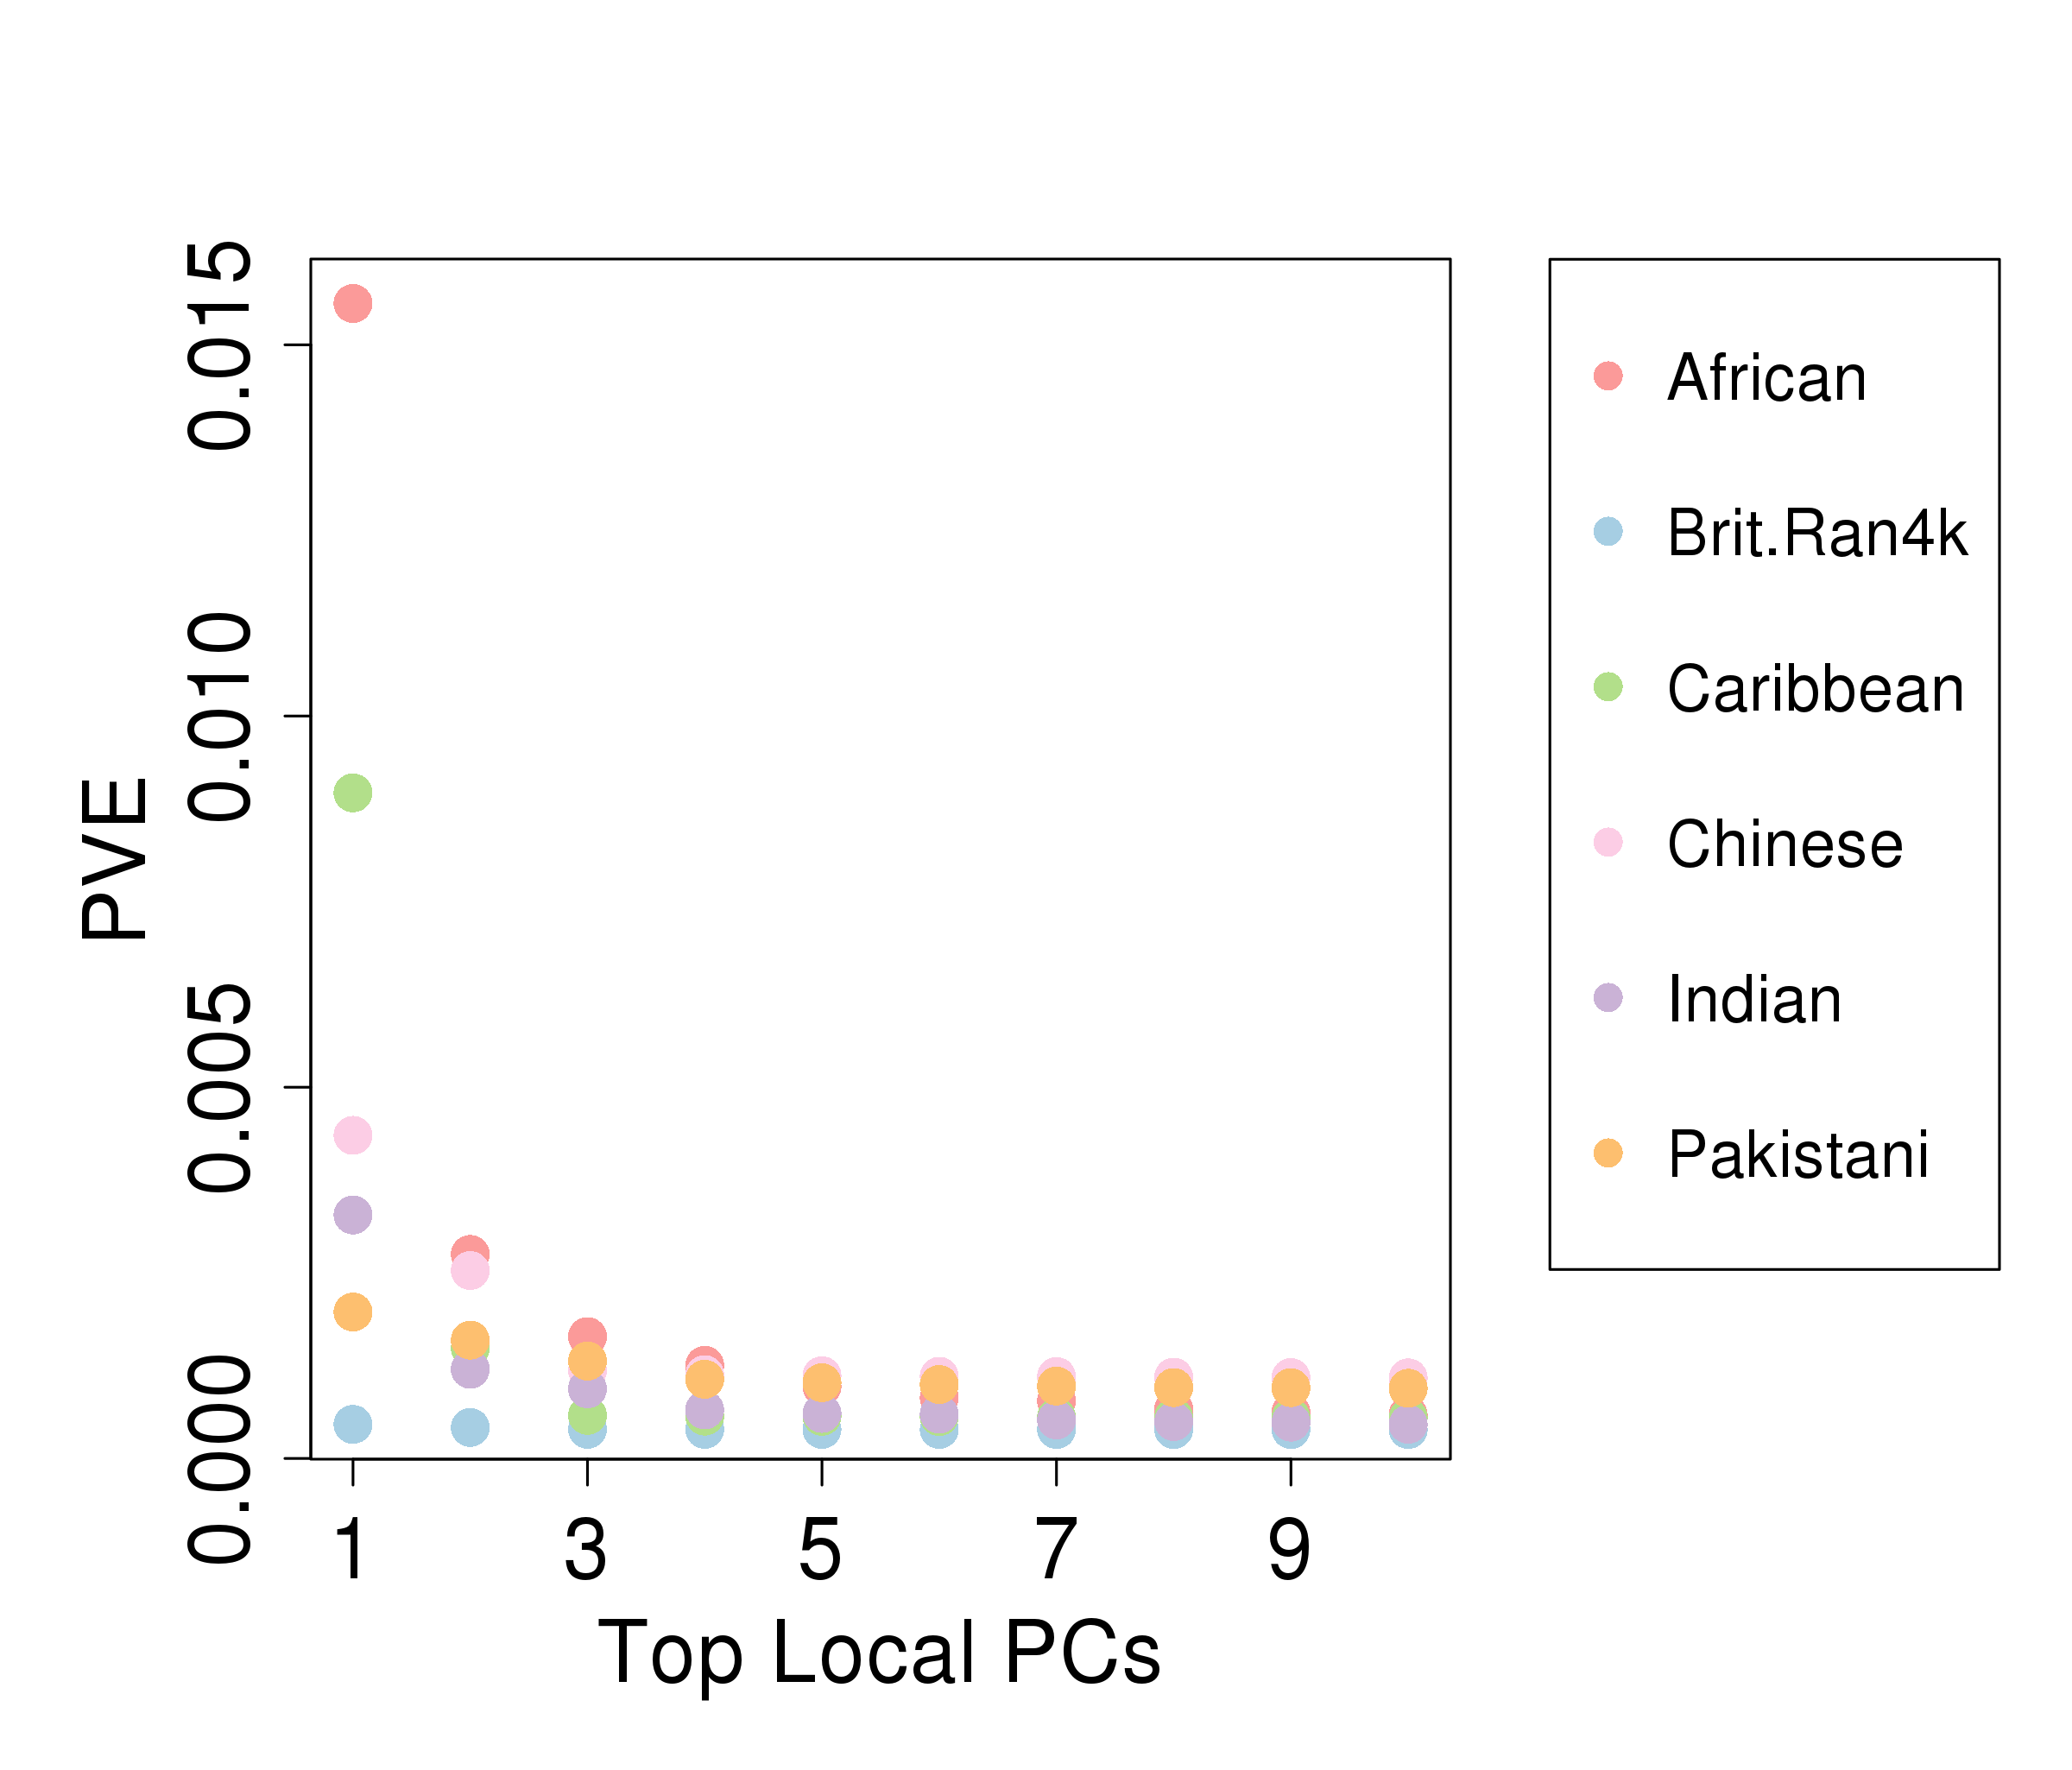
\includegraphics[scale=.45]{Images/Main/InterPath_Main_Figure_Eigenvalues_vs2.png}
\caption[TBD]{\textbf{Distribution of top 10 local principal component PVEs across UKB subgroups}. The plot shows the PVE of each of the top 10 local PCs for each of our UKB population subgroups. Local here continues to refer to calculating PCs within each subgroup separately (versus calculating PCs jointly across all subgroups together). We observe that the distribution of PC1 PVEs among the subgroups appears to match the distribution of total number of genome-wide significant MAPIT-R pathways we identify per subgroup (see Figure \ref{InterPath-Main-Figure-Barplots-KEGG} and  Supplementary Figure \ref{InterPath-Supp-Figure-Barplots-REACTOME}).}
\label{InterPath-Main-Figure-Eigenvalues}
\end{figure}

One other possibility is that PC space, while revealing a possible connection between how population structure heterogeneity among subgroups may affect MAPIT-R results, is not sensitive enough for a pathway-level analysis. Another representation of population structure that may be more ancestry-specific, and therefore more sensitive, is local ancestry estimates. Because the African subgroup contains admixture, we can test whether pathways that have a greater proportion of local African ancestry are more likely to have lower MAPIT-R $p$-values. To do this, we ran RFMix \citep{Maples2013} on the African subgroup with the 1000 Genomes CEU and YRI \citep{Genomes2015} populations as outgroups to calculate per individual estimates of local African ancestry, and we then derived subgroup-wide average local ancestry estimates across all individuals. To get final pathway-level metrics of local ancestry, we calculated the average overlap a pathway has with regions of the genome that have local African ancestry. We then tested each pathway's proportion of local African ancestry against its MAPIT-R $p$-value to see if this more ancestry-specific form of population structure has a relationship to the large number of MAPIT-R results the African subgroup has. However, as Figure \ref{InterPath-Main-Figure-RFMix-African-REACTOME} and Supplementary Figure \ref{InterPath-Supp-Figure-RFMix-African-KEGG} show, we find no relationship between a pathway's proportion of local African ancestry and its MAPIT-R $p$-value.




\begin{figure}[htb]
\centering
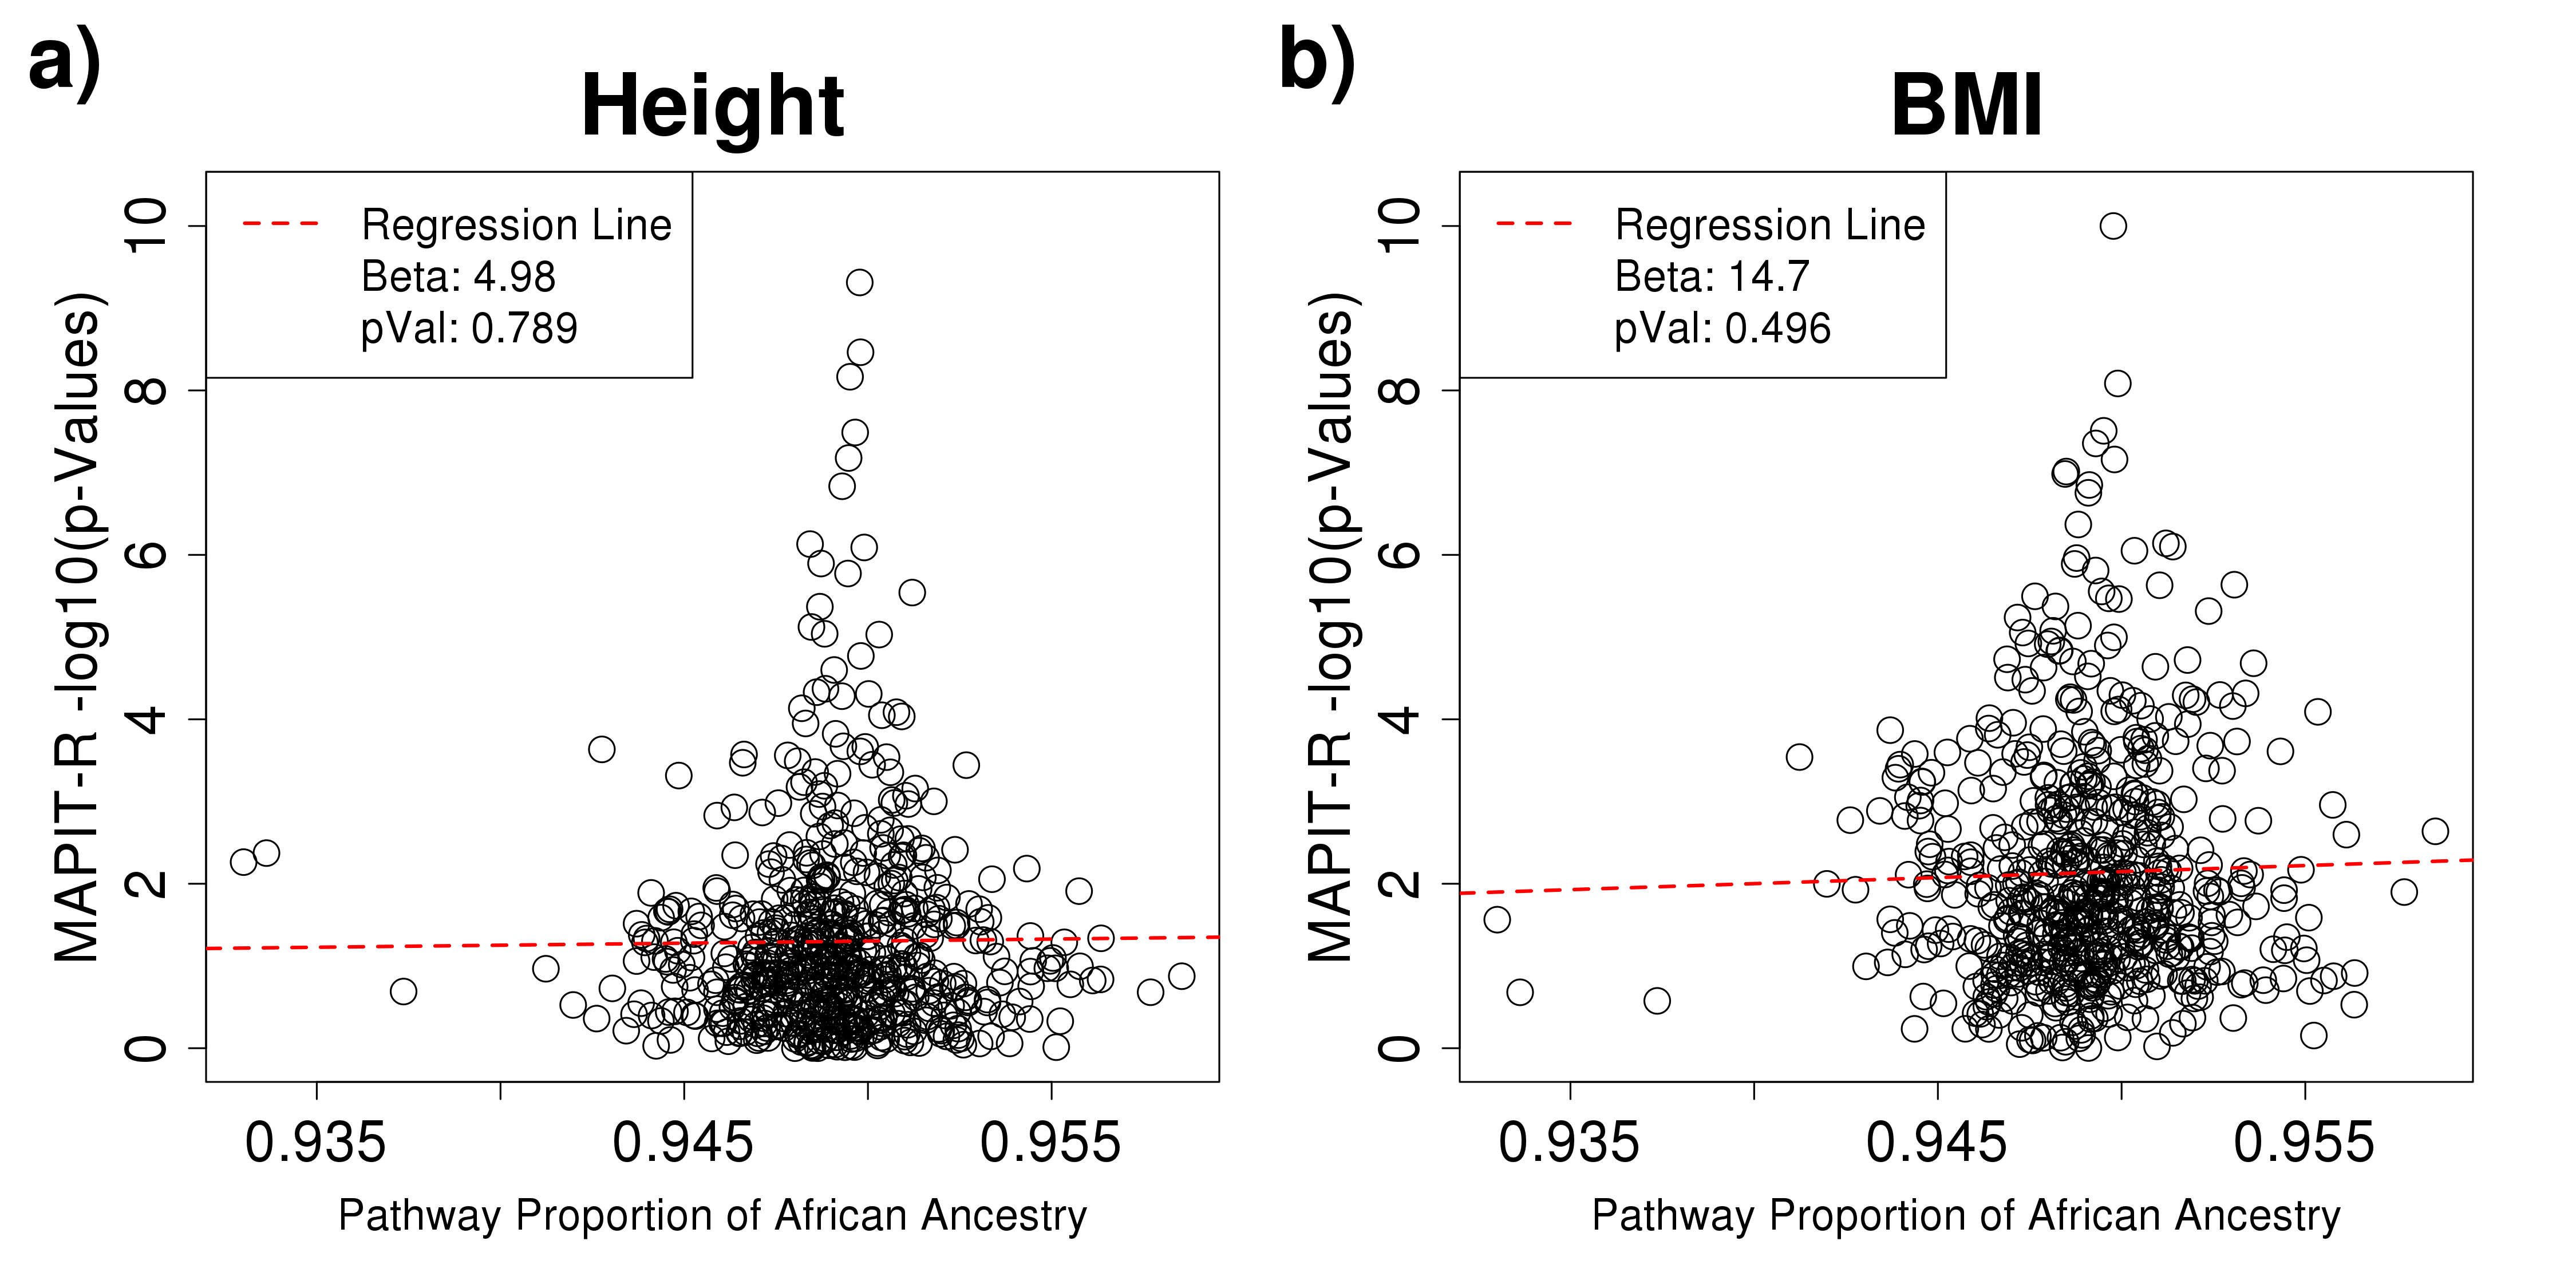
\includegraphics[scale=.35]{Images/Main/InterPath_Main_Figure_RFMix_vs2_African_REACTOME_noHLA.png}
\caption[TBD]{\textbf{MAPIT-R results vs. proportion of local African ancestry per REACTOME pathway}. The figure shows MAPIT-R $p$-values per pathway plotted against each pathway's proportion of local African ancestry for each REACTOME (a) height and (b) BMI analysis. Proportions of African ancestry are shown on the $x$-axis and MAPIT-R $p$-values are shown on the $y$-axis. African ancestry proportions were calculated per individual by using RFMix with the 1000 Genomes CEU and YRI populations as outgroups and then genome-wide averages were taken across the subgroup. Per pathway proportions of African ancestry were derived by taking the average of the subgroup-wide estimates of African ancestry across the regions of the genome that each pathway overlapped.}
\label{InterPath-Main-Figure-RFMix-African-REACTOME}
\end{figure}


\subsection*{MAPIT-R results versus genetic variation analyses}
\subsubsection*{Pathway-level IBS analyses}

Pathway-level IBS analyses were conducted by first calculating per-pathway IBS metrics. These were derived by using PLINK's \texttt{--distance ibs} function \citep{Purcell2007} using only the SNPs present in each pathway and only the individuals within each subgroup one at a time. For a single subgroup-wide metric per-pathway, the average pathway IBS value was taken across all pairwise comparisons within a given subgroup. Comparisons were then made by comparing this single subgroup-wide, per-pathway IBS metric against each pathway's original MAPIT-R $p$-value.

\subsubsection{RFMix analyses}

RFMix analyses were conducted within the African subgroup by running local ancestry estimation with RFMix v2.03 \citep{Maples2013} and the 1000 Genomes CEU and YRI populations \citep{Genomes2015} as outgroups. Pathway-level metrics of local ancestry were then calculated by first taking the average local African estimates across all individuals within the subgroup for a given genomic region and then averaging these subgroup-wide values across all portions of the genome a pathway overlaps. This produced a single per-pathway metric of local African ancestry that was then used to compare against MAPIT-R $p$-values. Running two iterations of the RFMix EM step to refine local ancestry estimates did not change the results.

\subsubsection{PC1 SNP loading analyses}

PC1 SNP loading analyses were conducted by first calculating per-pathway metrics of PC1 SNP loading proportions. This was done by: a) deriving PC1 loading scores per SNP by projecting all SNPs back onto the `local' PC space previously calculated within each subgroup, b) determining the distribution of local PC1 loading scores across all SNPs and designating SNPs within the 2.5\% tails of these distributions as `strongly loaded' on PC1, and c) calculating the proportion of SNPs per pathway that are designated as local PC1 `strongly loaded'. Given these per-pathway proportions of `strongly loaded' local PC1 SNPs then, comparisons where made between them and each pathway's MAPIT-R $p$-value. Using percent thresholds of 5\% or 10\% in the tails of the local PC1 loading score distributions to determine `strongly loaded' SNPs did not change the results (data not shown).




%%%%%%%%%%
%%%%%%%%%%



\section{Supplementary Note}\label{Supplementary-Note}

\subsection{Population Subgroup Quality Control}

We conducted standard quality control (QC) procedures on each of these population subgroups. Note that we focused our analyzes on the genotyped chip data throughout the project. First we conducted SNP-level QC by dropping variants that did not meet the following criteria:  minor allele frequency (MAF) $>$ .01, genotype missingness $<$ 5\%, and Hardy-Weinberg equilibrium test $p$-value $>$ $1\times10^{-6}$. We then conducted individual-level QC via the following steps. Individuals were removed if they did not have genotype missingness $>$ 5\%. Individuals were also removed if they were a 3\textsuperscript{rd} degree relative or more to someone else in the dataset; specifically the KING relatedness values provided with the UKB data were used to identify related individuals, and one individual from every pair of 3\textsuperscript{rd} degree or more relatives was removed. Individuals were also dropped if they were tagged by any of the following three flags from the UKB data: `het.missing.outliers', `putative.sex.chromosome.aneuploidy', and `excess.relatives'. Lastly, individuals were removed if they were determined to be PCA outliers; this was conducted by running FlashPCA (version 2.1) \citep{Abraham2017} in R on each population subgroup separately and identifying individuals that had PC values greater than 7 standard deviations away from the mean for any of the top 6 PCs. We refer to conducting PCA on each subgroup separately as 'local PCA' to help distinguish from the alternative setup of conducting PCA on the entire dataset jointly, which would be referred to as 'global PCA'. 

After this first round of QC procedures, we then proceeded to impute our current population subgroups. Since most of the analyses in this project utilized genetic relatedness matrices (GRMs), and variants need to have no missing data for these GRMs, we used imputation primarily to maximize the number of genotyped SNPs that would not be dropped by this stringent threshold (as opposed to using imputation to increase the number of SNPs we were analyzing). To conduct this imputation, we uploaded our population subgroups to the University of Michigan Imputation Server \citep{Das2016} and used the following options: Minimac3 for the imputation software, 1000G phase 3 v5 for the reference panel, and Eagle v2.3 for the phasing software. Completed imputed files were then downloaded from the Imputation Server afterwards and treated to further QC steps: imputed variants were intersected back to the original set of genotyped chip variants, variants with imputation quality scores $<$ .3 were removed, and variants that had genotype missingness rates $>$ 0\% were also removed. These steps represent the last of our QC and imputation procedures, and information on the final forms of our UKB population subgroups can be found in Supplementary Table (table).

\clearpage

\section{Supplementary Figures}\label{Supplementary-Figures}

%\renewcommand{\thefigure}{Supplementary Figure \arabic{figure}}
%\renewcommand{\thetable}{Supplementary \arabic{table}}
\renewcommand{\figurename}{Supplementary Figure}
\renewcommand{\tablename}{Supplementary Table}
\setcounter{figure}{0}
\setcounter{table}{0}

\begin{figure}[htbp]
\centering
\hspace*{-1cm}
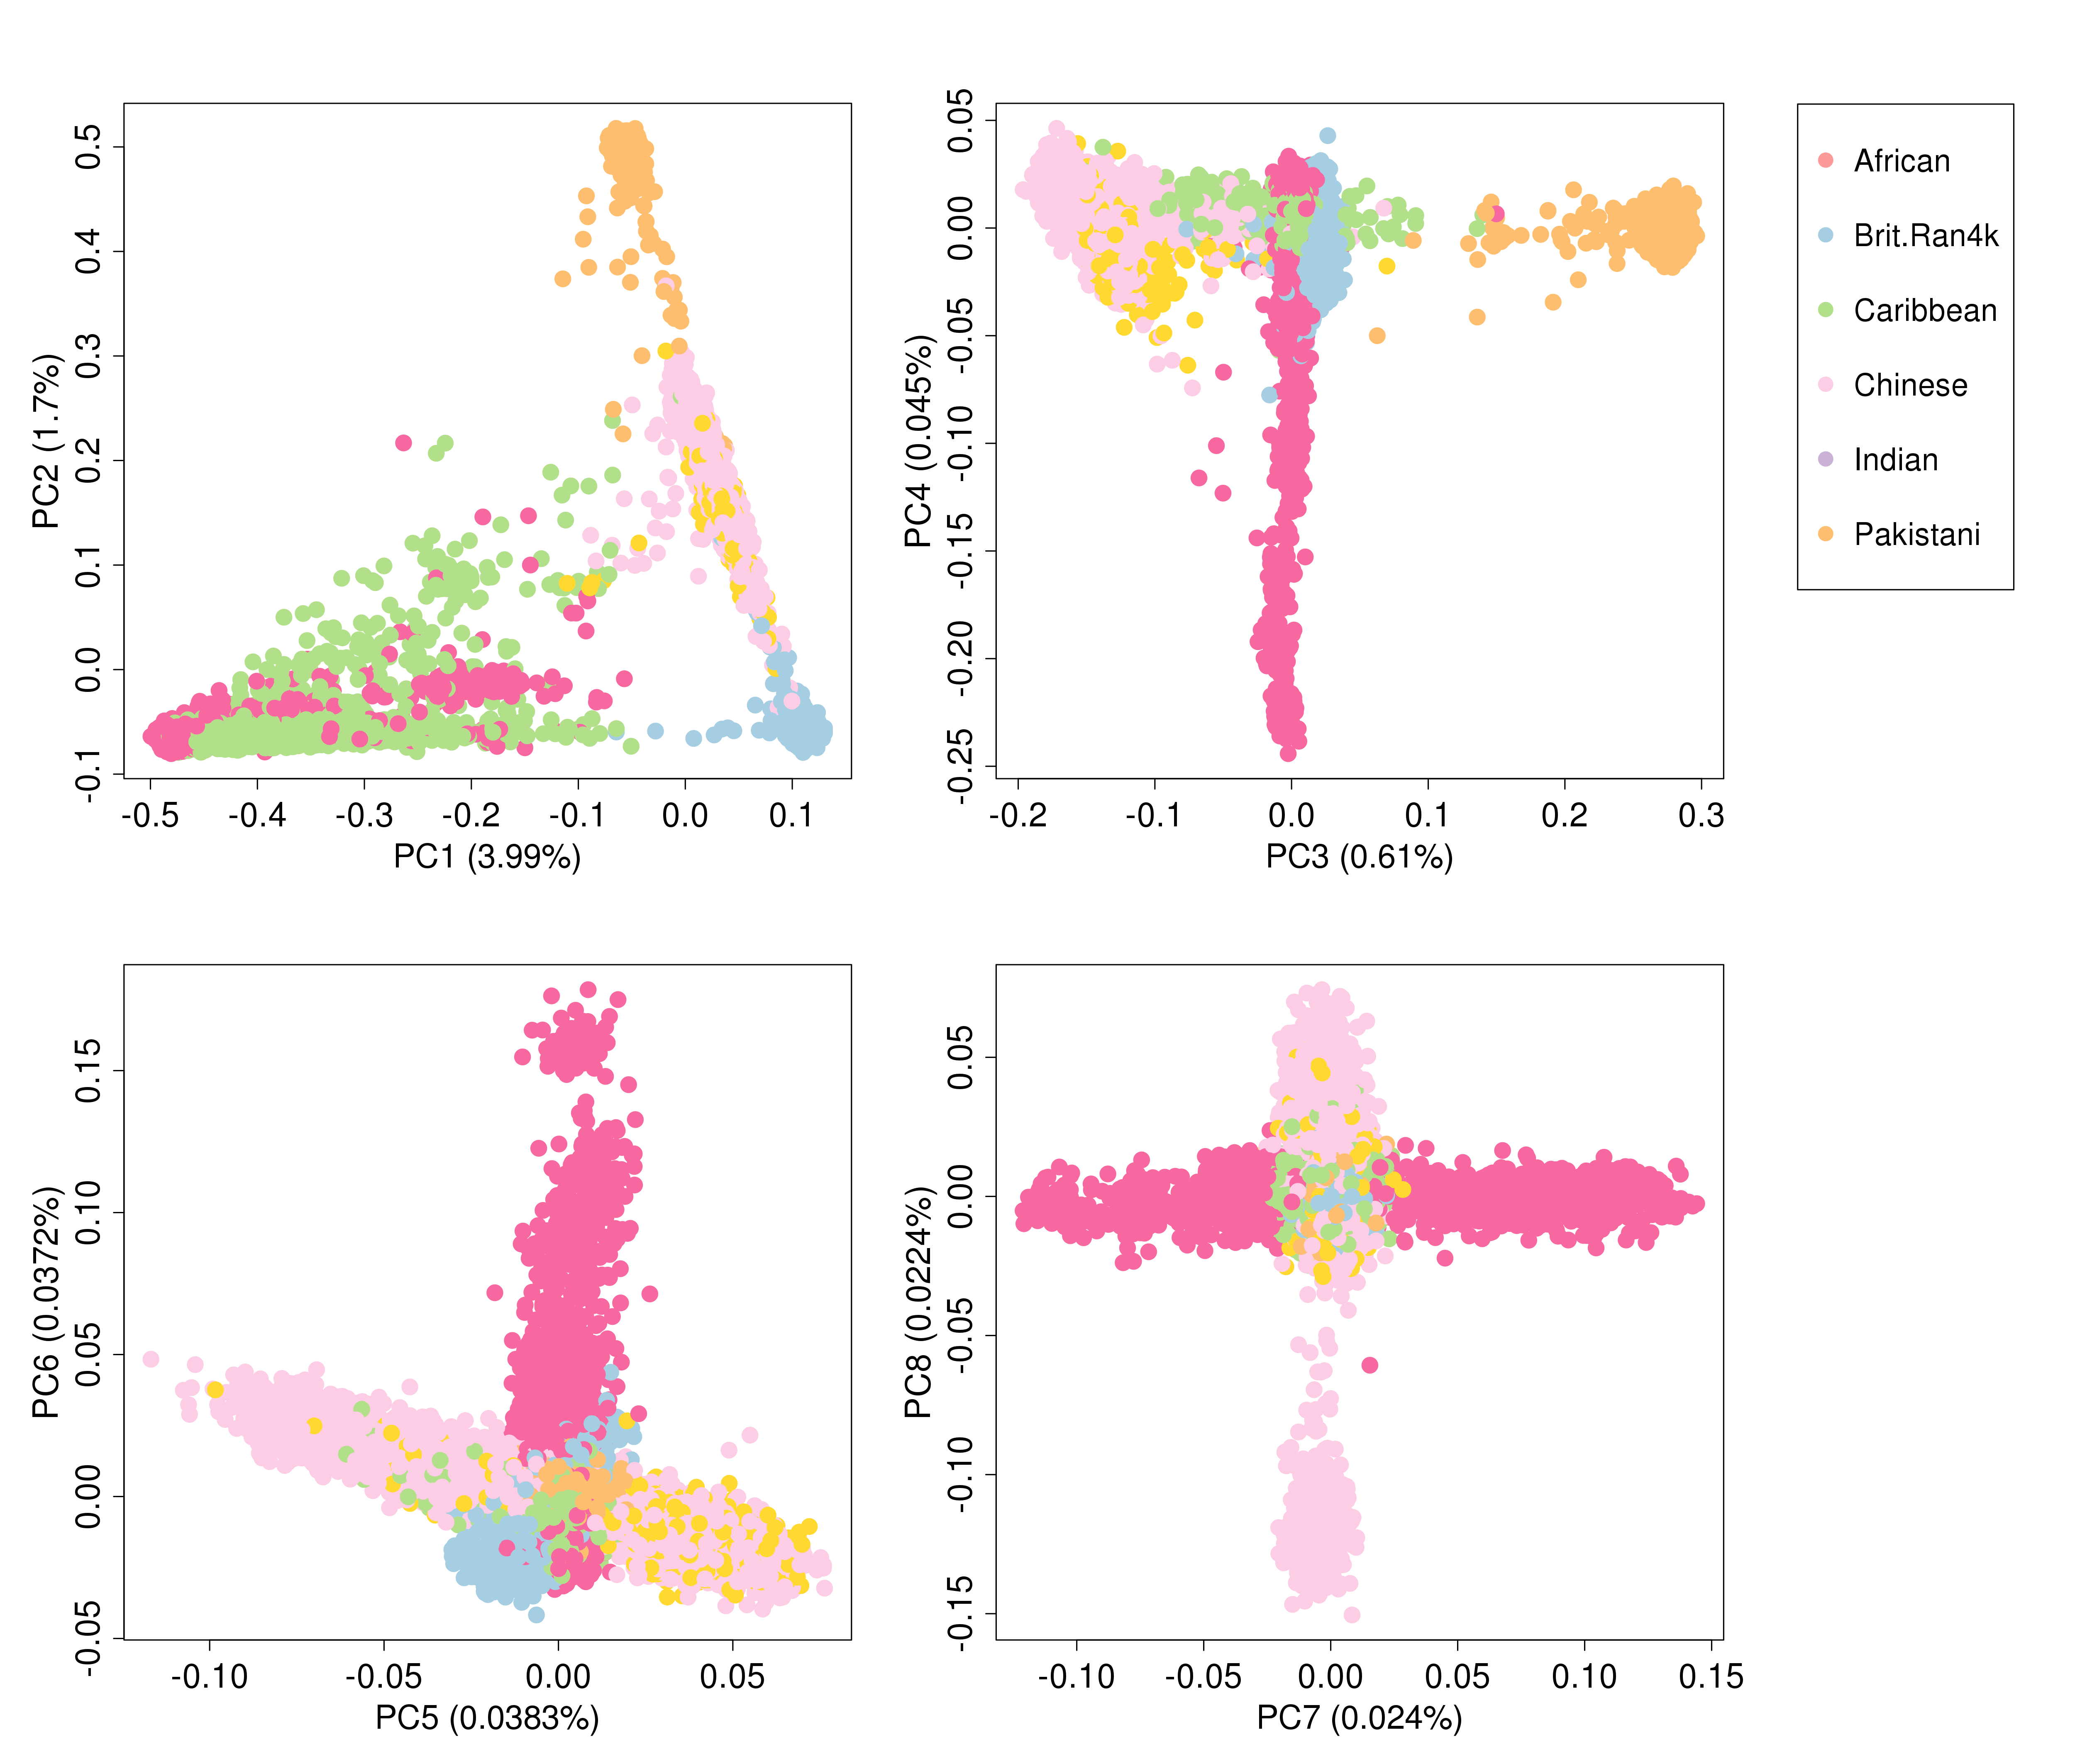
\includegraphics[scale=.4]{Images/Supp/InterPath_Supp_Figure_UKB_PCAPlot_vs2.png}
\caption[TBD]{\textbf{Global PCA Plots of the UK BioBank subgroups}. The figure shows the top eight global principal components (PCs) of our UKB subgroup dataset plotted against one another: (a) PC1 vs. PC2, (b) PC3 vs. PC4, (c) PC5 vs. PC6, and (d) PC7 vs. PC8. PCA was conducted using FlashPCA \citep{Abraham2017} and a post-QC, pruned SNP set. Here `Global' PCs refers to PCs calculated from running PCA on the full dataset of all subgroups together jointly. This is in contrast to `local' PCs, which are calculated by running PCA on each subgroup separately. As a result of this difference, global PCs were created similar to the descriptions in `Population subgroups' of Methods and `Population Subgroup Quality Control' of Supplementary Note, but in lieu of running FlashPCA on each subgroup separately, FlashPCA was run on the full dataset together jointly. Global PCs were only used for these plots, and local PCs were used for quality control and as covariates. In parentheses next to each PC is the percent variance explained (PVE) each PC accounts for of the total variation present in the underlying covariance matrix.}
\label{InterPath-Supp-Figure-UKB-subgroups-PCAPlot}
\end{figure}
\clearpage

\begin{figure}[htbp]
\centering
\hspace*{-.9cm}
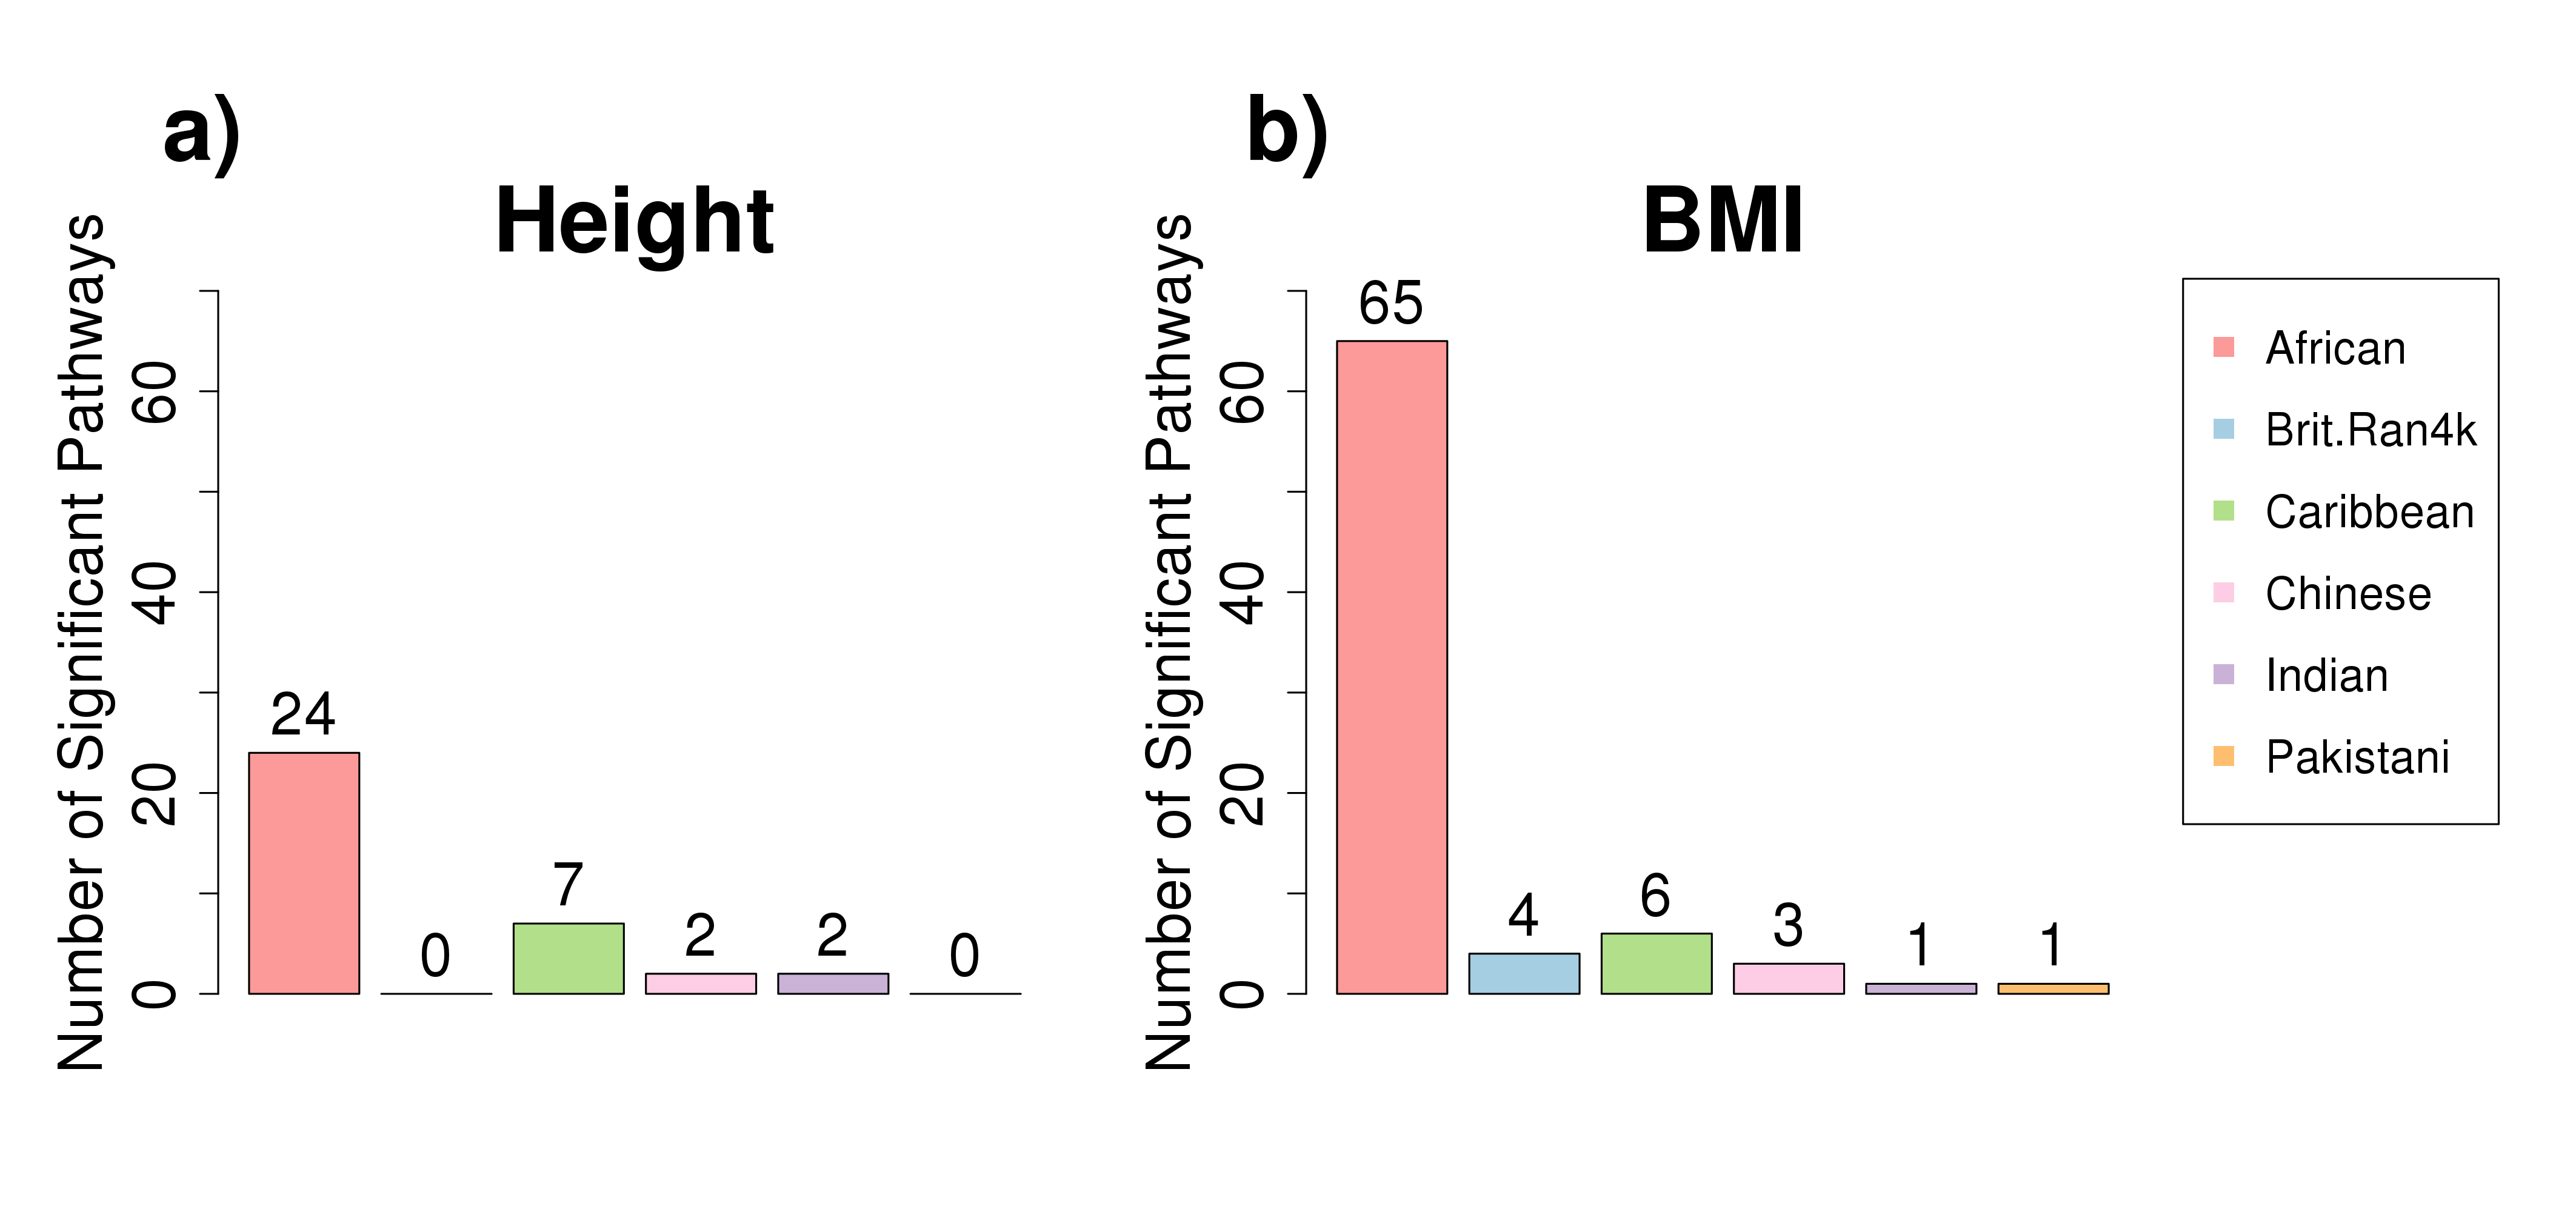
\includegraphics[scale=.45]{Images/Supp/InterPath_Supp_Figure_Barplots_REACTOME_vs4.png}
\caption[TBD]{\textbf{Numbers of REACTOME pathways that have significant marginal epistasis, per subgroup}. The barplots show the number of genome-wide significant pathways found from running MAPIT-R for both (a) height and (b) BMI in the REACTOME database on each of our UKB subgroups. Genome-wide significance was determined by using Bonferroni-corrected $p$-value thresholds based on the number of pathways tested in each pathway database-phenotype-subgroup combination. As shown in these results, we find across all database-phenotype combinations that the African subgroup has the largest numbers of significant pathways. For lists of the specific significant pathways per database-phenotype-subgroup combination, see Supplementary Tables \ref{InterPath-Supp-Table-TopPathways-AllPaths-AllPhenos}\textcolor{blue}{a-d}.}
\label{InterPath-Supp-Figure-Barplots-REACTOME}
\end{figure}
\clearpage

\begin{figure}[htbp]
\centering
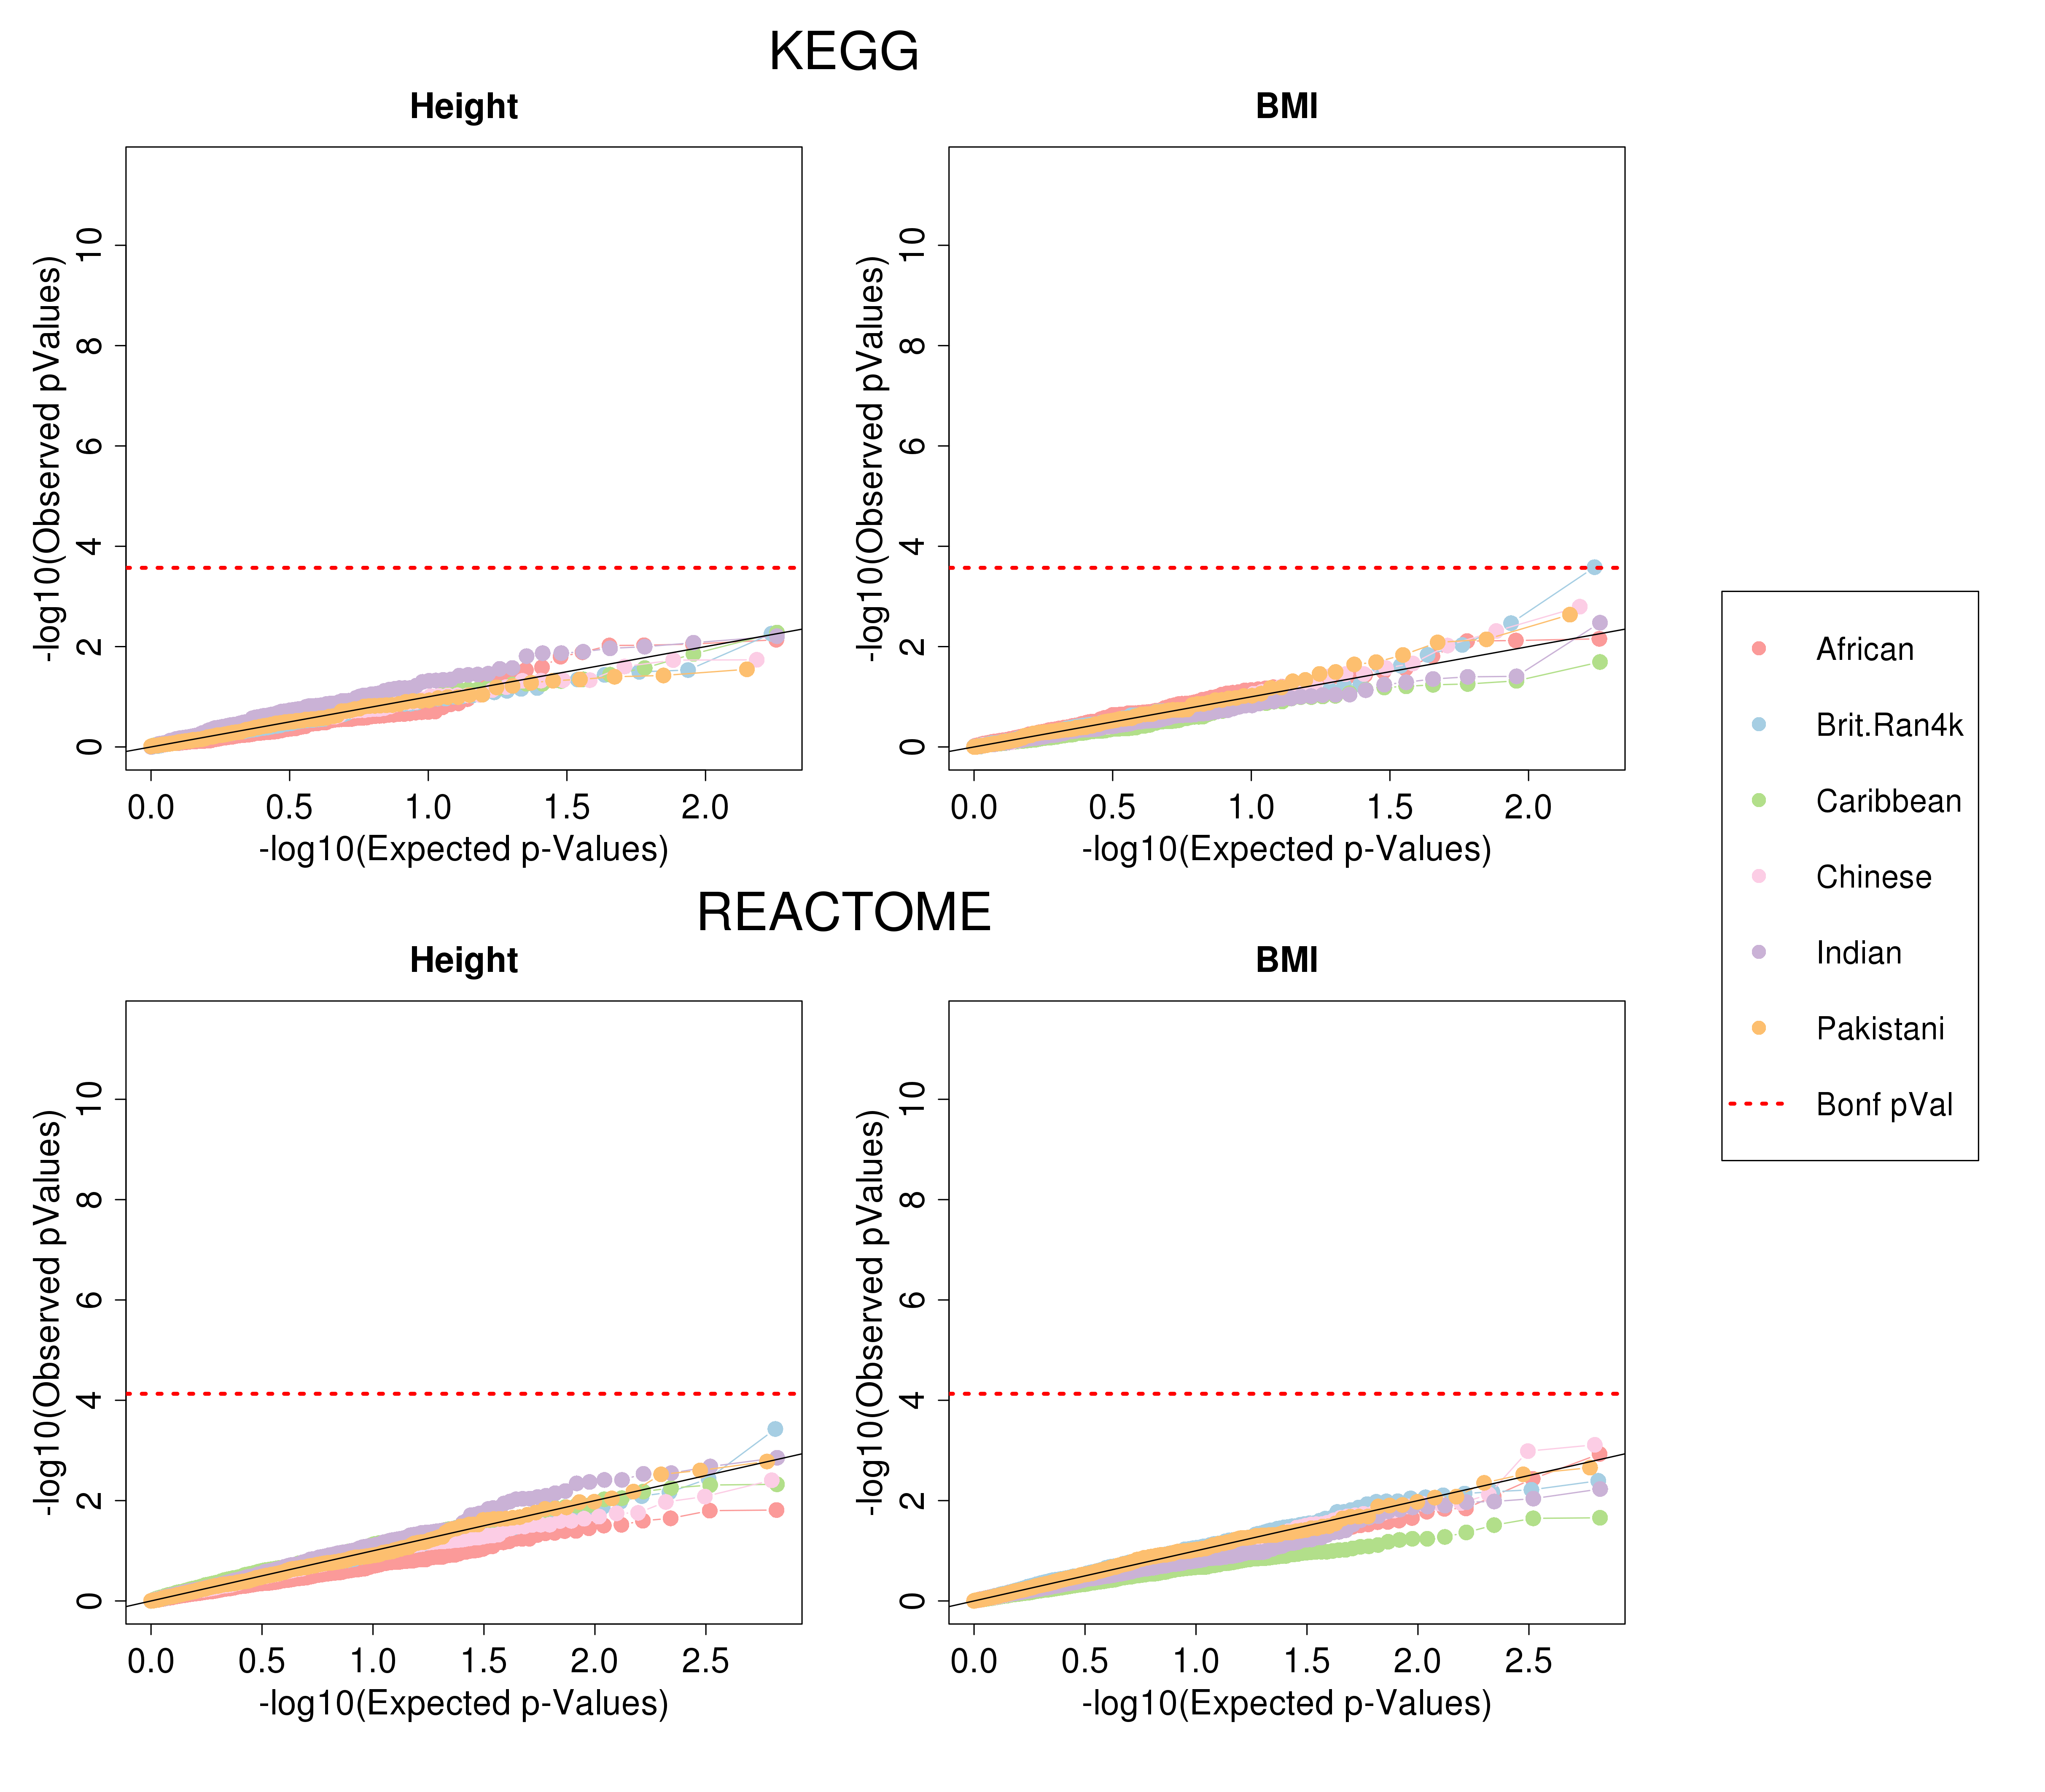
\includegraphics[scale=.35]{Images/Supp/InterPath_Supp_Figure_perm1_QQPlots_AllPaths_vs2.png}
\caption[TBD]{\textbf{QQ-Plots of MAPIT-R results using permuted phenotypes, per subgroup}. The figure shows QQ-plots for running MAPIT-R using a single permutation of either height or BMI measurements within the KEGG and REACTOME databases. Phenotypes were permuted within each population subgroup. Shown on the $x$-axis are the -$\log_{10}$ of the expected $p$-values and the on the $y$-axis are on the -$\log_{10}$ of the observed $p$-values. The dotted red line is the Bonferroni-corrected $p$-value threshold based on the number of pathways tested per pathway database-phenotype combination (Supplementary Table \ref{InterPath-Supp-Table-UKBPopStats}). Looking in total across the ten permutation runs conducted for each pathway database-phenotype-UKB subgroup combination, we find that MAPIT-R properly controls for the false positive rate at varying significance cutoff thresholds (Supplementary Figure \ref{InterPath-Supp-Table-BritReps-FDRs-pt1}).}
\label{InterPath-Supp-Figure-perm1-QQPlots-AllPaths}
\end{figure}
\clearpage

\setlength{\footskip}{3cm}
\begin{figure}[htbp]
\centering
\vspace*{-2cm}
\includegraphics[scale=.2]{Images/Supp/InterPath_Supp_Figure_pValHists_vs3.png}
\caption[TBD]{\textbf{$p$-Value histograms of MAPIT-R results using permuted phenotypes, per subgroup}. The figure shows histograms of MAPIT-R $p$-values collected across ten independent phenotype permutation runs for each UKB subgroup (Supplementary Table \ref{InterPath-Supp-Table-UKBPopStats}). The same phenotype permutation for a given subgroup was used across both pathway databases (i.e. 10 permutations were done for height and 10 done for BMI for each subgroup). And the same covariates used per individual from the original MAPIT-R analysis were used for these permuted-phenotype analyses (see Materials and Methods).}
\label{InterPath-Supp-Figure-10perms-pValHists}
\end{figure}
\clearpage
\setlength{\footskip}{1cm}

\setlength{\footskip}{1cm}
\begin{figure}[htbp]
\centering
\vspace*{-2cm}
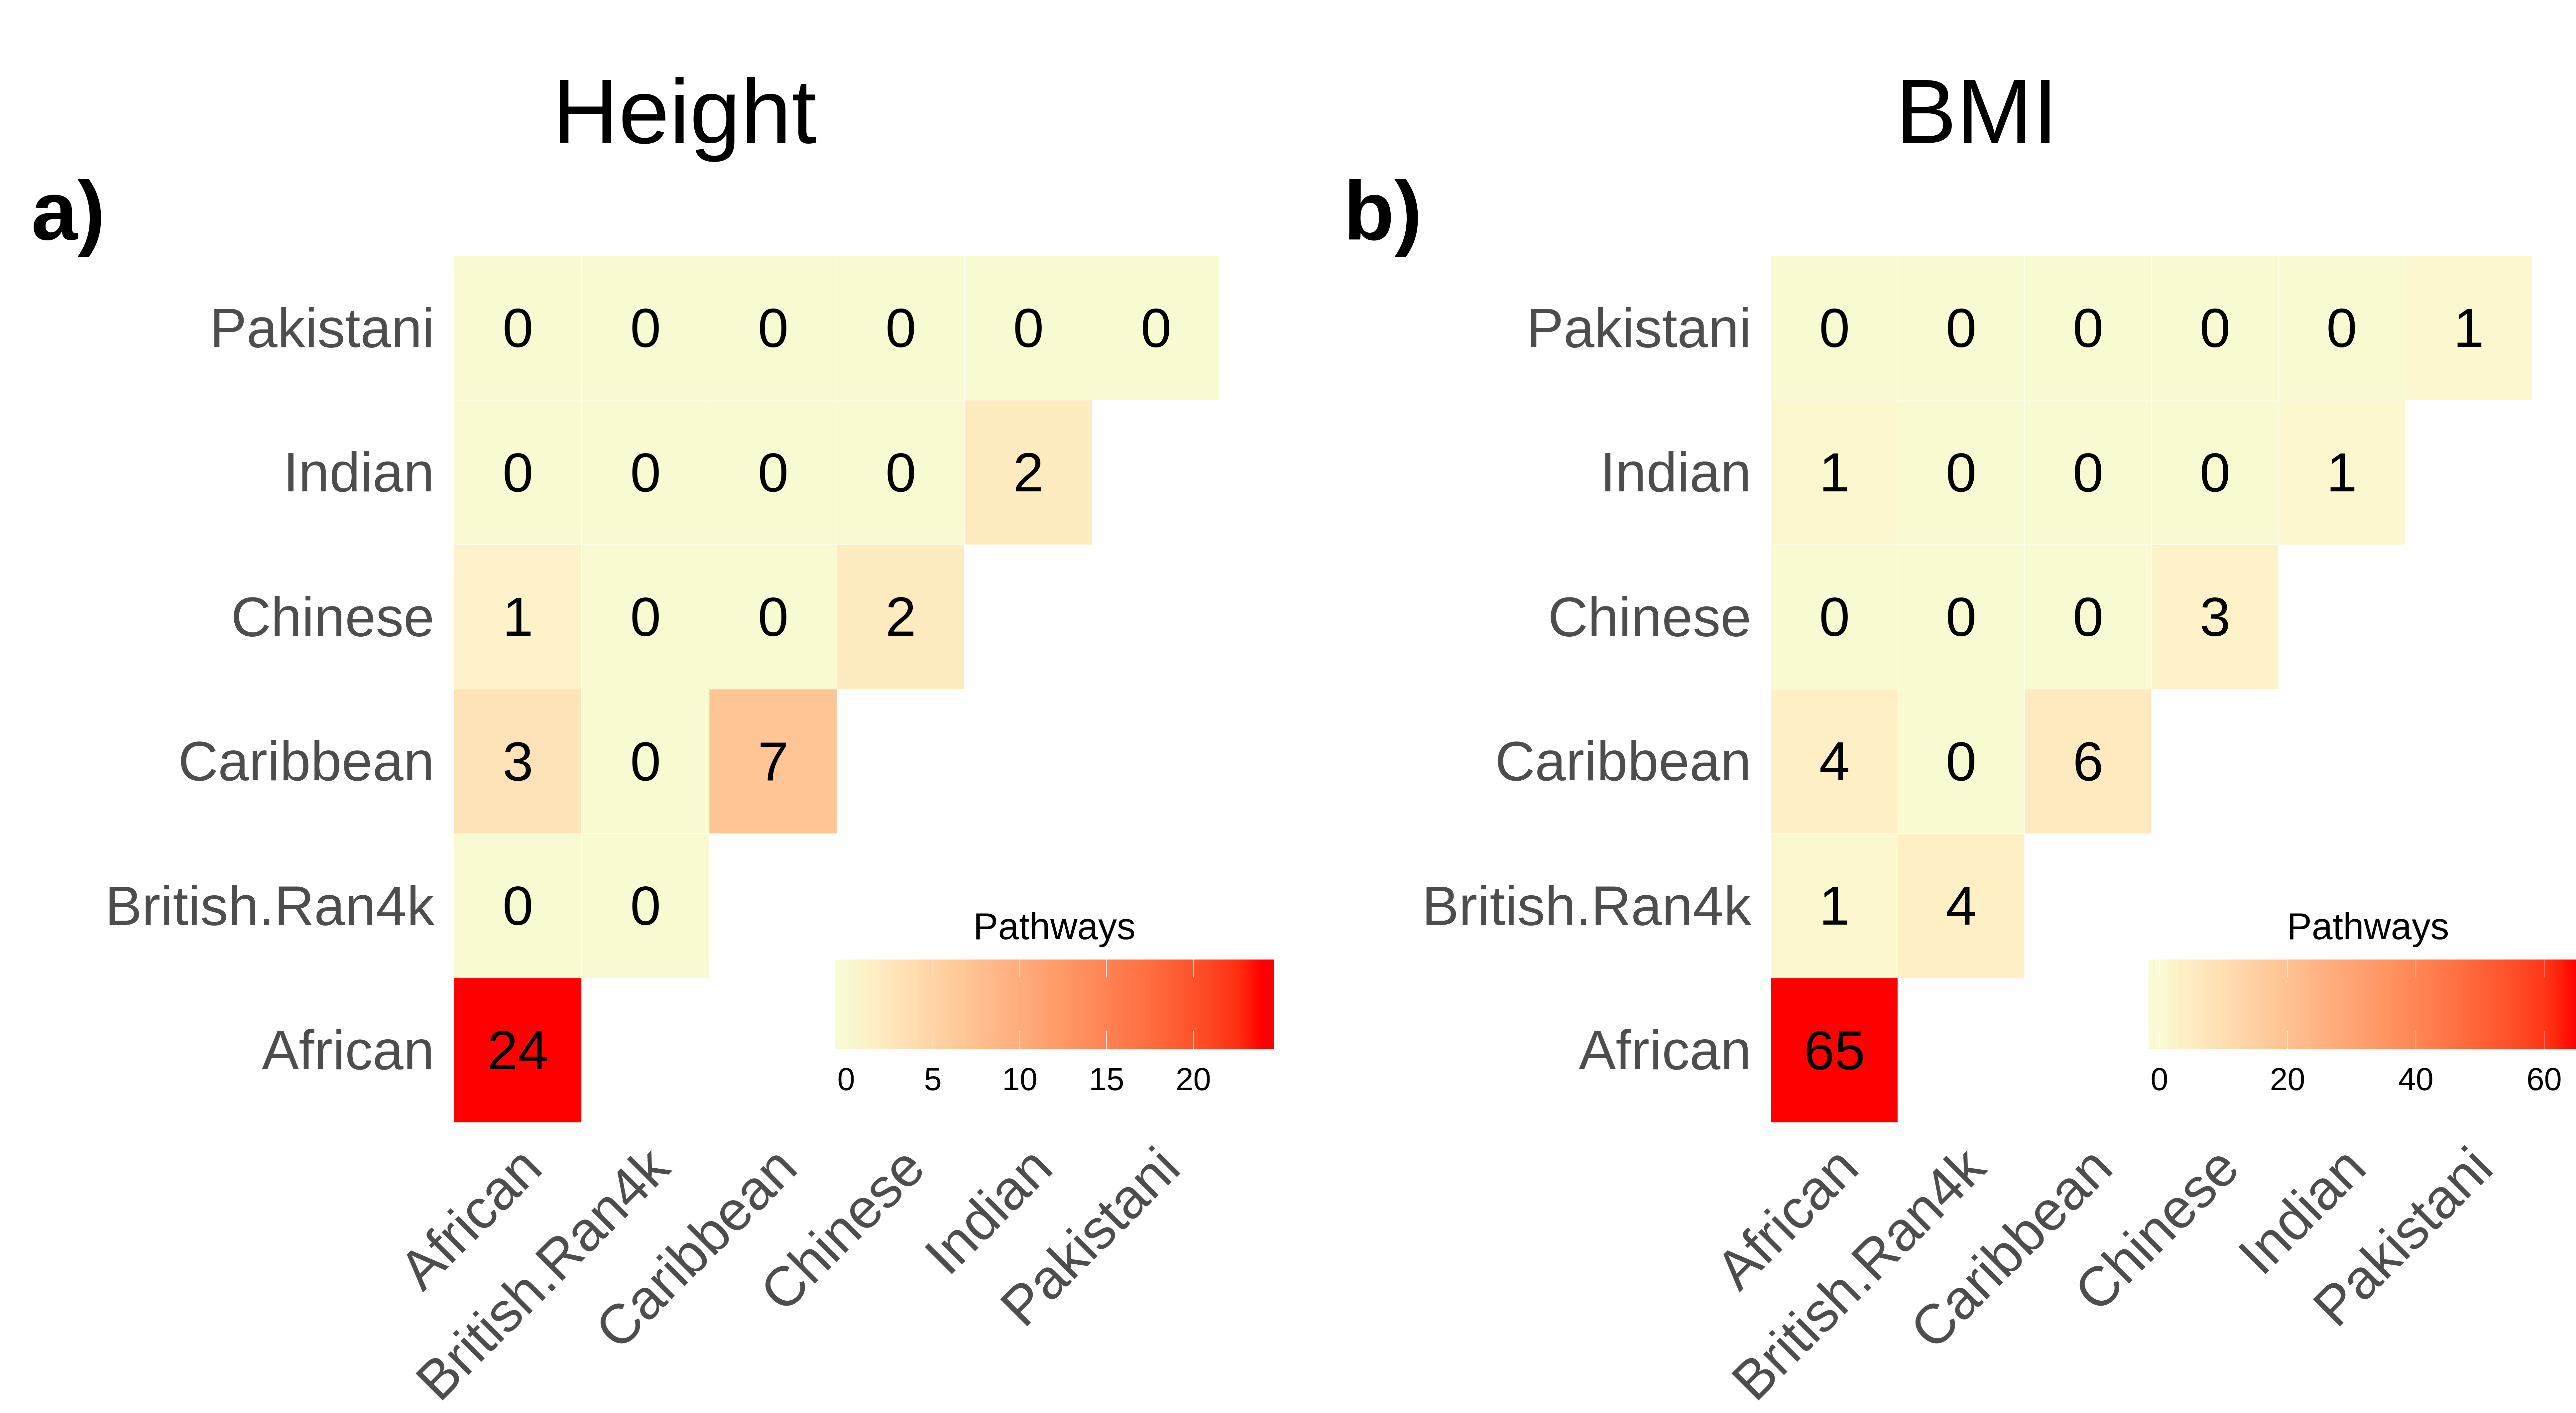
\includegraphics[scale=.225]{Images/Supp/InterPath_Supp_Figure_Heatplots_REACTOME_vs4.png}
\caption[TBD]{\textbf{Overlap of genome-wide significant MAPIT-R pathways between UKB population subgroups: REACTOME}. The heatplots show the numbers of genome-wide significant MAPIT-R pathways that overlap between each UKB subgroup for (a) height and (b) BMI in the REACTOME database. The diagonal shows the total number of genome-wide significant pathways per population subgroup. We observe that most subgroups often have overlap with the African subgroup but rarely do so with the remaining non-African subgroups. For results from the KEGG database see Figure \ref{InterPath-Main-Figure-Heatplots-KEGG}.}
\label{InterPath-Supp-Figure-Heatplots-REACTOME}
\end{figure}
\clearpage
\setlength{\footskip}{1cm}

\setlength{\footskip}{3cm}
\begin{figure}[htbp]
\centering
\vspace*{-2cm}
\includegraphics[scale=.2]{Images/Supp/InterPath_Supp_Figure_MAPITR_PhenoComps_AllPops_vs4.png}
\caption[TBD]{\textbf{Comparison of MAPIT-R results between height and BMI, per subgroup}. The figure shows MAPIT-R height results plotted against MAPIT-R BMI results for all pathways from the KEGG and REACTOME databases in all UKB subgroups. The $x$-axes are the MAPIT-R height -$\log_{10}$ $p$-values and the $y$-axes are the MAPIT-R BMI -$\log_{10}$ $p$-values. The dotted red lines are the Bonferroni-corrected $p$-value thresholds for genome-wide significance in each pathway-phenotype-subgroup combination. The correlation between the phenotype -$\log_{10}$ $p$-values is shown in the bottom right.}
\label{InterPath-Supp-Figure-MAPITR-PhenoComps-AllPops}
\end{figure}
\clearpage
\setlength{\footskip}{1cm}

\begin{figure}[htbp]
\centering
\hspace*{-1.75cm}
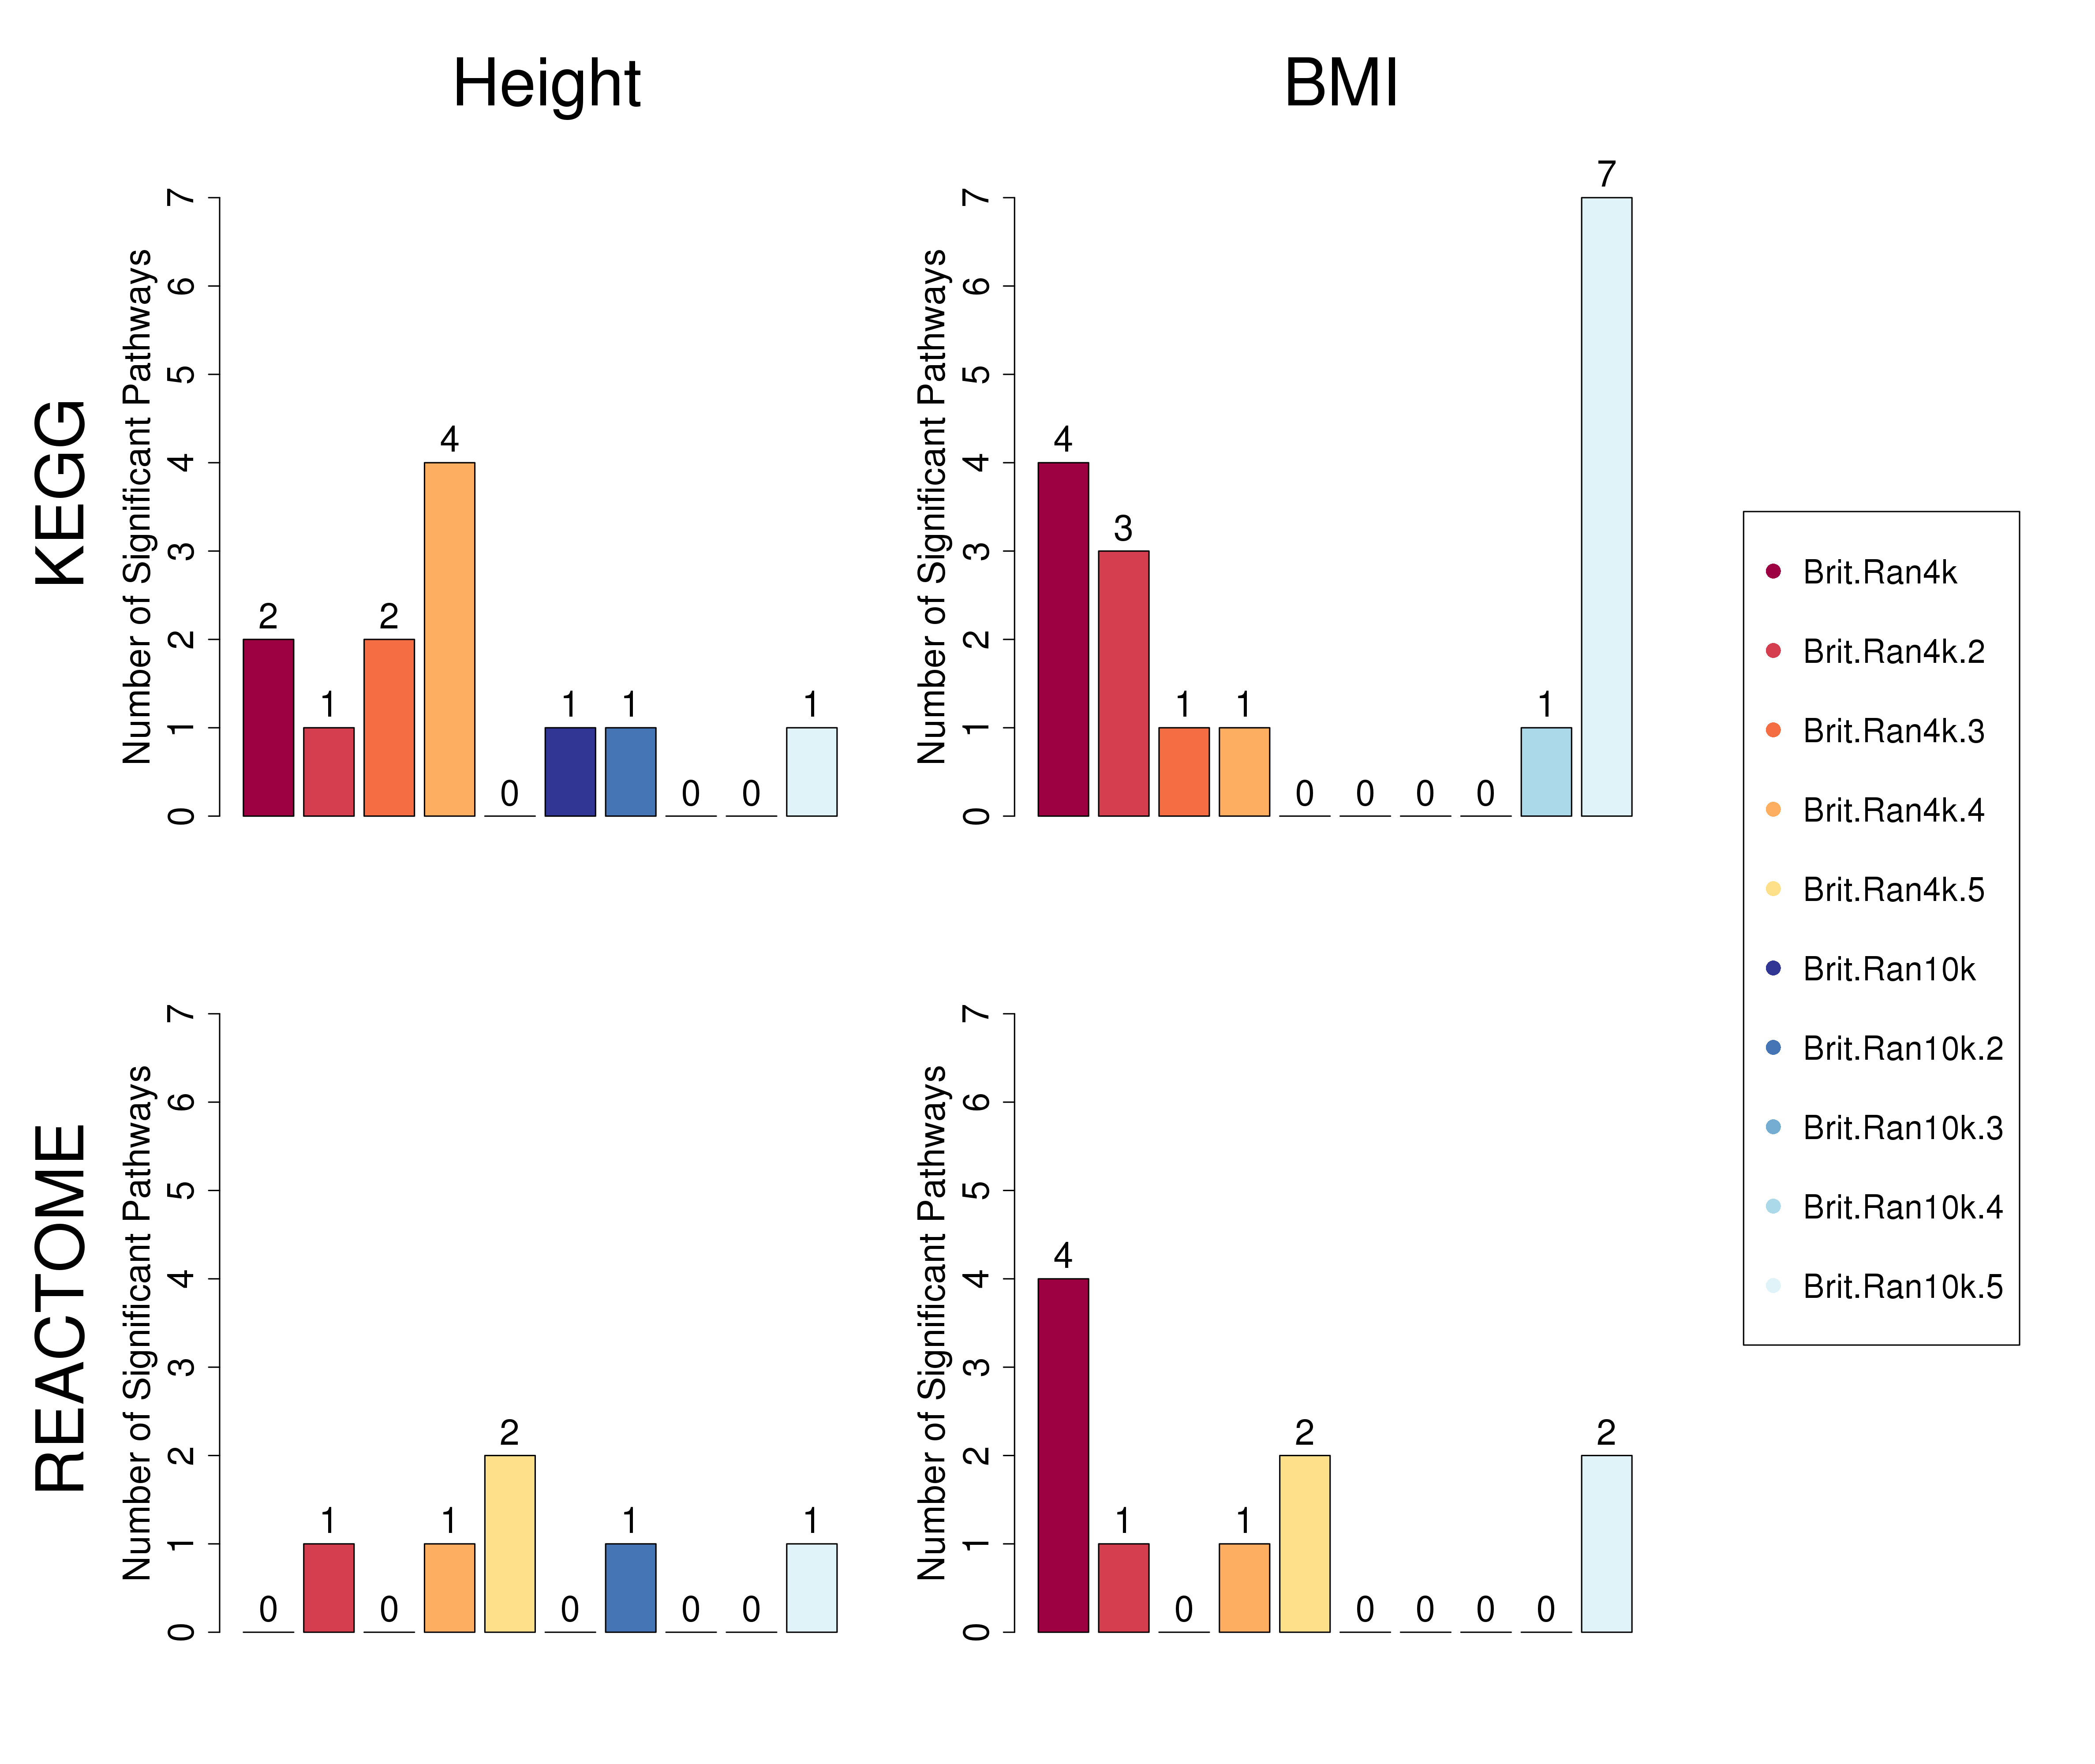
\includegraphics[scale=.45]{Images/Supp/InterPath_Supp_Figure_BritReps_Barplot_vs4.png}
\caption[TBD]{\textbf{Numbers of pathways that have significant marginal epistasis, per British replicate}. The barplots show the number of genome-wide significant pathways found from running MAPIT-R for both height and BMI in the KEGG and REACTOME databases on each of the British subsample replicate subgroups we analyzed. Genome-wide significance was determined by using Bonferroni-corrected $p$-value thresholds based on the number of pathways tested in each pathway database-phenotype-subgroup combination. Most replicate runs did not produce many significant results.}
\label{InterPath-Supp-Figure-BritReps-Barplots}
\end{figure}
\clearpage

\newcounter{CharNumber4}
\setcounter{CharNumber4}{1}
\renewcommand{\thefigure}{\arabic{figure}\alph{CharNumber4}}
\begin{landscape}
\begin{figure}[htbp]
\centering
\includegraphics[scale=.2]{Images/Supp/InterPath_Supp_Figure_BritReps_Heatplots_KEGG_vs4.png}
\caption[TBD]{\textbf{Overlap of genome-wide significant MAPIT-R pathways between British replicate subgroups: KEGG}. The heatplots show the numbers of genome-wide significant MAPIT-R pathways that overlap between each British replicate subgroup for (a) height and (b) BMI in the KEGG database. The diagonal shows the total number of genome-wide significant pathways per population subgroup. We do not observe many genome-wide significant pathways or pathways that overlap between replicate subgroups.}
\label{InterPath-Supp-Figure-BritReps-Heatplots-AllPaths-KEGG}
\end{figure}
\clearpage
\addtocounter{figure}{-1}
\addtocounter{CharNumber4}{1}
\end{landscape}

\begin{landscape}
\begin{figure}[htbp]
\centering
\includegraphics[scale=.2]{Images/Supp/InterPath_Supp_Figure_BritReps_Heatplots_REACTOME_vs4.png}
\caption[TBD]{\textbf{Overlap of genome-wide significant MAPIT-R pathways between British replicate subgroups: REACTOME}. The heatplots show the numbers of genome-wide significant MAPIT-R pathways that overlap between each British replicate subgroup for (a) height and (b) BMI in the REACTOME database. The diagonal shows the total number of genome-wide significant pathways per population subgroup. We do not observe many genome-wide significant pathways or pathways that overlap between replicate subgroups.}
\label{InterPath-Supp-Figure-BritReps-Heatplots-AllPaths-REACTOME}
\end{figure}
\clearpage
\end{landscape}
\renewcommand{\thefigure}{\arabic{figure}}

\begin{figure}[htbp]
\centering
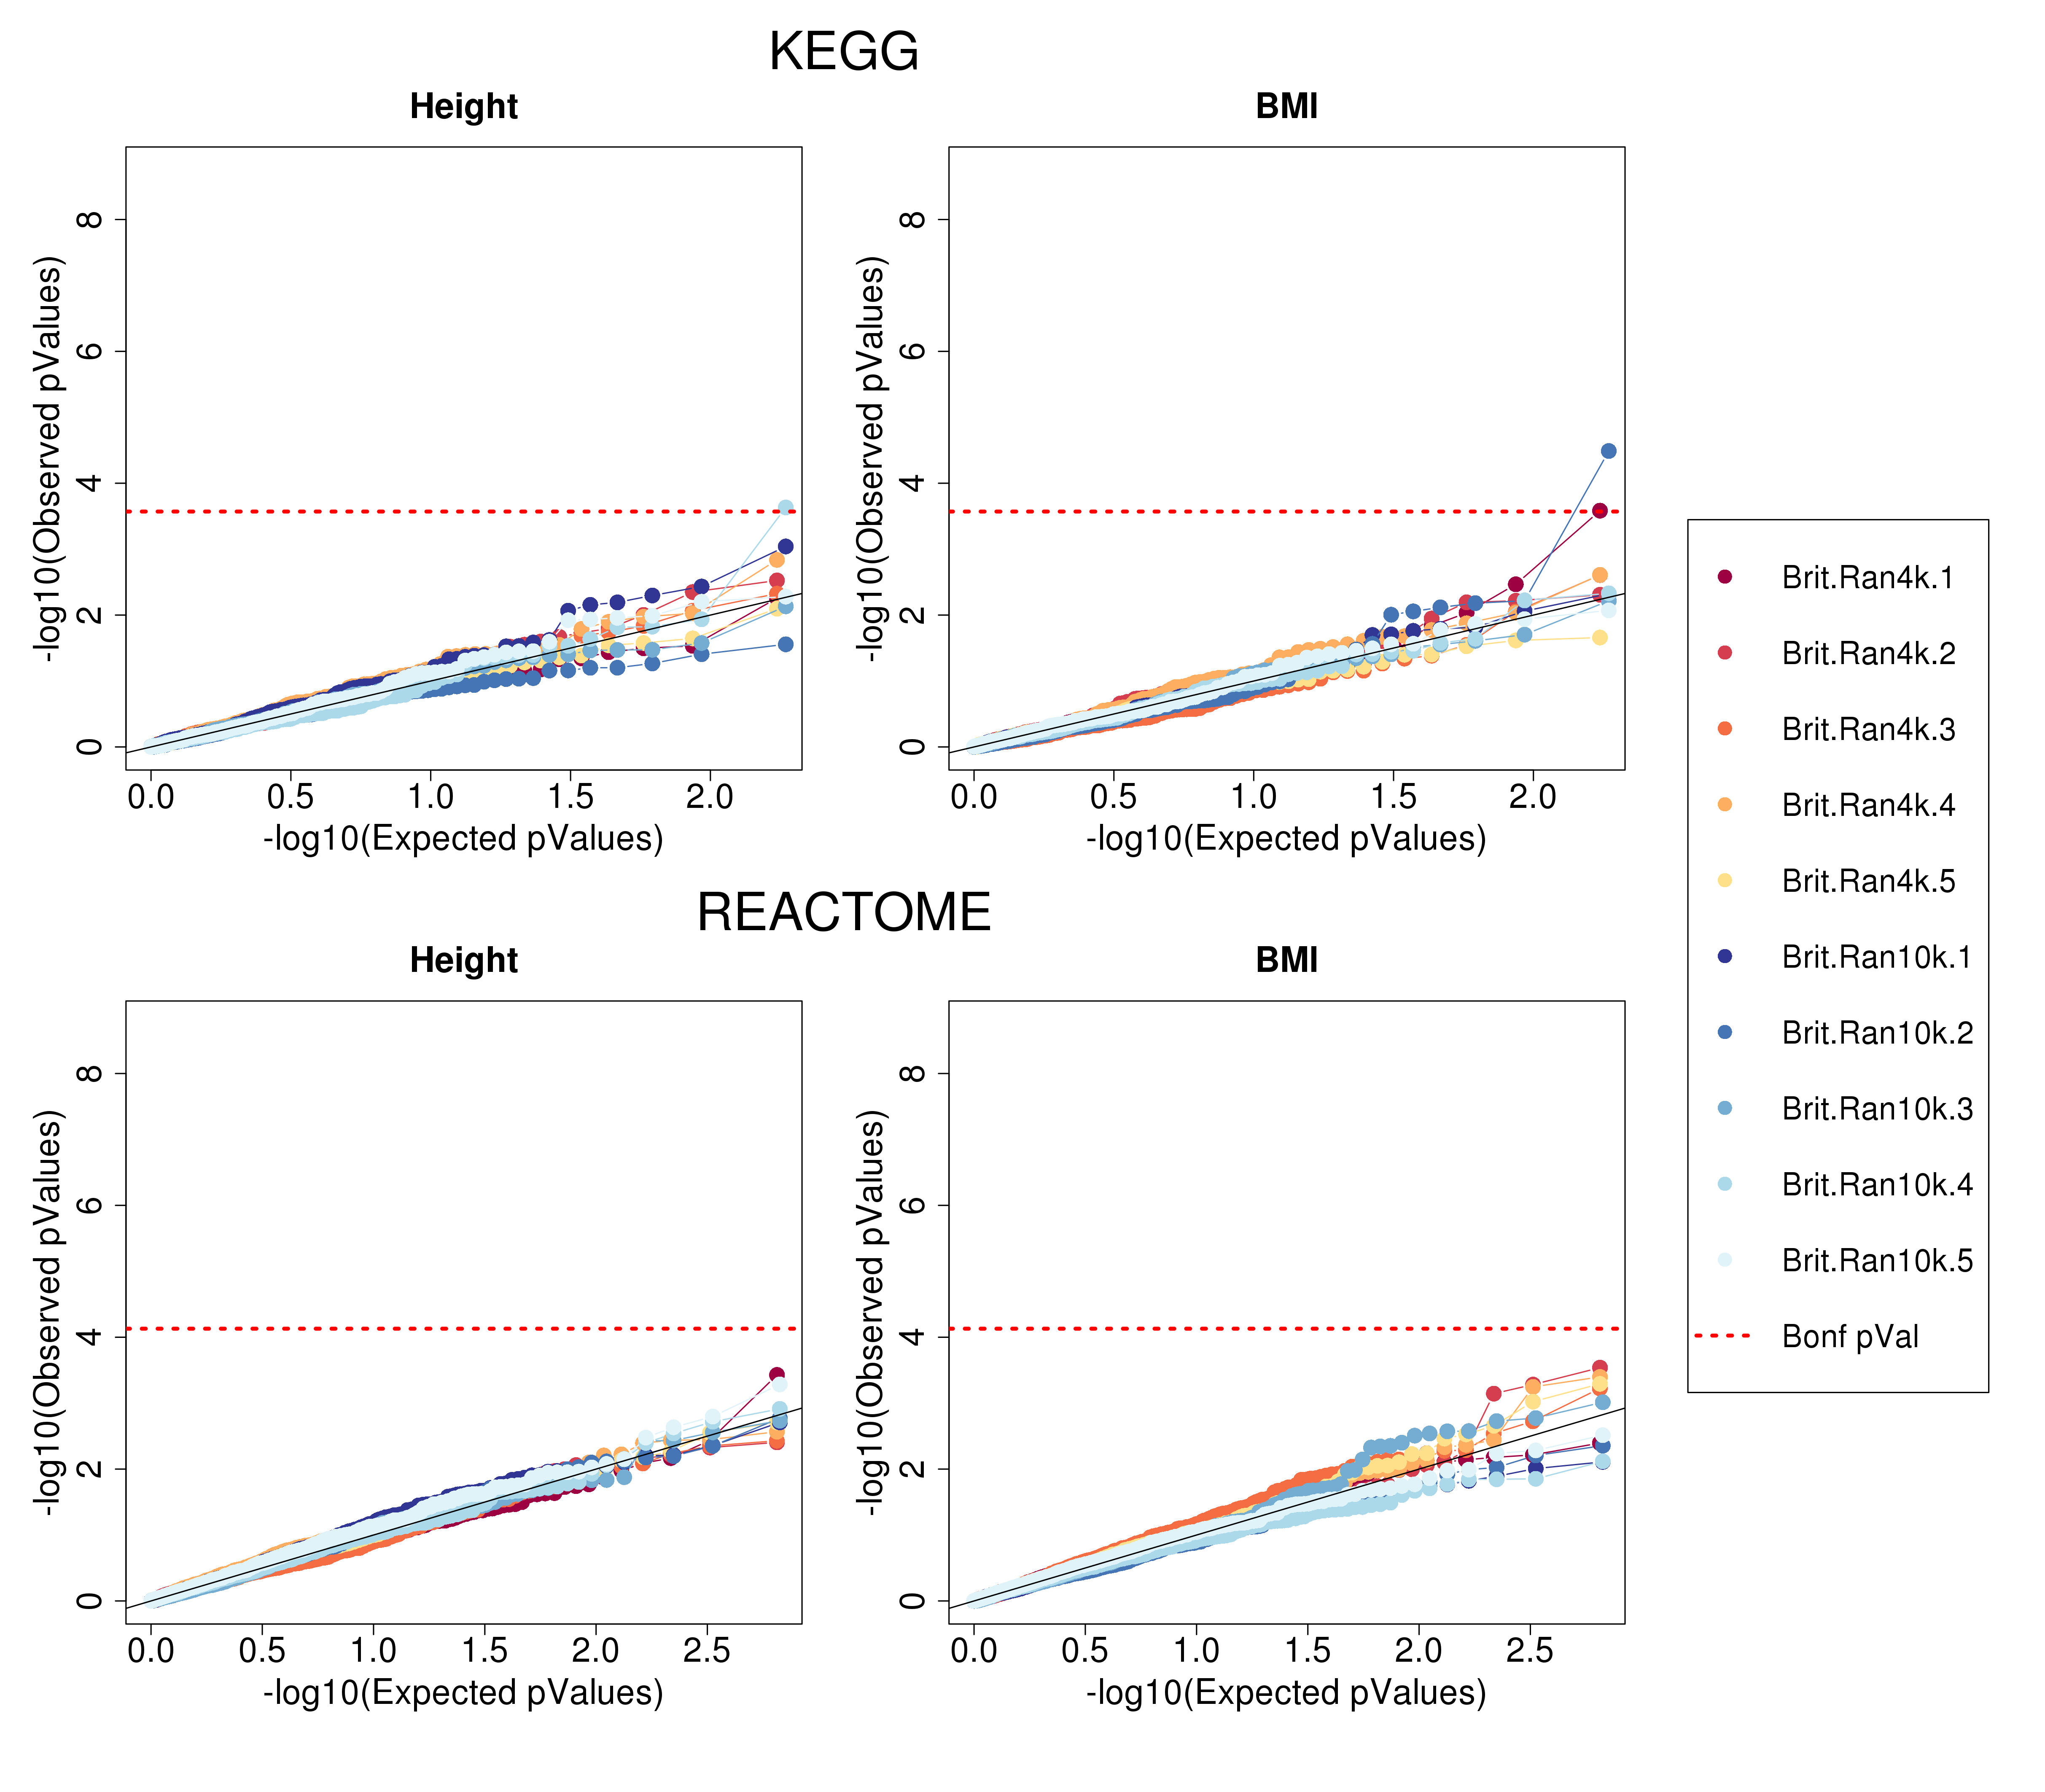
\includegraphics[scale=.35]{Images/Supp/InterPath_Supp_Figure_BritReps_perm1_QQPlots_AllPaths_vs1.png}
\caption[TBD]{\textbf{QQ-Plots of MAPIT-R results using permuted phenotypes, per British replicate}. The figure shows QQ-plots for running MAPIT-R using single, permuted versions of both height and BMI with the KEGG \& REACTOME databases. Phenotypes were permuted within each British replicate subgroup. Shown on the $x$-axis are the -$\log_{10}$ of the expected $p$-values and the on the $y$-axis are on the -$\log_{10}$ of the observed $p$-values. The dotted red line is the Bonferroni-corrected $p$-value threshold based on the number of pathways tested per pathway database-phenotype combination. We find across all pathway database-phenotype-replicate combinations that MAPIT-R continues to show proper null behavior within the range expected when using permuted phenotypes.}
\label{InterPath-Supp-Figure-BritReps-perm1-QQPlots-AllPaths}
\end{figure}
\clearpage

%\newcounter{CharNumber3}
%\setcounter{CharNumber3}{1}
%\renewcommand{\thefigure}{\arabic{figure}\alph{CharNumber3}}
\setlength{\footskip}{1cm}
\begin{figure}[htbp]
\centering
\vspace*{-1cm}
\includegraphics[scale=.2]{Images/Supp/InterPath_Supp_Figure_BritReps_pValHists_AllPaths_vs1_pt1.png}
\caption[TBD]{\textbf{$p$-Value histograms of MAPIT-R results using permuted phenotypes, per British replicate}. The figure shows histograms of MAPIT-R $p$-values collected across ten independent phenotype permutation runs for each British Ran4000 and Ran10000 subsample replicate. The same phenotype permutation for a given replicate was used across both pathway databases (i.e. 10 permutations were done for height and 10 done for BMI for each subgroup). Covariates used from the original MAPIT-R analysis were kept the same.}
\label{InterPath-Supp-Figure-BritReps-10perms-pValHists-pt1}
\end{figure}
\clearpage
\setlength{\footskip}{1cm}
\addtocounter{figure}{-1}
%\addtocounter{CharNumber3}{1}

\setlength{\footskip}{2cm}
\begin{figure}[htbp]
\centering
\vspace*{-1cm}
\includegraphics[scale=.2]{Images/Supp/InterPath_Supp_Figure_BritReps_pValHists_AllPaths_vs1_pt2.png}
\caption[TBD]{\textbf{$p$-Value histograms of MAPIT-R results using permuted phenotypes, per British replicate}. The figure shows histograms of MAPIT-R $p$-values collected across ten independent phenotype permutation runs for each British Ran4000 and Ran10000 subsample replicate. The same phenotype permutation for a given replicate was used across both pathway databases (i.e. 10 permutations were done for height and 10 done for BMI for each subgroup). Covariates used from the original MAPIT-R analysis were kept the same.}
\label{InterPath-Supp-Figure-BritReps-10perms-pValHists-pt2}
\end{figure}
\clearpage
\setlength{\footskip}{1cm}
%\renewcommand{\thefigure}{\arabic{figure}}

\setlength{\footskip}{3cm}
\begin{figure}[htbp]
\centering
\vspace*{-2cm}
\includegraphics[scale=.2]{Images/Supp/InterPath_Supp_Figure_pValsVsNumSNPs_vs3.png}
\caption[TBD]{\textbf{Number of SNPs in a pathway versus a pathway's MAPIT-R $p$-value}. Caption continued on next page.}
\label{InterPath-Supp-Figure-pValsVsNumSNPs}
\end{figure}
\clearpage
\setlength{\footskip}{1cm}

\addtocounter{figure}{-1}
\begin{figure} [t!]
  \caption{\textbf{Number of SNPs in a pathway versus a pathway's MAPIT-R $p$-value}. The figure shows plots comparing the MAPIT-R $p$-values from our main analysis to the number of SNPs present in each pathway. Results for every pathway database-phenotype-UB subgroup combinations are shown. The dotted red line is the line of best fit and the legend provides the regression coefficient and its associated $p$-value. We observe that for most combinations there is a significant relationship between MAPIT-R $p$-value and the number of SNPs present in a pathway. This follows our hypothesis that combining SNPs together in a joint analysis might provide greater power to detect marginal epistasis than analyzing each SNP independently. We note, however, that these results appear to not solely be driven just by the presence or absence of large SNP counts -- conducting this same analysis on one of our sets of permuted phenotypes we now find very few significant relationships between MAPIT-R $p$-values and pathway SNP counts (Supplementary Figure \ref{InterPath-Supp-Figure-pValsVsNumSNPs-perm1}).}
\label{InterPath-Supp-Figure-pValsVsNumSNPs-Caption}
\end{figure}
\clearpage

\setlength{\footskip}{3cm}
\begin{figure}[htbp]
\centering
\vspace*{-2cm}
\includegraphics[scale=.2]{Images/Supp/InterPath_Supp_Figure_pValsVsNumSNPs_perm1_vs3.png}
\caption[TBD]{\textbf{Number of SNPs in a pathway versus a pathway's MAPIT-R $p$-value using permuted phenotypes}. Caption continued on next page.}
\label{InterPath-Supp-Figure-pValsVsNumSNPs-perm1}
\end{figure}
\clearpage
\setlength{\footskip}{1cm}

\addtocounter{figure}{-1}
\begin{figure} [t!]
  \caption{\textbf{Number of SNPs in a pathway versus a pathway's MAPIT-R $p$-value using permuted phenotypes}. The figure shows plots comparing the MAPIT-R $p$-values from our main analysis to the number of SNPs present in each pathway. For this analysis a single set of our permuted phenotypes (i.e. Supplementary Figure \ref{InterPath-Supp-Figure-perm1-QQPlots-AllPaths}) was used for each UKB subgroup. Results for every pathway database-phenotype-subgroup combination is shown. The dotted red line is the line of best fit and the legend provides the regression coefficient and its associated $p$-value. We observe that for very few combinations there is any relationship between MAPIT-R $p$-value and the number of SNPs present in a pathway. For the same analysis on the original set of observed phenotypes, see Supplementary Figure \ref{InterPath-Supp-Figure-pValsVsNumSNPs}.}
\label{InterPath-Supp-Figure-pValsVsNumSNPs-perm1-Caption}
\end{figure}
\clearpage

%\begin{figure}[htb]
%\centering
%\hspace*{-1.4cm}
%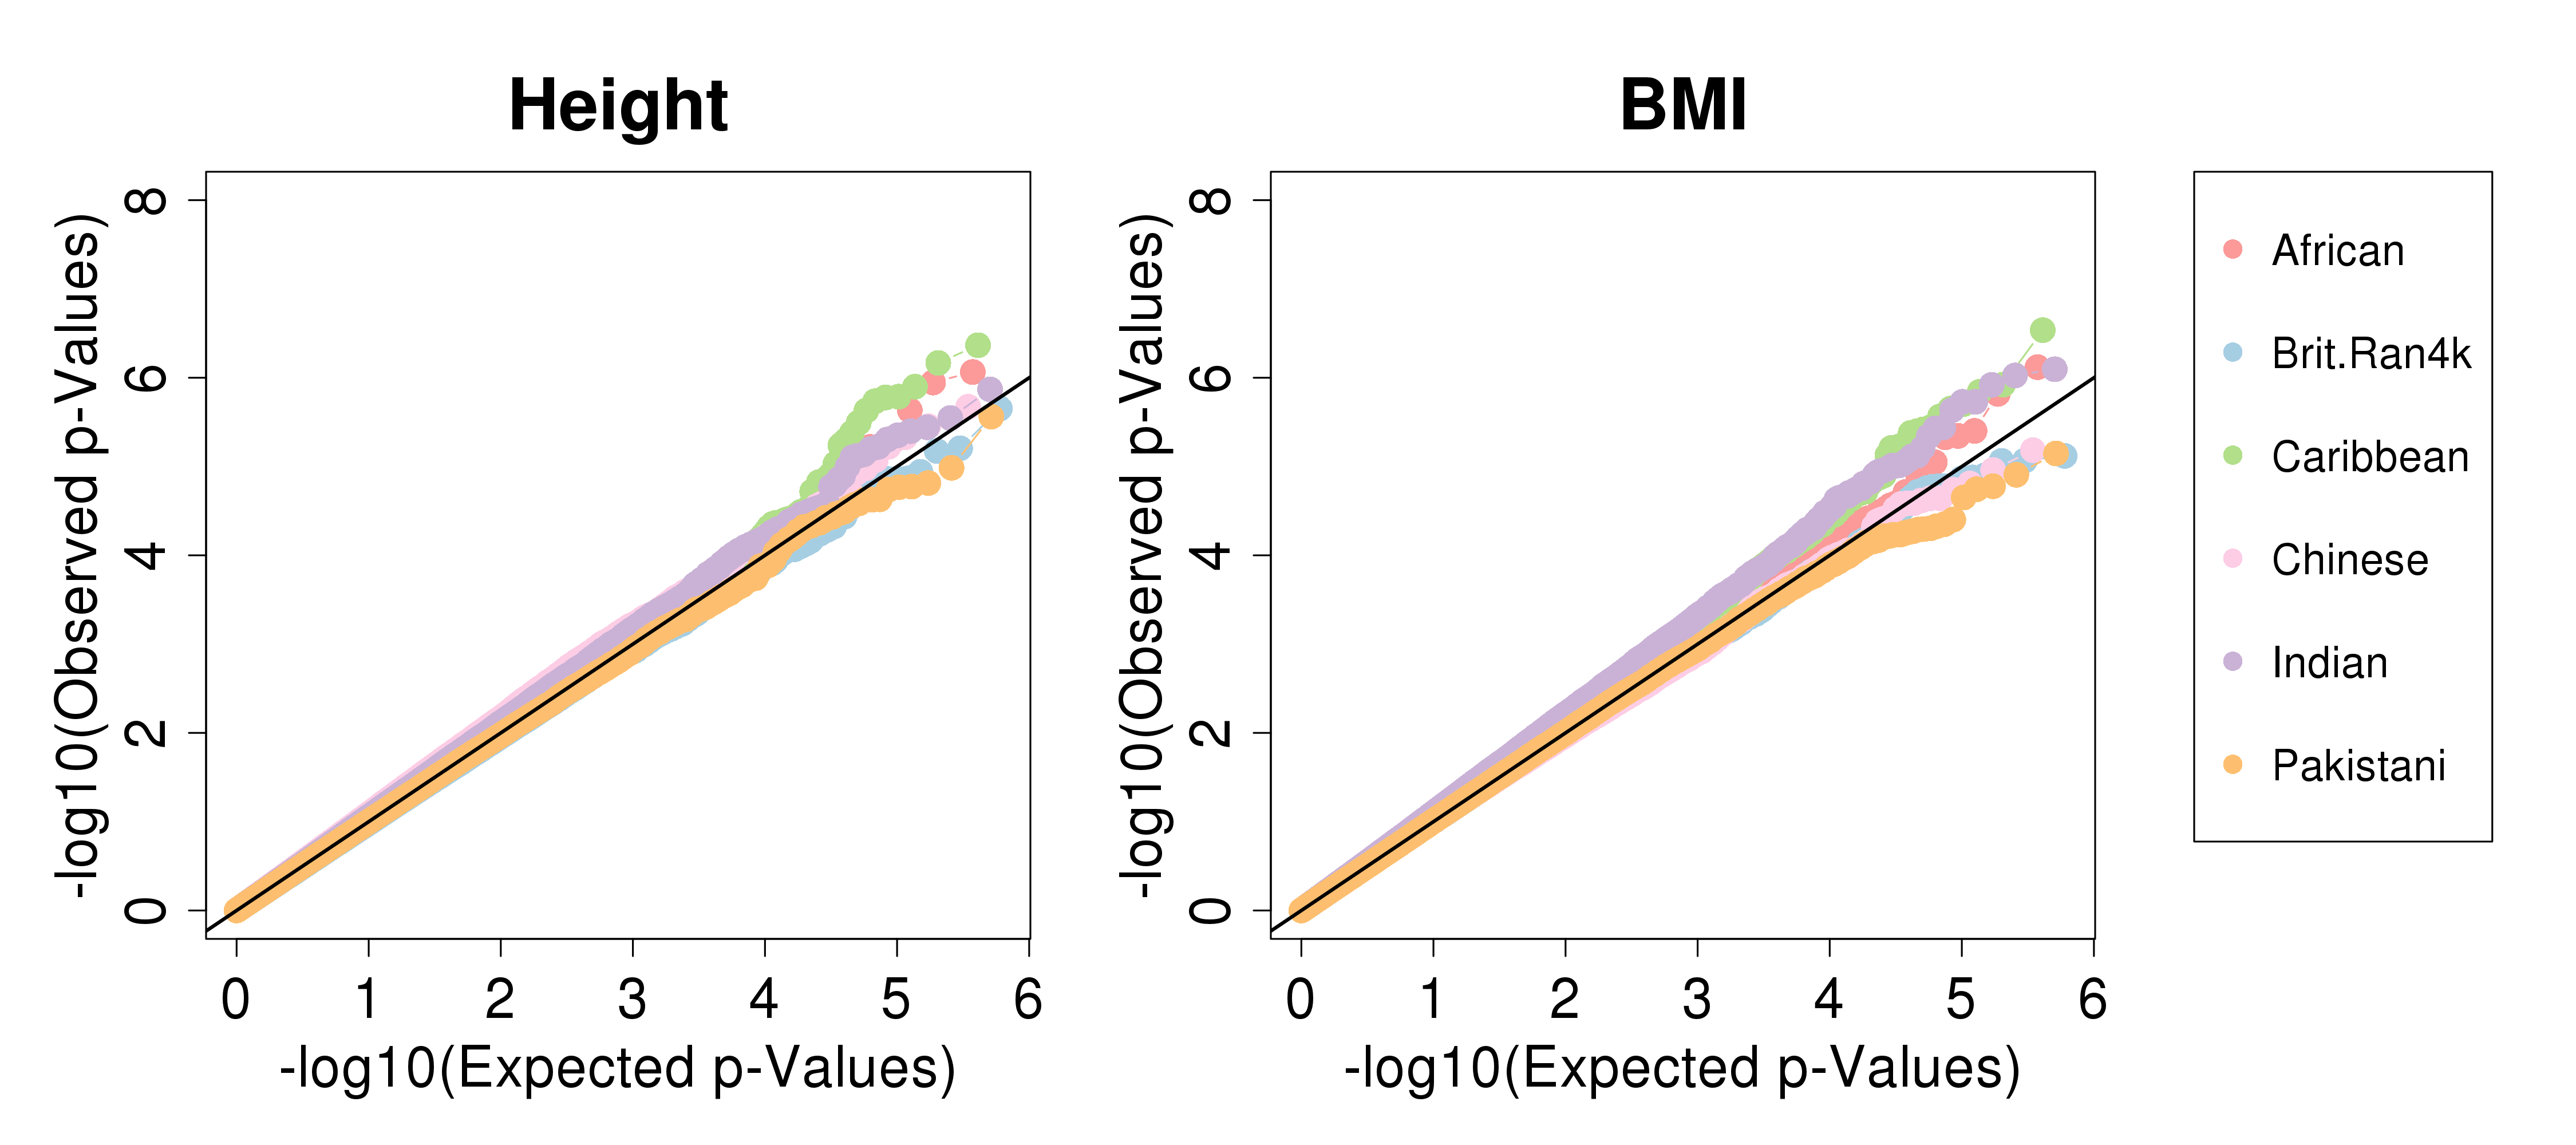
\includegraphics[scale=.45]{Images/Main/InterPath_Main_Figure_MAPIT_vs4_HeightBMI.png}
%\caption[TBD]{\textbf{QQ-Plots of MAPIT results, per subgroup}. The figure shows QQ-plots of our results from running MAPIT on our four initial UKB population subgroups in height and BMI. On the $x$-axis are the -$\log_{10}$ of the expected $p$-values and the on the $y$-axis are on the -$\log_{10}$ of the observed $p$-values. Each data point is a SNP and total SNP counts per UKB subgroup can be found in Supplementary Table \ref{InterPath-Supp-Table-UKBPopStats}. We observe no genome-wide significant signals in any subgroup across both phenotypes ($p$-value $< 5\times10^{-8}$) and, due to this lack of significant results, observe no clear differences in patterns between our subgroups.}
%\label{InterPath-Supp-Figure-MAPIT-HeightBMI}
%\end{figure}

%\begin{figure}[htbp]
%\centering
%\hspace*{-1.7cm}
%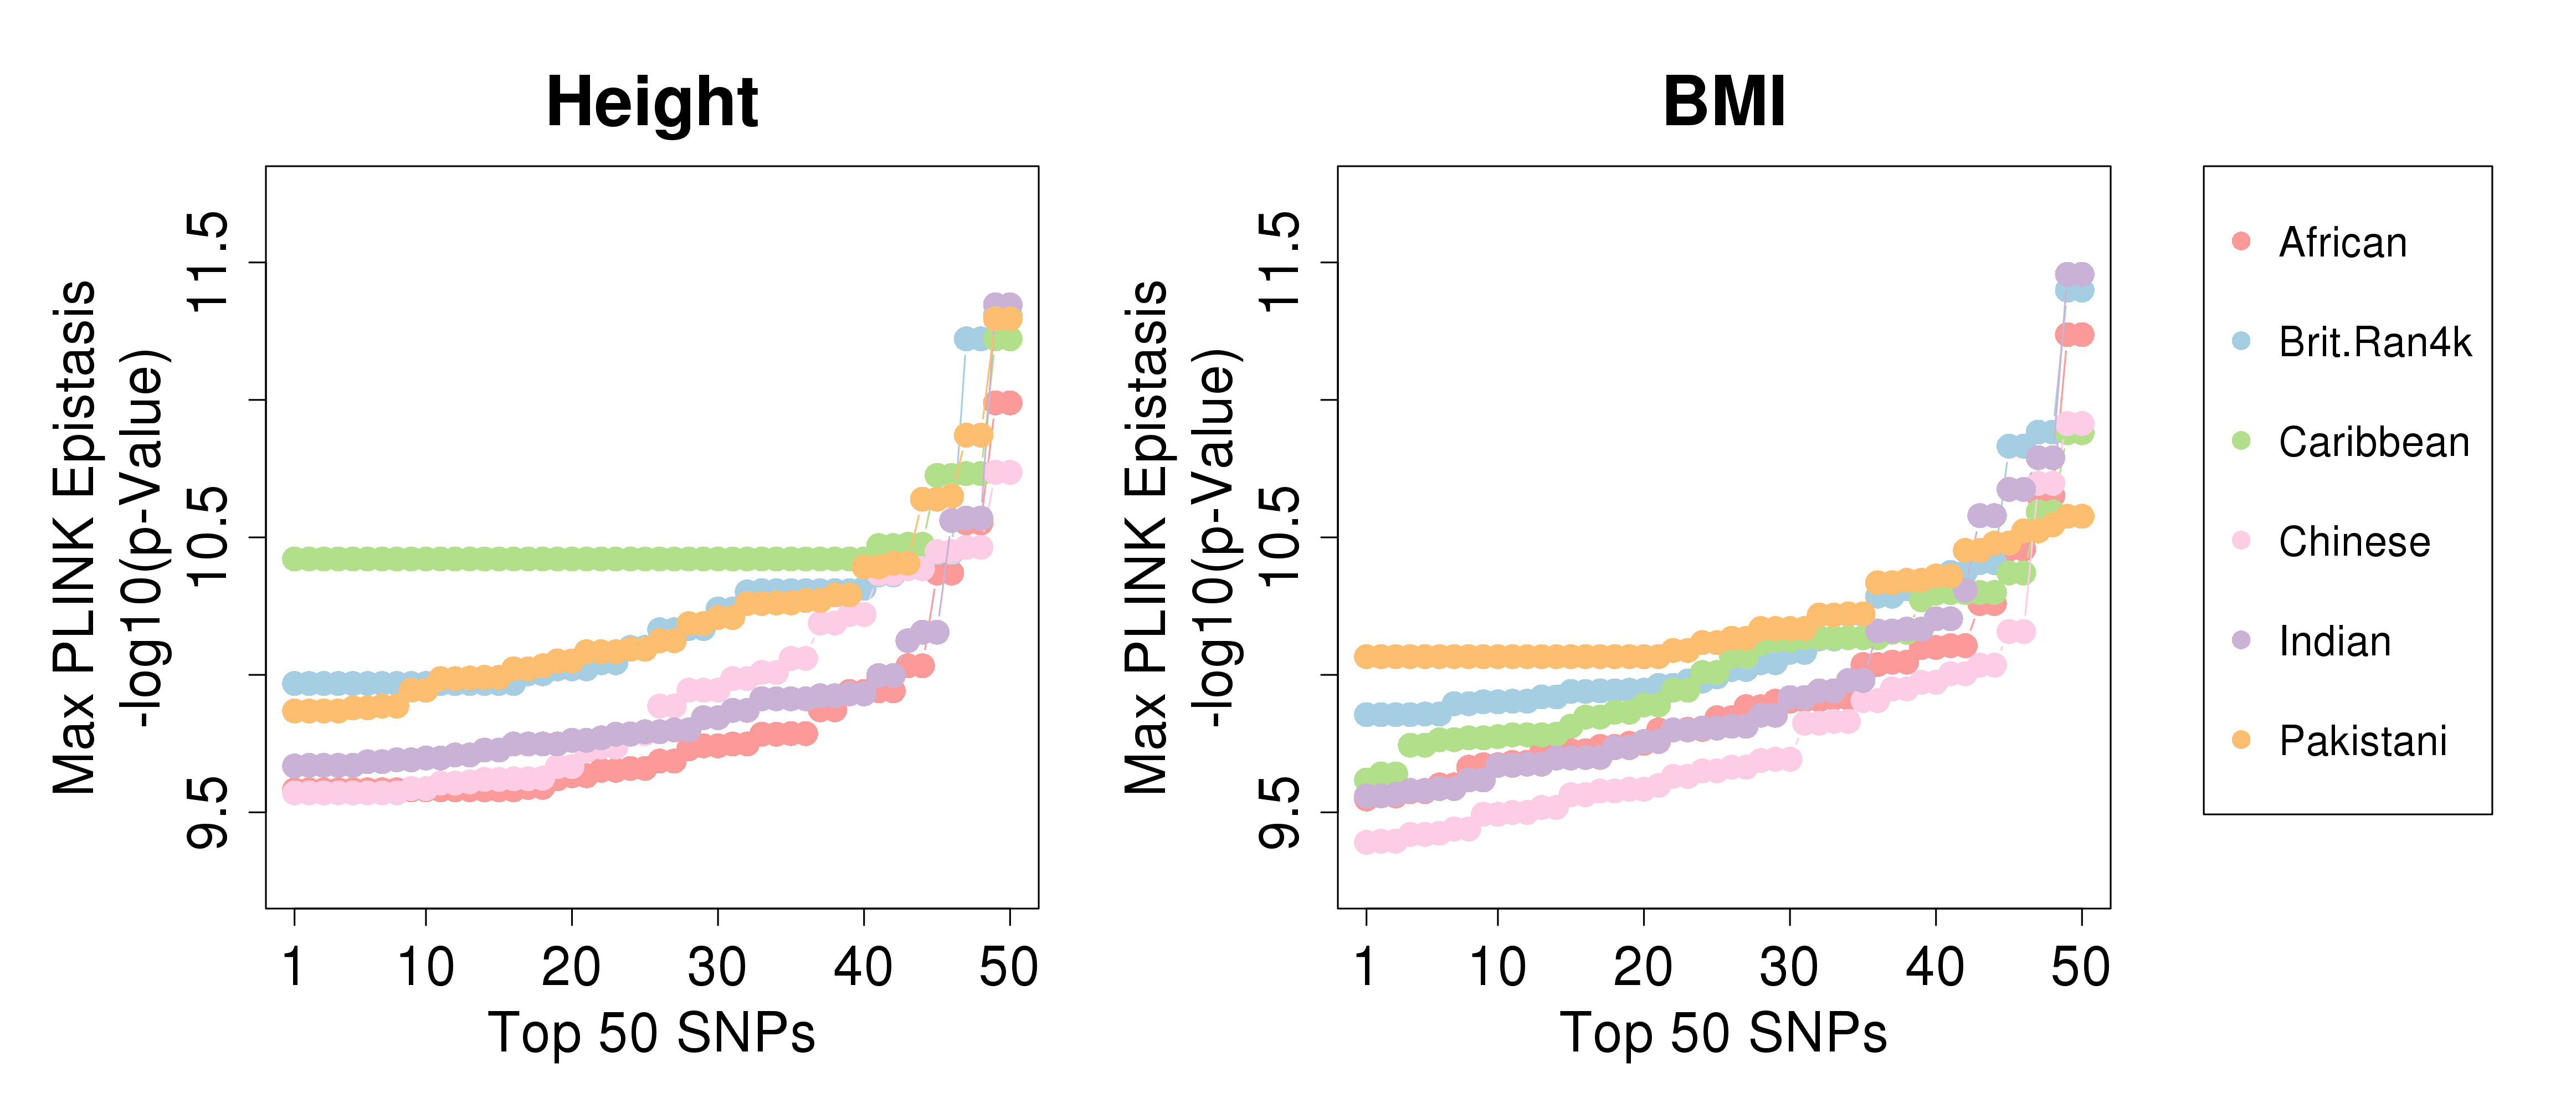
\includegraphics[scale=.45]{Images/Supp/InterPath_Supp_Figure_PLINK_BestSNPs_vs2_AllPops_HeightBMI.png}
%\caption[TBD]{\textbf{SNPs with the largest PLINK pairwise epistasis signals, per subgroup}. The figure shows the best $p$-values obtained from running PLINK's exhaustive pairwise SNP epistasis test for both height and BMI in each of the UKB subgroups. Only the top 50 SNPs, sorted by best pairwise SNP epistasis $p$-value, for each subgroup are shown. No test reaches genome-wide significance based on using a Bonferroni-corrected $p$-value threshold ($p$-value $< 5\times10^{-13}$).}
%\label{InterPath-Supp-Figure-PLINK-HeightBMI-AllPops}
%\end{figure}
%\clearpage

%From: ,https://tex.stackexchange.com/questions/64934/subfig-label-positioning, https://tex.stackexchange.com/questions/196653/how-do-i-stack-two-figures-on-top-of-each-other-rather-than-side-to-side, https://tex.stackexchange.com/questions/47311/include-table-as-a-subfigure, https://tex.stackexchange.com/questions/169541/looking-for-three-images-on-top-of-each-other-with-text-underneath-each, https://tex.stackexchange.com/questions/10863/is-there-a-way-to-slightly-shrink-a-table-including-font-size-to-fit-within-th

\newcounter{CharNumber5}
\setcounter{CharNumber5}{1}
\renewcommand{\thefigure}{\arabic{figure}\alph{CharNumber5}}
\begin{figure}[ht]
\centering
\vspace*{-.5cm}
\subfloat[]{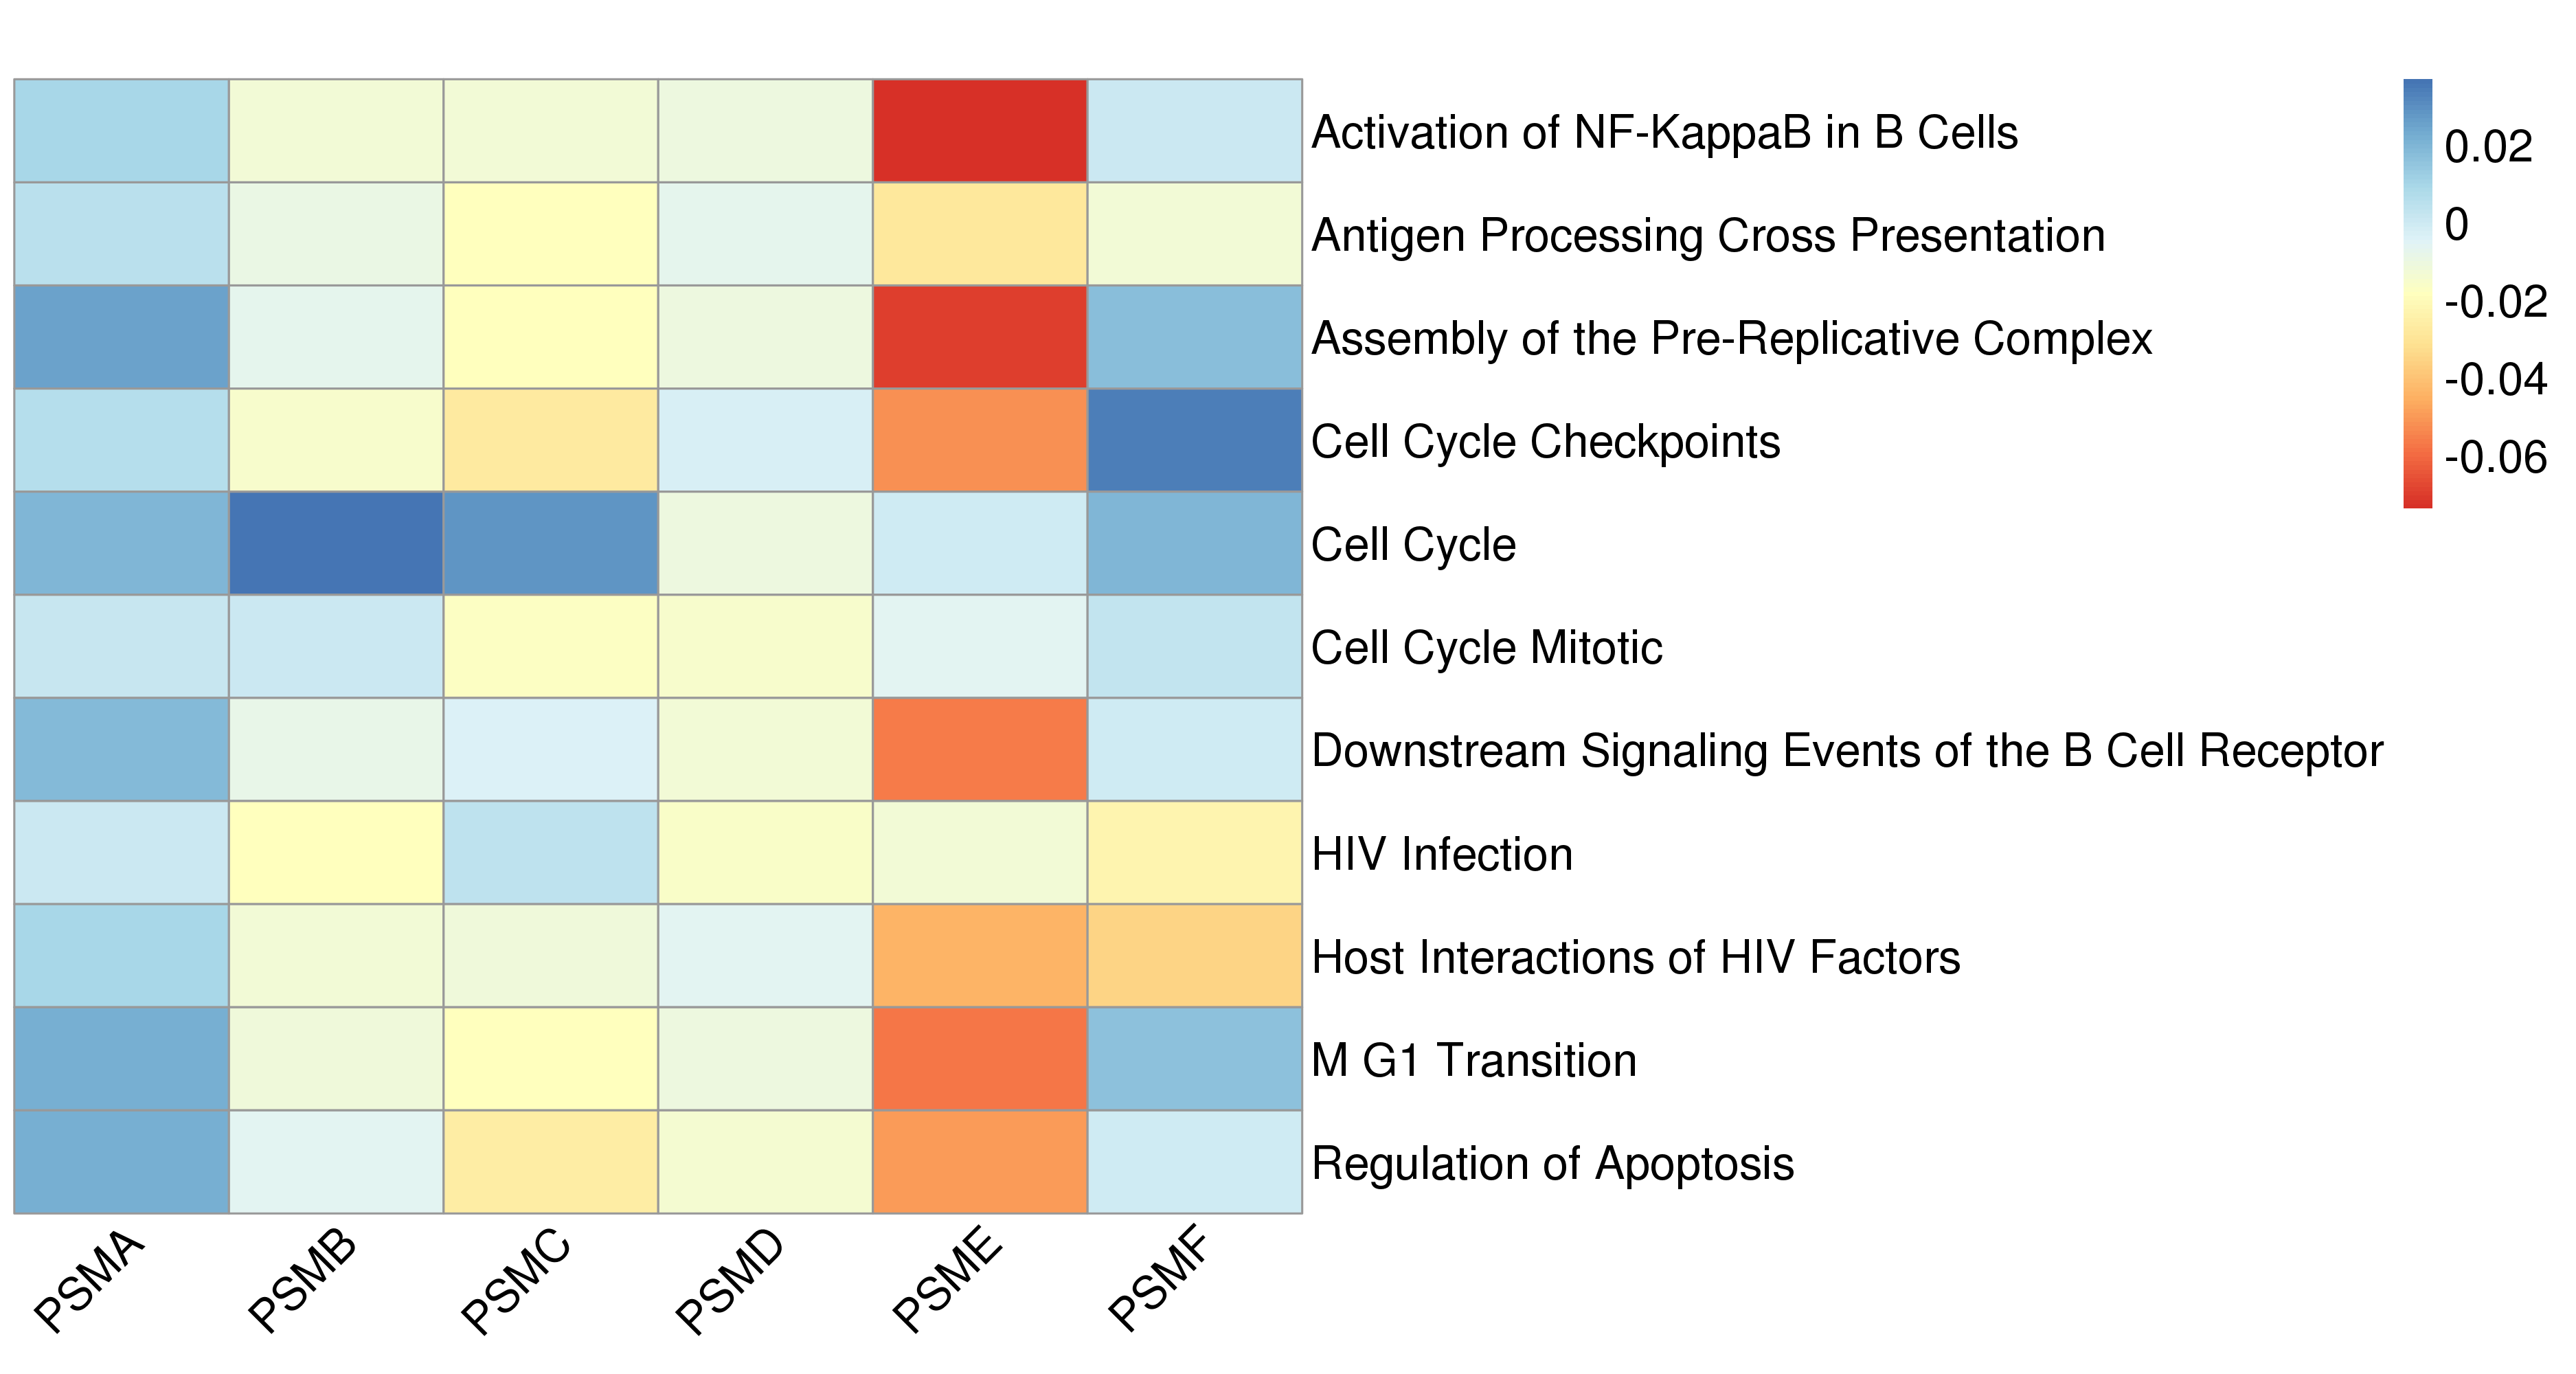
\includegraphics[scale=.5]{Images/Supp/InterPath_Supp_Figure_Proteaseome_Heatplots_African_Loop_vs3.png}}
\par
\subfloat[]{\resizebox{1.1\columnwidth}{!}{
 \hspace*{-1.75cm}
 \begin{tabular}{cc|ccc}
  \hline
\textbf{Proteasome} & \textbf{SNPs} & \textbf{REACTOME} & \textbf{SNPs} & \textbf{MAPIT-R} \\
 \textbf{Gene Family} & & \textbf{Pathway} & & \textbf{$p$-Value} \\
  \hline
PSMA & 17 & Activation of NF-KappaB in B Cells & 465 & 1.86E-05  \\
PSMB & 74 & Antigen Processing Cross Presentation & 850 & 3.96E-05 \\
PSMC & 20 & Assembly of the Pre-Replicative Complex & 331 & 3.29E-05 \\
PSMD & 62 & Cell Cycle Checkpoints & 670 & 5.78E-06 \\
PSME & 15 & Cell Cycle & 2459 & 1.29E-06 \\
PSMF & 16 & Cell Cycle Mitotic & 1906 & 4.51E-05 \\
 & & Downstream Signaling Events of the B Cell Receptor & 745 & 1.19E-05 \\
 & & HIV Infection & 1346 & 7.53E-07 \\
 & & Host Interactions of HIV Factors & 963 & 7.52E-06 \\
 & & M G1 Transition & 458 & 3.19E-06 \\
 & & Regulation of Apoptosis & 564 & 1.22E-05 \\
  \hline
\end{tabular}}}
\caption[TBD]{\textbf{Proteasome gene family leave-one-out MAPIT-R reruns, REACTOME-BMI-African}. (a) The figure shows the change in original MAPIT-R -$\log_{10}$ $p$-value for each presented REACTOME pathway when each proteasome gene family is removed one at a time. The analyses were conducted in the BMI-African subgroup combination. The $x$-axis shows each proteasome gene family and the $y$-axis shows each REACTOME pathway. Each column has been scaled by the number of SNPs present in the given gene family and, as a result, the heatplot specifically shows the -$\log_{10}$ $p$-value change per SNP. (b) The table shows the number of SNPs that are present in each proteasome gene family (left) and each REACTOME pathway (right). The original MAPIT-R $p$-values for each pathway are also shown (right).}
\label{InterPath-Supp-Figure-Prot-Heatplots-African}
\end{figure}
\clearpage
\addtocounter{figure}{-1}
\addtocounter{CharNumber5}{1}

%\captionsetup[subfigure]{position=top, labelfont=bf,textfont=normalfont,singlelinecheck=off,justification=raggedright}

\begin{figure}[ht]
\centering
\vspace*{-.5cm}
\subfloat[]{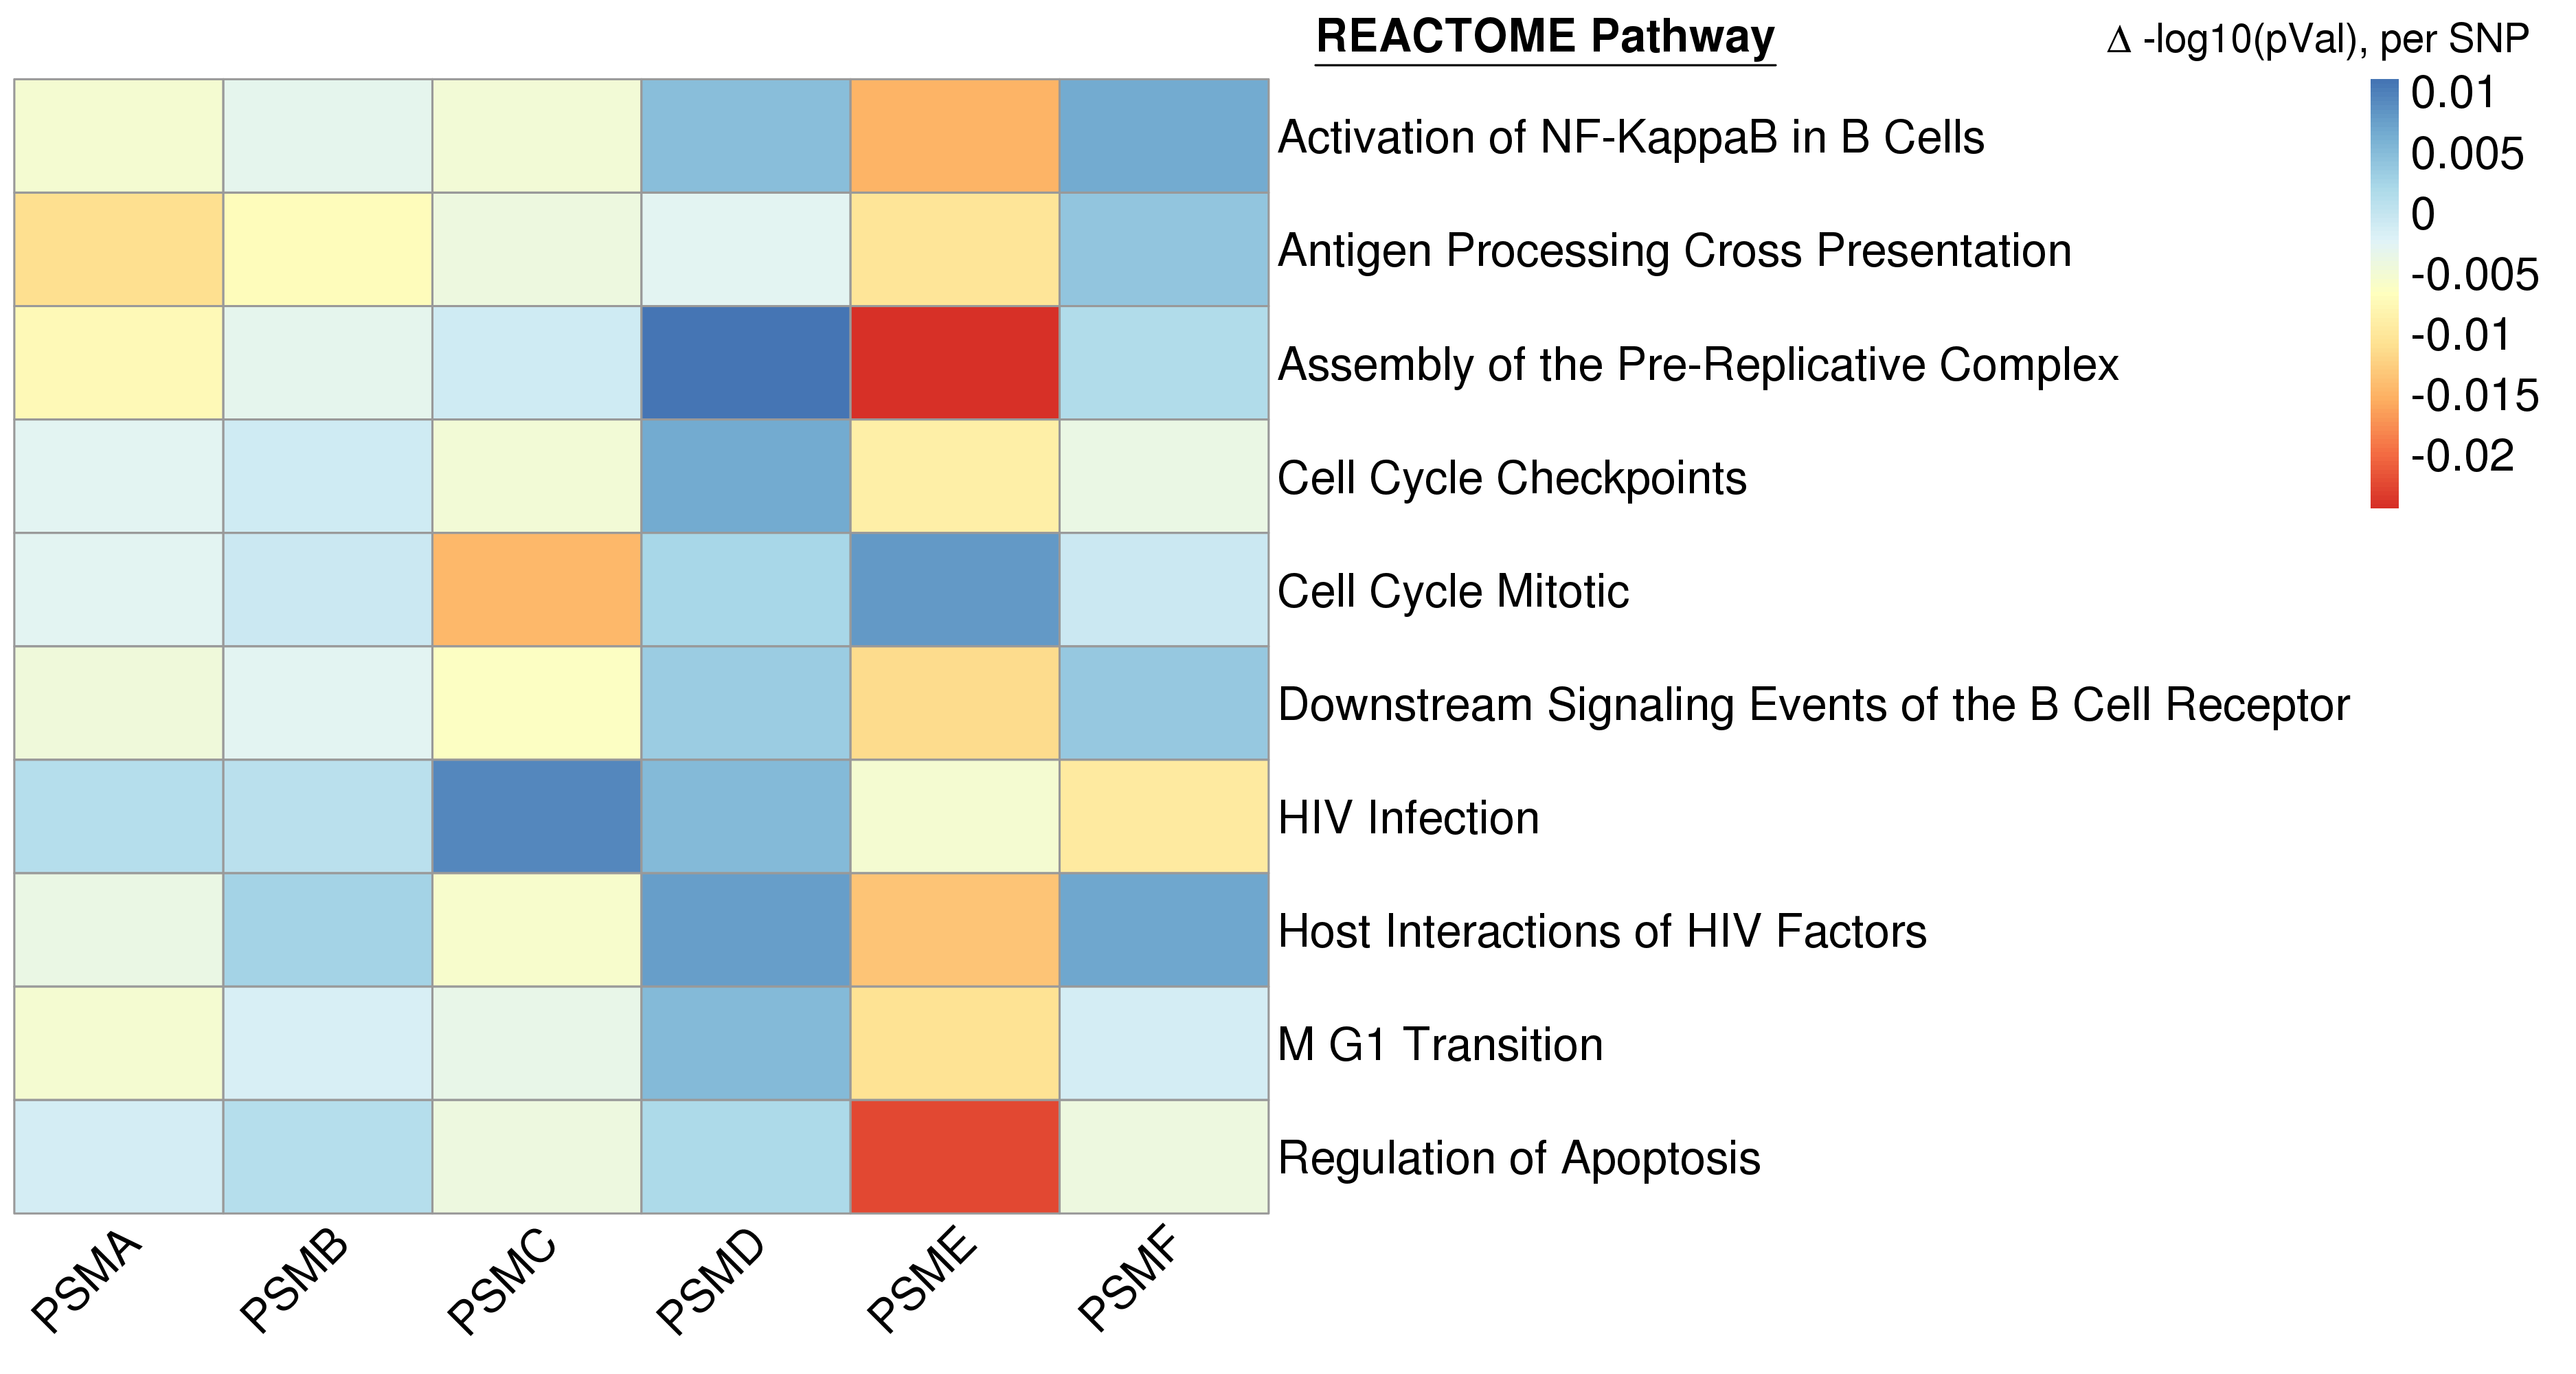
\includegraphics[scale=.5]{Images/Supp/InterPath_Supp_Figure_Proteaseome_Heatplots_BritRan4000_Loop_vs3.png}}
\par
\subfloat[]{\resizebox{1.1\columnwidth}{!}{
 \hspace*{-1.75cm}
 \begin{tabular}{cc|ccc}
  \hline
\textbf{Proteasome} & \textbf{SNPs} & \textbf{REACTOME} & \textbf{SNPs} & \textbf{MAPIT-R} \\
 \textbf{Gene Family} & & \textbf{Pathway} & & \textbf{$p$-Value} \\
  \hline
PSMA & 40 & Activation of NF-KappaB in B Cells & 756 & 2.28E-01  \\
PSMB & 91 & Antigen Processing Cross Presentation & 1104 & 2.48E-05 \\
PSMC & 29 & Assembly of the Pre-Replicative Complex & 507 & 1.84E-02 \\
PSMD & 101 & Cell Cycle Checkpoints & 1121 & 6.77E-02 \\
PSME & 25 & Cell Cycle Mitotic & 3304 & 2.34E-01 \\
 PSMF & 26 & Downstream Signaling Events of the B Cell Receptor & 1248 & 3.25E-01 \\
 & & HIV Infection & 2221 & 8.26E-02 \\
 & & Host Interactions of HIV Factors & 1541 & 1.55E-02 \\
 & & M G1 Transition & 697 & 3.02E-01 \\
 & & Regulation of Apoptosis & 906 & 2.98E-02 \\
  \hline
\end{tabular}}}
\caption[TBD]{\textbf{Proteasome gene family leave-one-out MAPIT-R reruns, REACTOME-BMI-British.Ran4000}. (a) The figure shows the change in original MAPIT-R -$\log_{10}$ $p$-value for each presented REACTOME pathway when each proteasome gene family is removed one at a time. The analyses were conducted in the BMI-British.Ran4000 subgroup combination. The $x$-axis shows each proteasome gene family and the $y$-axis shows each REACTOME pathway. Each column has been scaled by the number of SNPs present in the given gene family and, as a result, the heatplot specifically shows the -$\log_{10}$ $p$-value change per SNP. (b) The table shows the number of SNPs that are present in each proteasome gene family (left) and each REACTOME pathway (right). The original MAPIT-R $p$-values for each pathway are also shown (right).}
\label{InterPath-Supp-Figure-Prot-Heatplots-BritRan4000}
\end{figure}
\clearpage
\addtocounter{figure}{-1}
\addtocounter{CharNumber5}{1}

\begin{figure}[ht]
\centering
\vspace*{-.5cm}
\subfloat[]{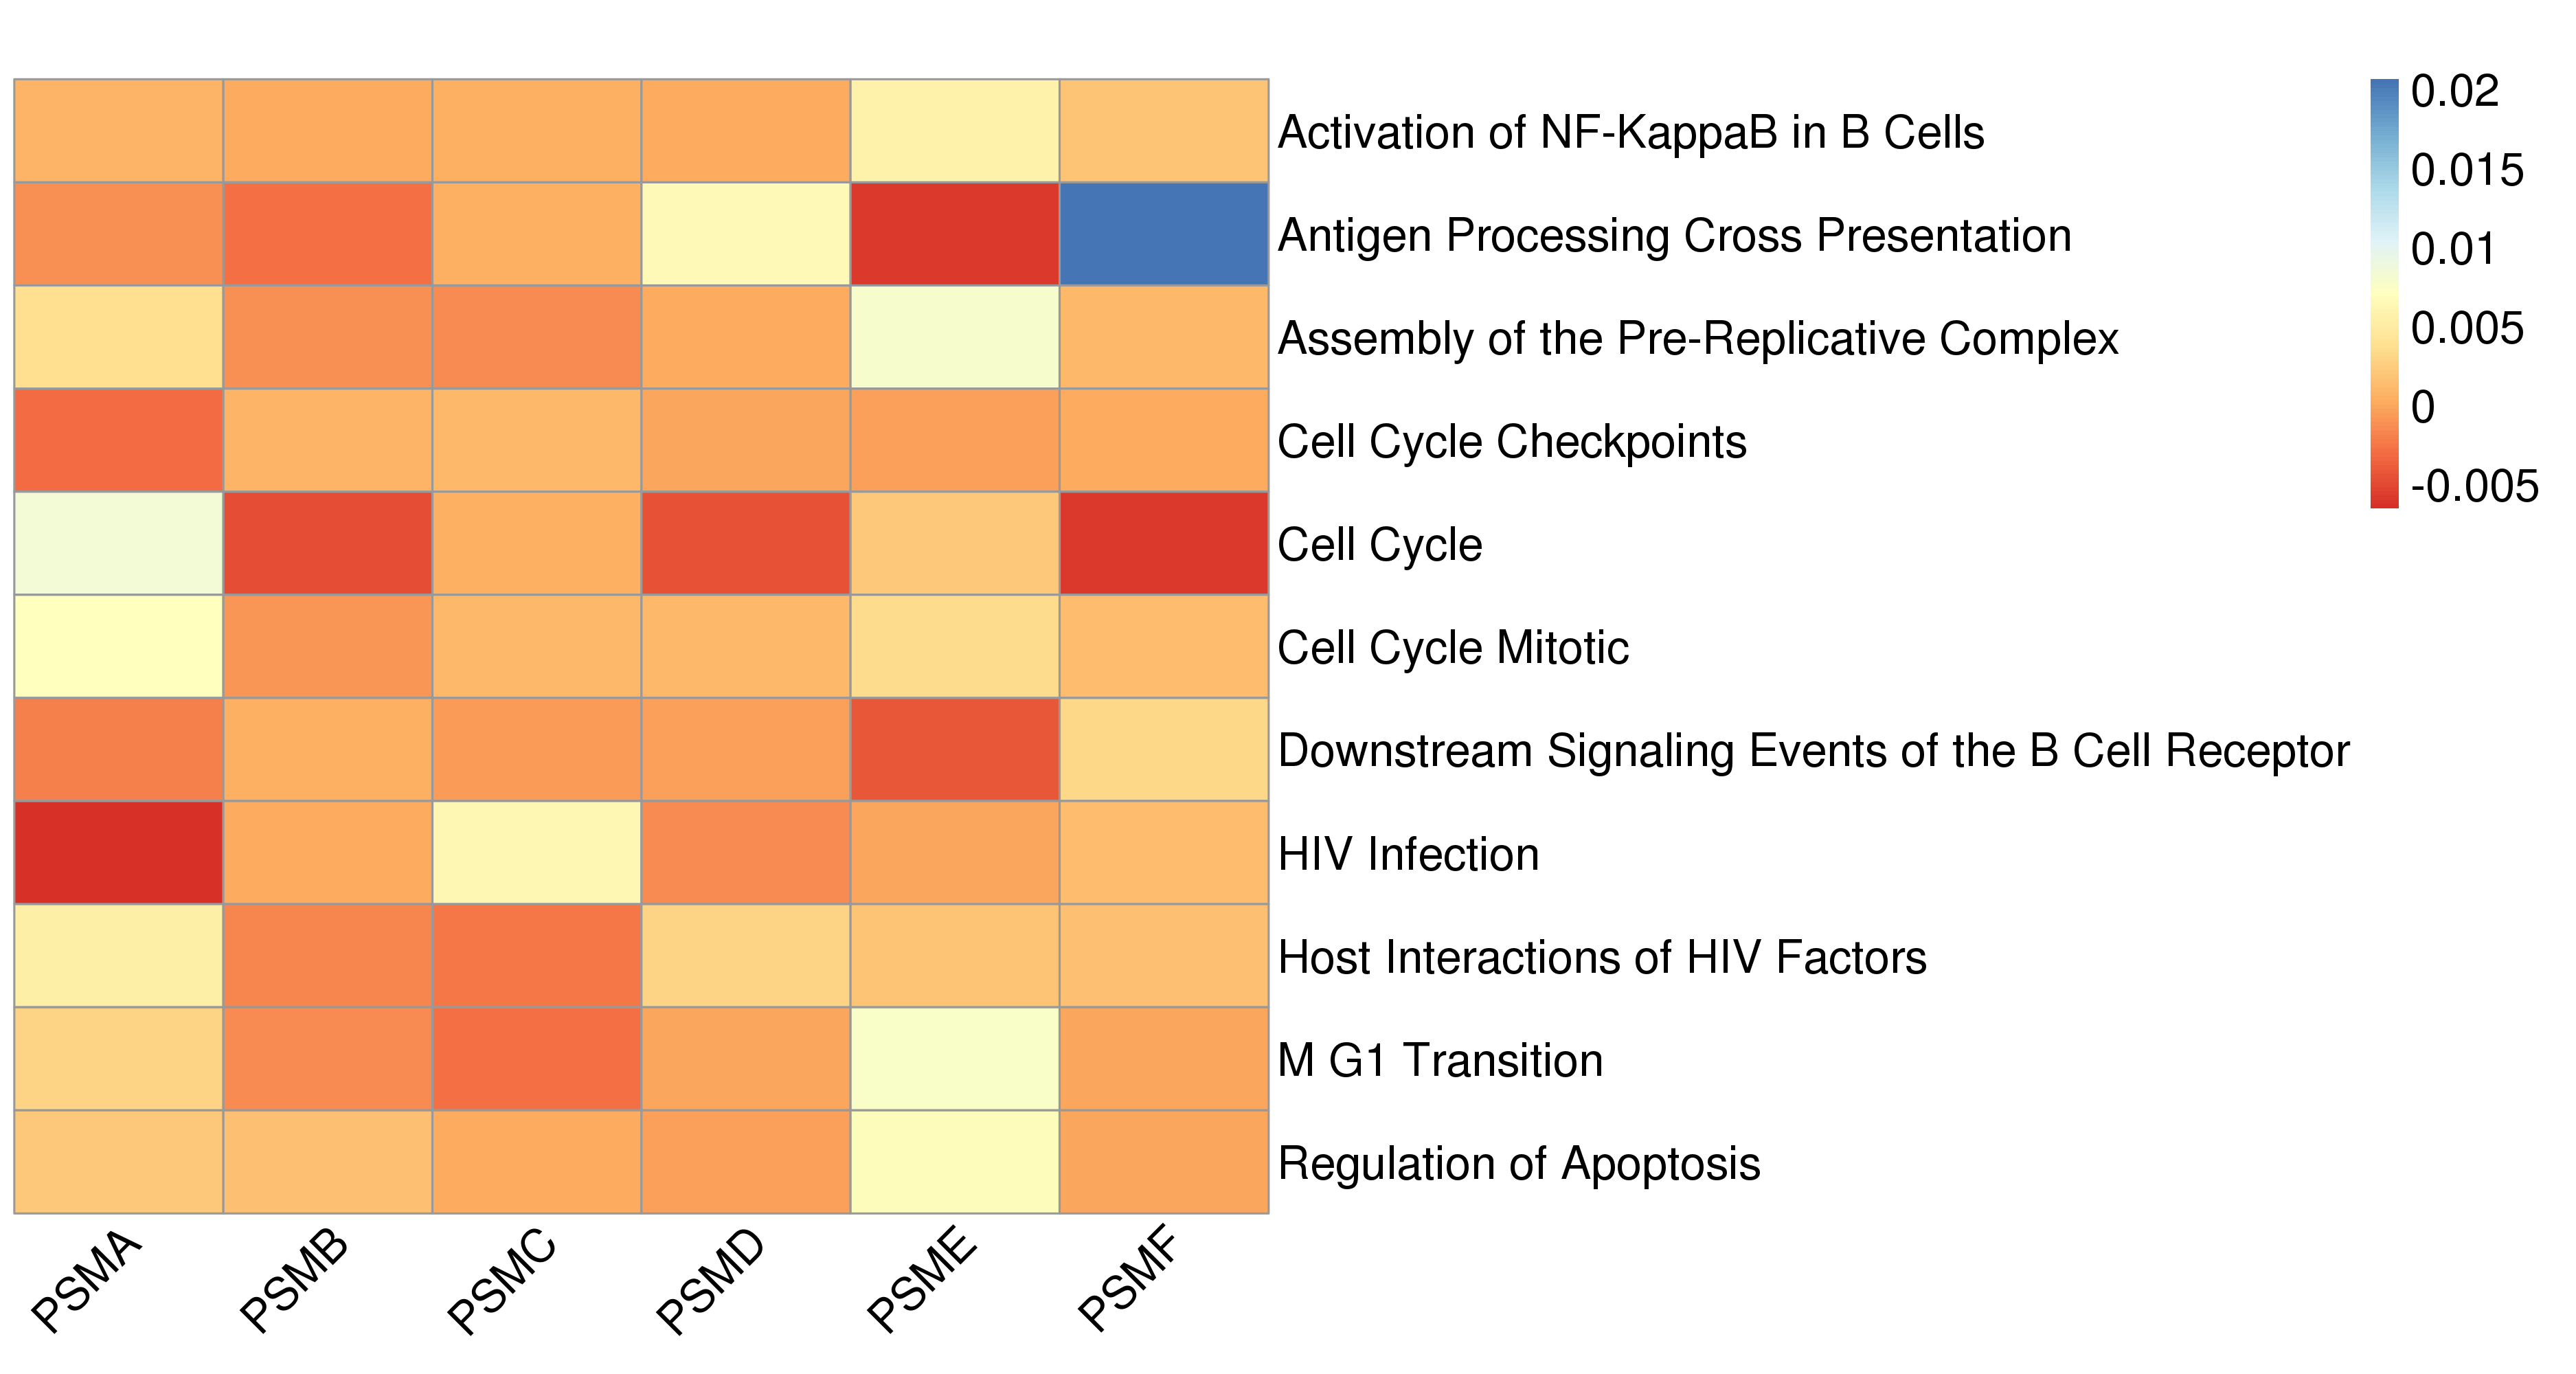
\includegraphics[scale=.5]{Images/Supp/InterPath_Supp_Figure_Proteaseome_Heatplots_Caribbean_Loop_vs3.png}}
\par
\subfloat[]{\resizebox{1.1\columnwidth}{!}{
 \hspace*{-1.75cm}
 \begin{tabular}{cc|ccc}
  \hline
\textbf{Proteasome} & \textbf{SNPs} & \textbf{REACTOME} & \textbf{SNPs} & \textbf{MAPIT-R} \\
 \textbf{Gene Family} & & \textbf{Pathway} & & \textbf{$p$-Value} \\
  \hline
PSMA & 18 & Activation of NF-KappaB in B Cells & 507 & 9.93E-01  \\
PSMB & 77 & Antigen Processing Cross Presentation & 871 & 5.15E-02 \\
PSMC & 21 & Assembly of the Pre-Replicative Complex & 357 & 7.25E-01 \\
PSMD & 69 & Cell Cycle Checkpoints & 736 & 8.83E-01 \\
PSME & 15 & Cell Cycle & 2711 & 2.51E-01 \\
PSMF & 16 & Cell Cycle Mitotic & 2111 & 7.98E-01 \\
 & & Downstream Signaling Events of the B Cell Receptor & 829 & 8.37E-01 \\
 & & HIV Infection & 1483 & 3.11E-01 \\
 & & Host Interactions of HIV Factors & 1055 & 6.68E-01 \\
 & & M G1 Transition & 500 & 6.37E-01 \\
 & & Regulation of Apoptosis & 615 & 9.42E-01 \\
  \hline
\end{tabular}}}
\caption[TBD]{\textbf{Proteasome gene family leave-one-out MAPIT-R reruns, REACTOME-BMI-Caribbean}. (a) The figure shows the change in original MAPIT-R -$\log_{10}$ $p$-value for each presented REACTOME pathway when each proteasome gene family is removed one at a time. The analyses were conducted in the BMI-Caribbean subgroup combination. The $x$-axis shows each proteasome gene family and the $y$-axis shows each REACTOME pathway. Each column has been scaled by the number of SNPs present in the given gene family and, as a result, the heatplot specifically shows the -$\log_{10}$ $p$-value change per SNP. (b) The table shows the number of SNPs that are present in each proteasome gene family (left) and each REACTOME pathway (right). The original MAPIT-R $p$-values for each pathway are also shown (right).}
\label{InterPath-Supp-Figure-Prot-Heatplots-Caribbean}
\end{figure}
\clearpage
\addtocounter{figure}{-1}
\addtocounter{CharNumber5}{1}

\begin{figure}[ht]
\centering
\vspace*{-.5cm}
\subfloat[]{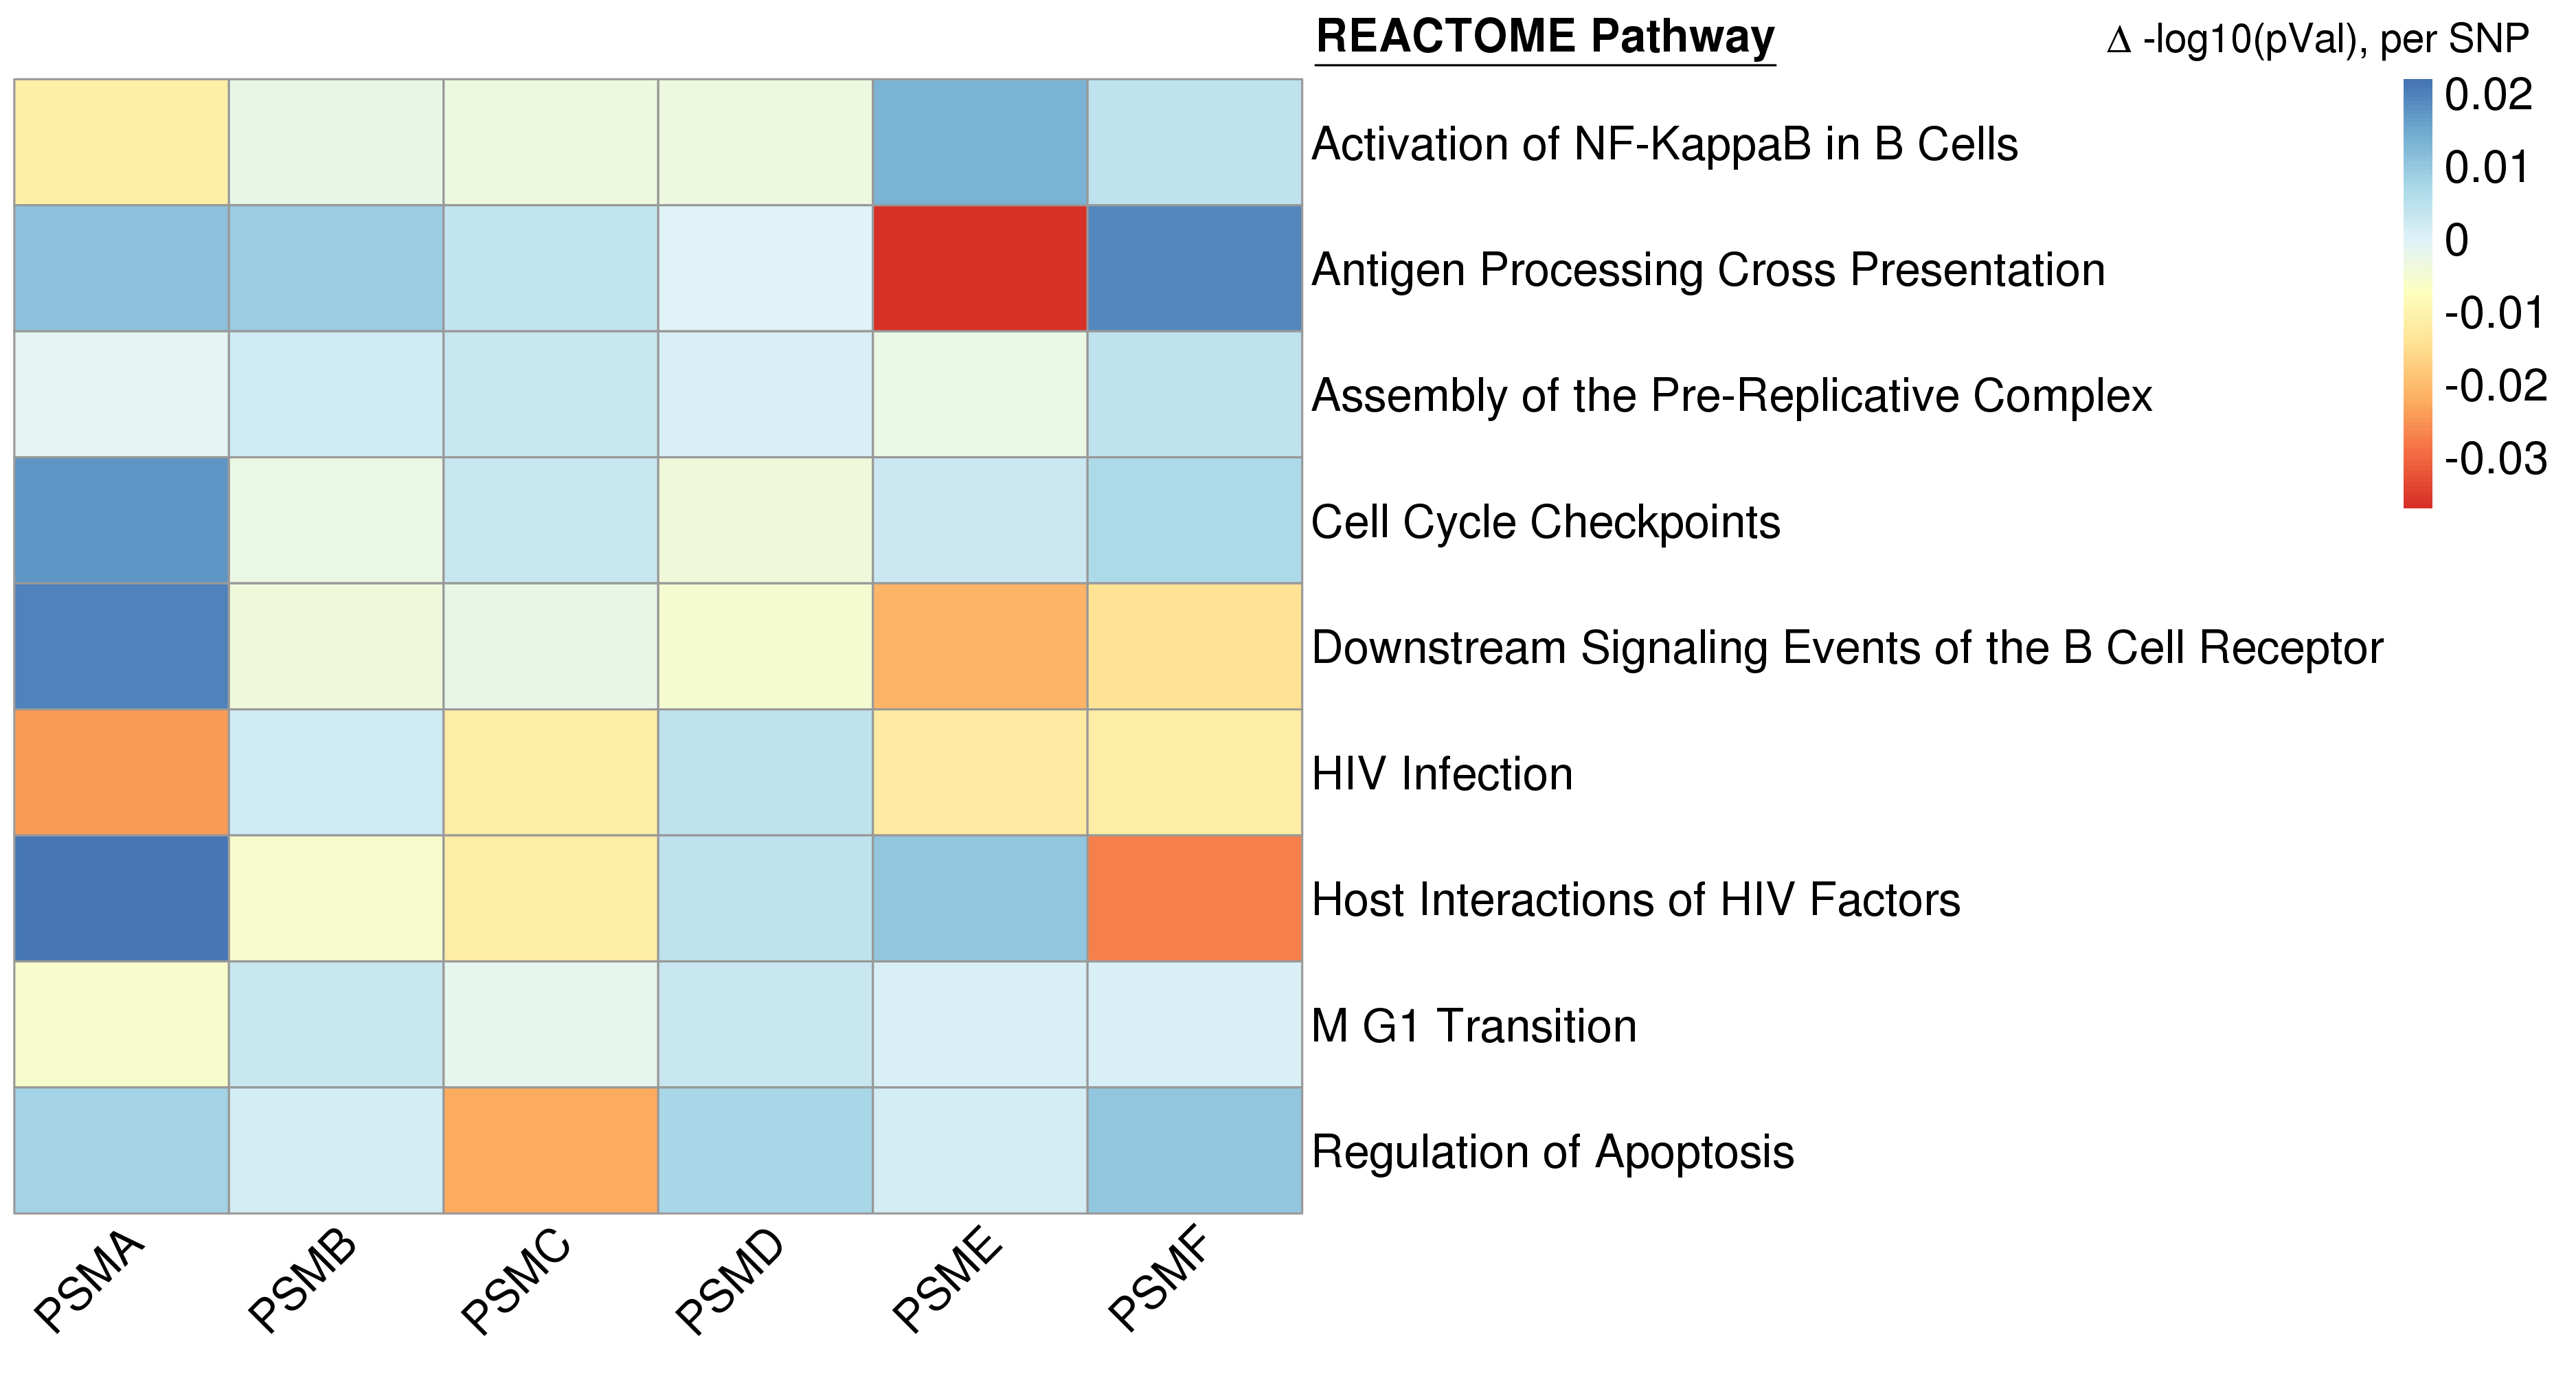
\includegraphics[scale=.5]{Images/Supp/InterPath_Supp_Figure_Proteaseome_Heatplots_Chinese_Loop_vs3.png}}
\par
\subfloat[]{\resizebox{1.1\columnwidth}{!}{
 \hspace*{-1.75cm}
 \begin{tabular}{cc|ccc}
  \hline
\textbf{Proteasome} & \textbf{SNPs} & \textbf{REACTOME} & \textbf{SNPs} & \textbf{MAPIT-R} \\
 \textbf{Gene Family} & & \textbf{Pathway} & & \textbf{$p$-Value} \\
  \hline
PSMA & 13 & Activation of NF-KappaB in B Cells & 433 & 5.27E-01  \\
PSMB & 74 & Antigen Processing Cross Presentation & 771 & 1.11E-02 \\
PSMC & 18 & Assembly of the Pre-Replicative Complex & 292 & 8.77E-01 \\
PSMD & 58 & Cell Cycle Checkpoints & 589 & 5.41E-01  \\
PSME & 12 & Downstream Signaling Events of the B Cell Receptor & 698 & 1.40E-01 \\
PSMF & 16 & HIV Infection & 1266 & 3.68E-03 \\
 & & Host Interactions of HIV Factors & 902 & 4.24E-02 \\
 & & M G1 Transition & 400 & 8.20E-01 \\
 & & Regulation of Apoptosis & 527 & 2.26E-02 \\
  \hline
\end{tabular}}}
\caption[TBD]{\textbf{Proteasome gene family leave-one-out MAPIT-R reruns, REACTOME-BMI-Chinese}. (a) The figure shows the change in original MAPIT-R -$\log_{10}$ $p$-value for each presented REACTOME pathway when each proteasome gene family is removed one at a time. The analyses were conducted in the BMI-Chinese subgroup combination. The $x$-axis shows each proteasome gene family and the $y$-axis shows each REACTOME pathway. Each column has been scaled by the number of SNPs present in the given gene family and, as a result, the heatplot specifically shows the -$\log_{10}$ $p$-value change per SNP. (b) The table shows the number of SNPs that are present in each proteasome gene family (left) and each REACTOME pathway (right). The original MAPIT-R $p$-values for each pathway are also shown (right).}
\label{InterPath-Supp-Figure-Prot-Heatplots-Chinese}
\end{figure}
\clearpage
\addtocounter{figure}{-1}
\addtocounter{CharNumber5}{1}

\begin{figure}[ht]
\centering
\vspace*{-.5cm}
\subfloat[]{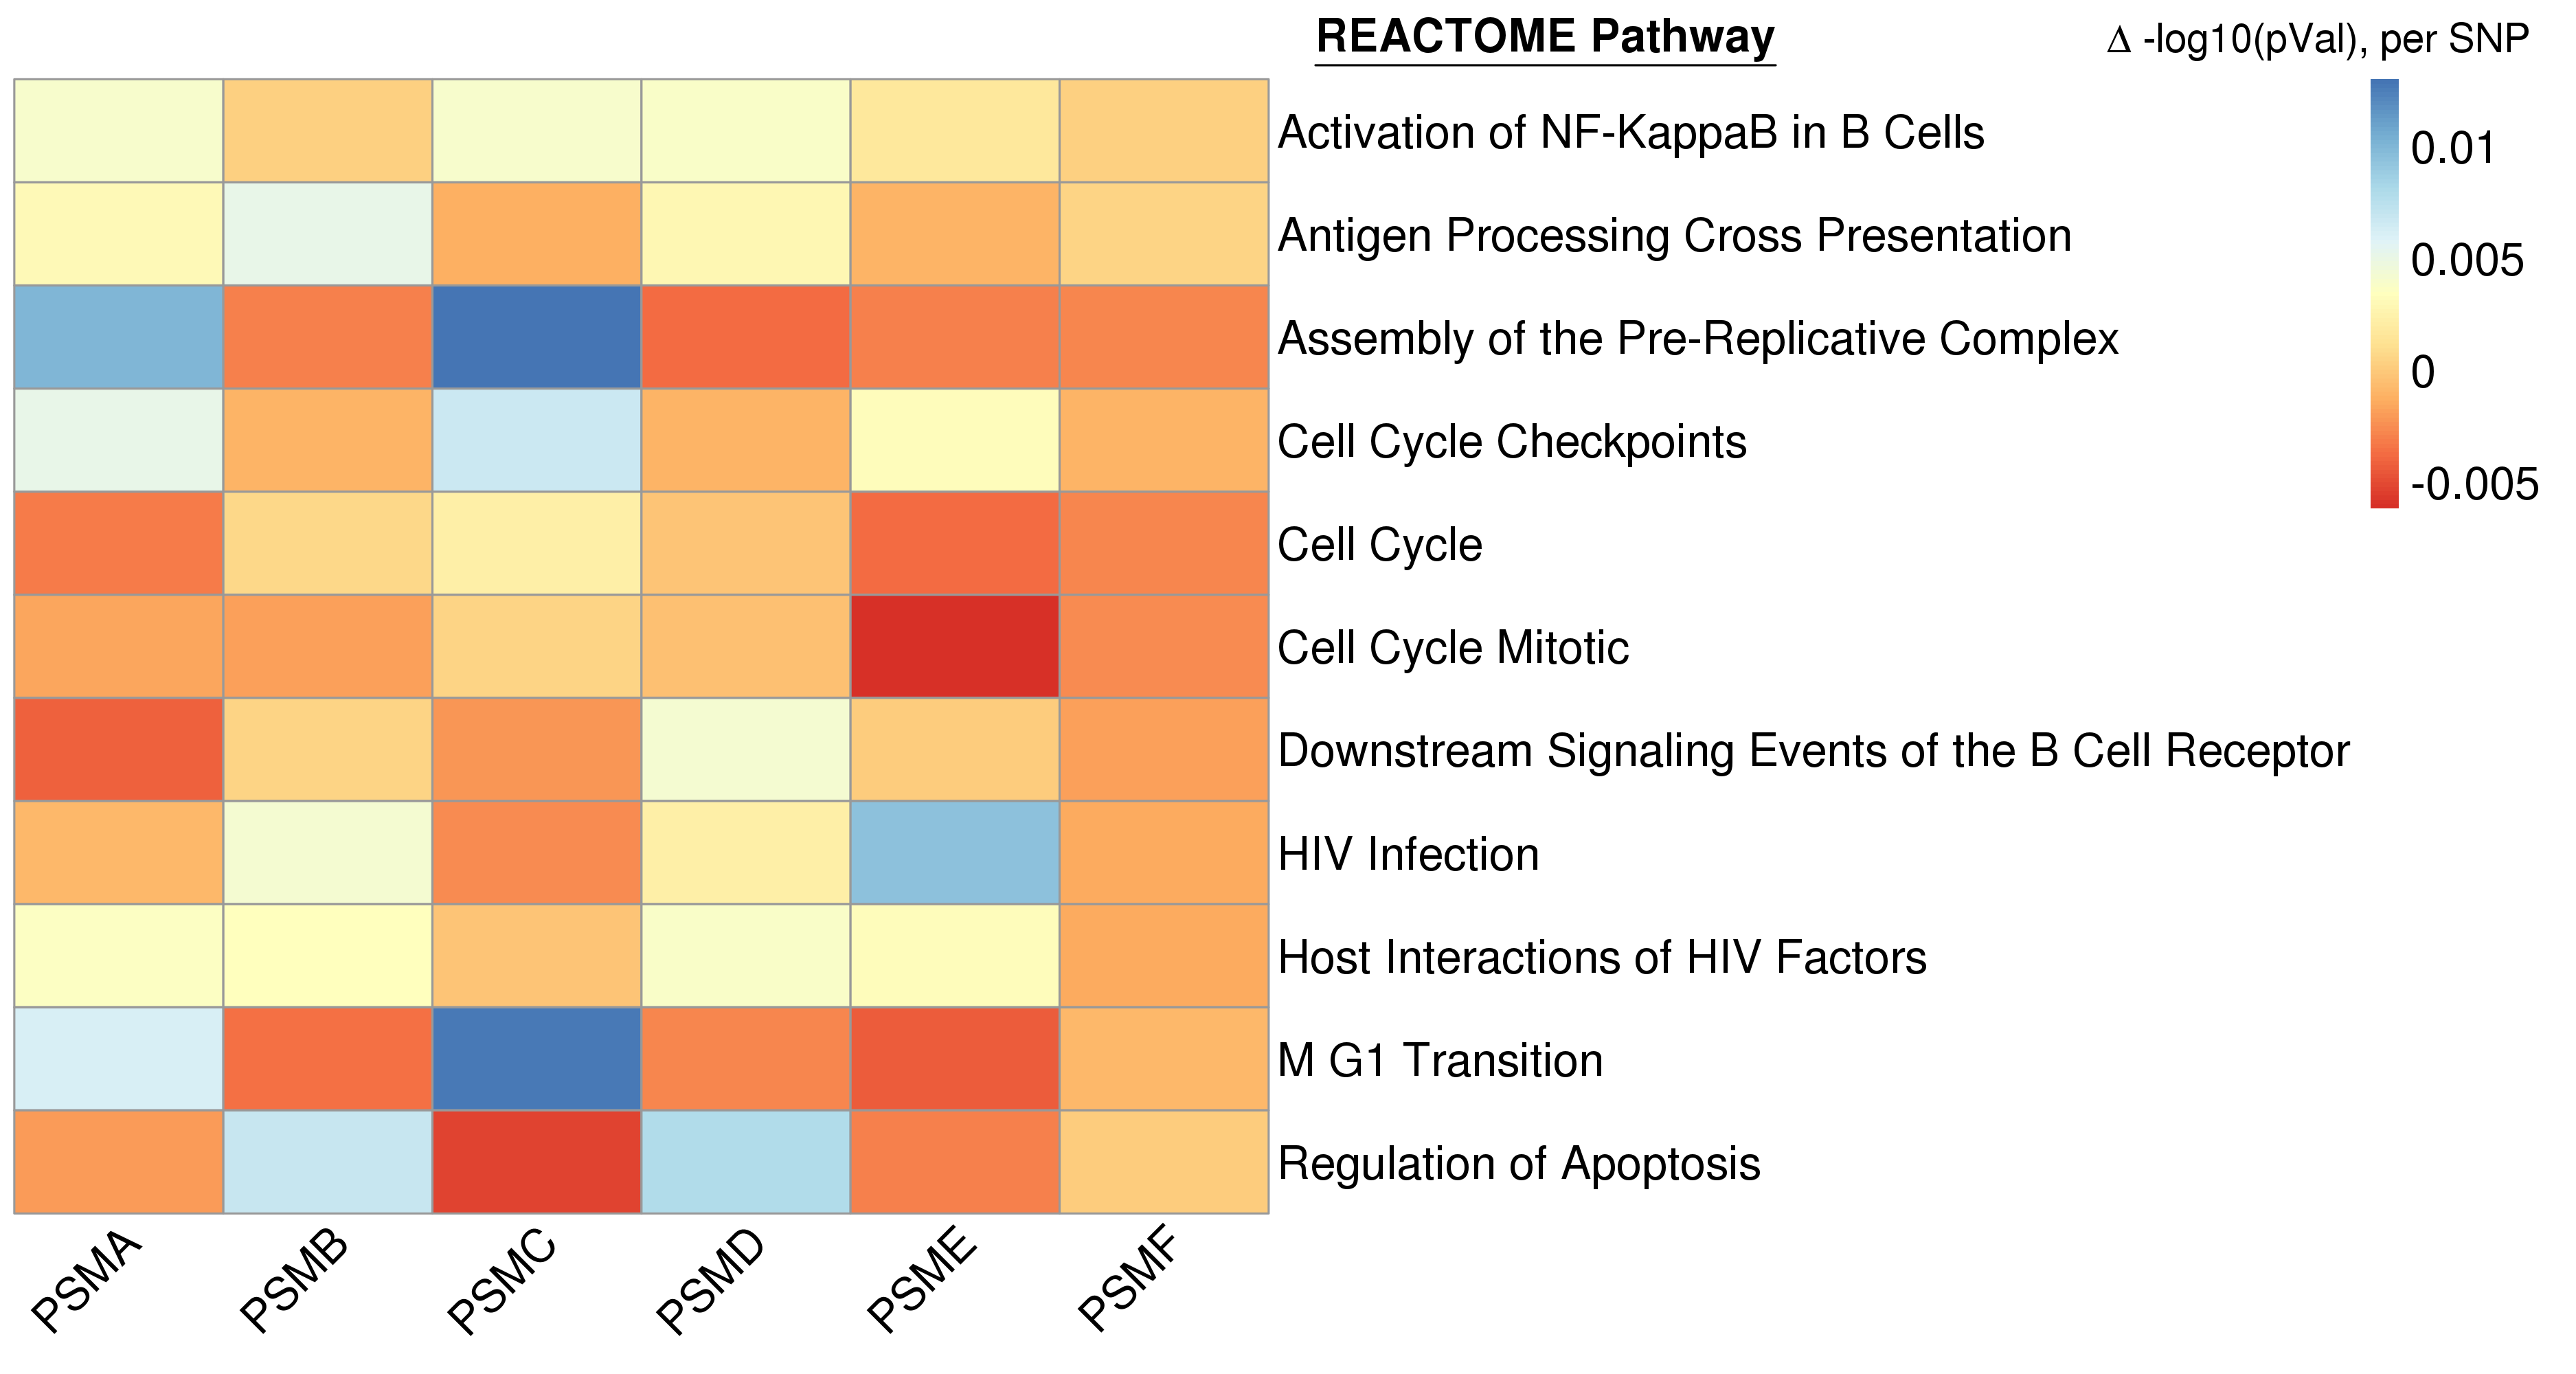
\includegraphics[scale=.5]{Images/Supp/InterPath_Supp_Figure_Proteaseome_Heatplots_Indian_Loop_vs3.png}}
\par
\subfloat[]{\resizebox{1.1\columnwidth}{!}{
 \hspace*{-1.75cm}
 \begin{tabular}{cc|ccc}
  \hline
\textbf{Proteasome} & \textbf{SNPs} & \textbf{REACTOME} & \textbf{SNPs} & \textbf{MAPIT-R} \\
 \textbf{Gene Family} & & \textbf{Pathway} & & \textbf{$p$-Value} \\
  \hline
PSMA & 29 & Activation of NF-KappaB in B Cells & 618 & 9.978E-01  \\
PSMB & 85 & Antigen Processing Cross Presentation & 977 & 4.476E-01 \\
PSMC & 25 & Assembly of the Pre-Replicative Complex & 427 & 5.019E-01 \\
PSMD & 78 & Cell Cycle Checkpoints & 909 & 8.042E-01 \\
PSME & 21 & Cell Cycle & 3361 & 1.873E-01 \\
PSMF & 21 & Cell Cycle Mitotic & 2656 & 2.316E-01 \\
 & & Downstream Signaling Events of the B Cell Receptor & 1037 & 5.534E-01 \\
 & & HIV Infection & 1836 & 9.803E-02 \\
 & & Host Interactions of HIV Factors & 1278 & 3.788E-01 \\
 & & M G1 Transition & 590 & 4.658E-01 \\
 & & Regulation of Apoptosis & 754 & 5.606E-01 \\
  \hline
\end{tabular}}}
\caption[TBD]{\textbf{Proteasome gene family leave-one-out MAPIT-R reruns, REACTOME-BMI-Indian}. (a) The figure shows the change in original MAPIT-R -$\log_{10}$ $p$-value for each presented REACTOME pathway when each proteasome gene family is removed one at a time. The analyses were conducted in the BMI-Indian subgroup combination. The $x$-axis shows each proteasome gene family and the $y$-axis shows each REACTOME pathway. Each column has been scaled by the number of SNPs present in the given gene family and, as a result, the heatplot specifically shows the -$\log_{10}$ $p$-value change per SNP. (b) The table shows the number of SNPs that are present in each proteasome gene family (left) and each REACTOME pathway (right). The original MAPIT-R $p$-values for each pathway are also shown (right).}
\label{InterPath-Supp-Figure-Prot-Heatplots-Indian}
\end{figure}
\clearpage
\addtocounter{figure}{-1}
\addtocounter{CharNumber5}{1}

\begin{figure}[ht]
\centering
\vspace*{-.5cm}
\subfloat[]{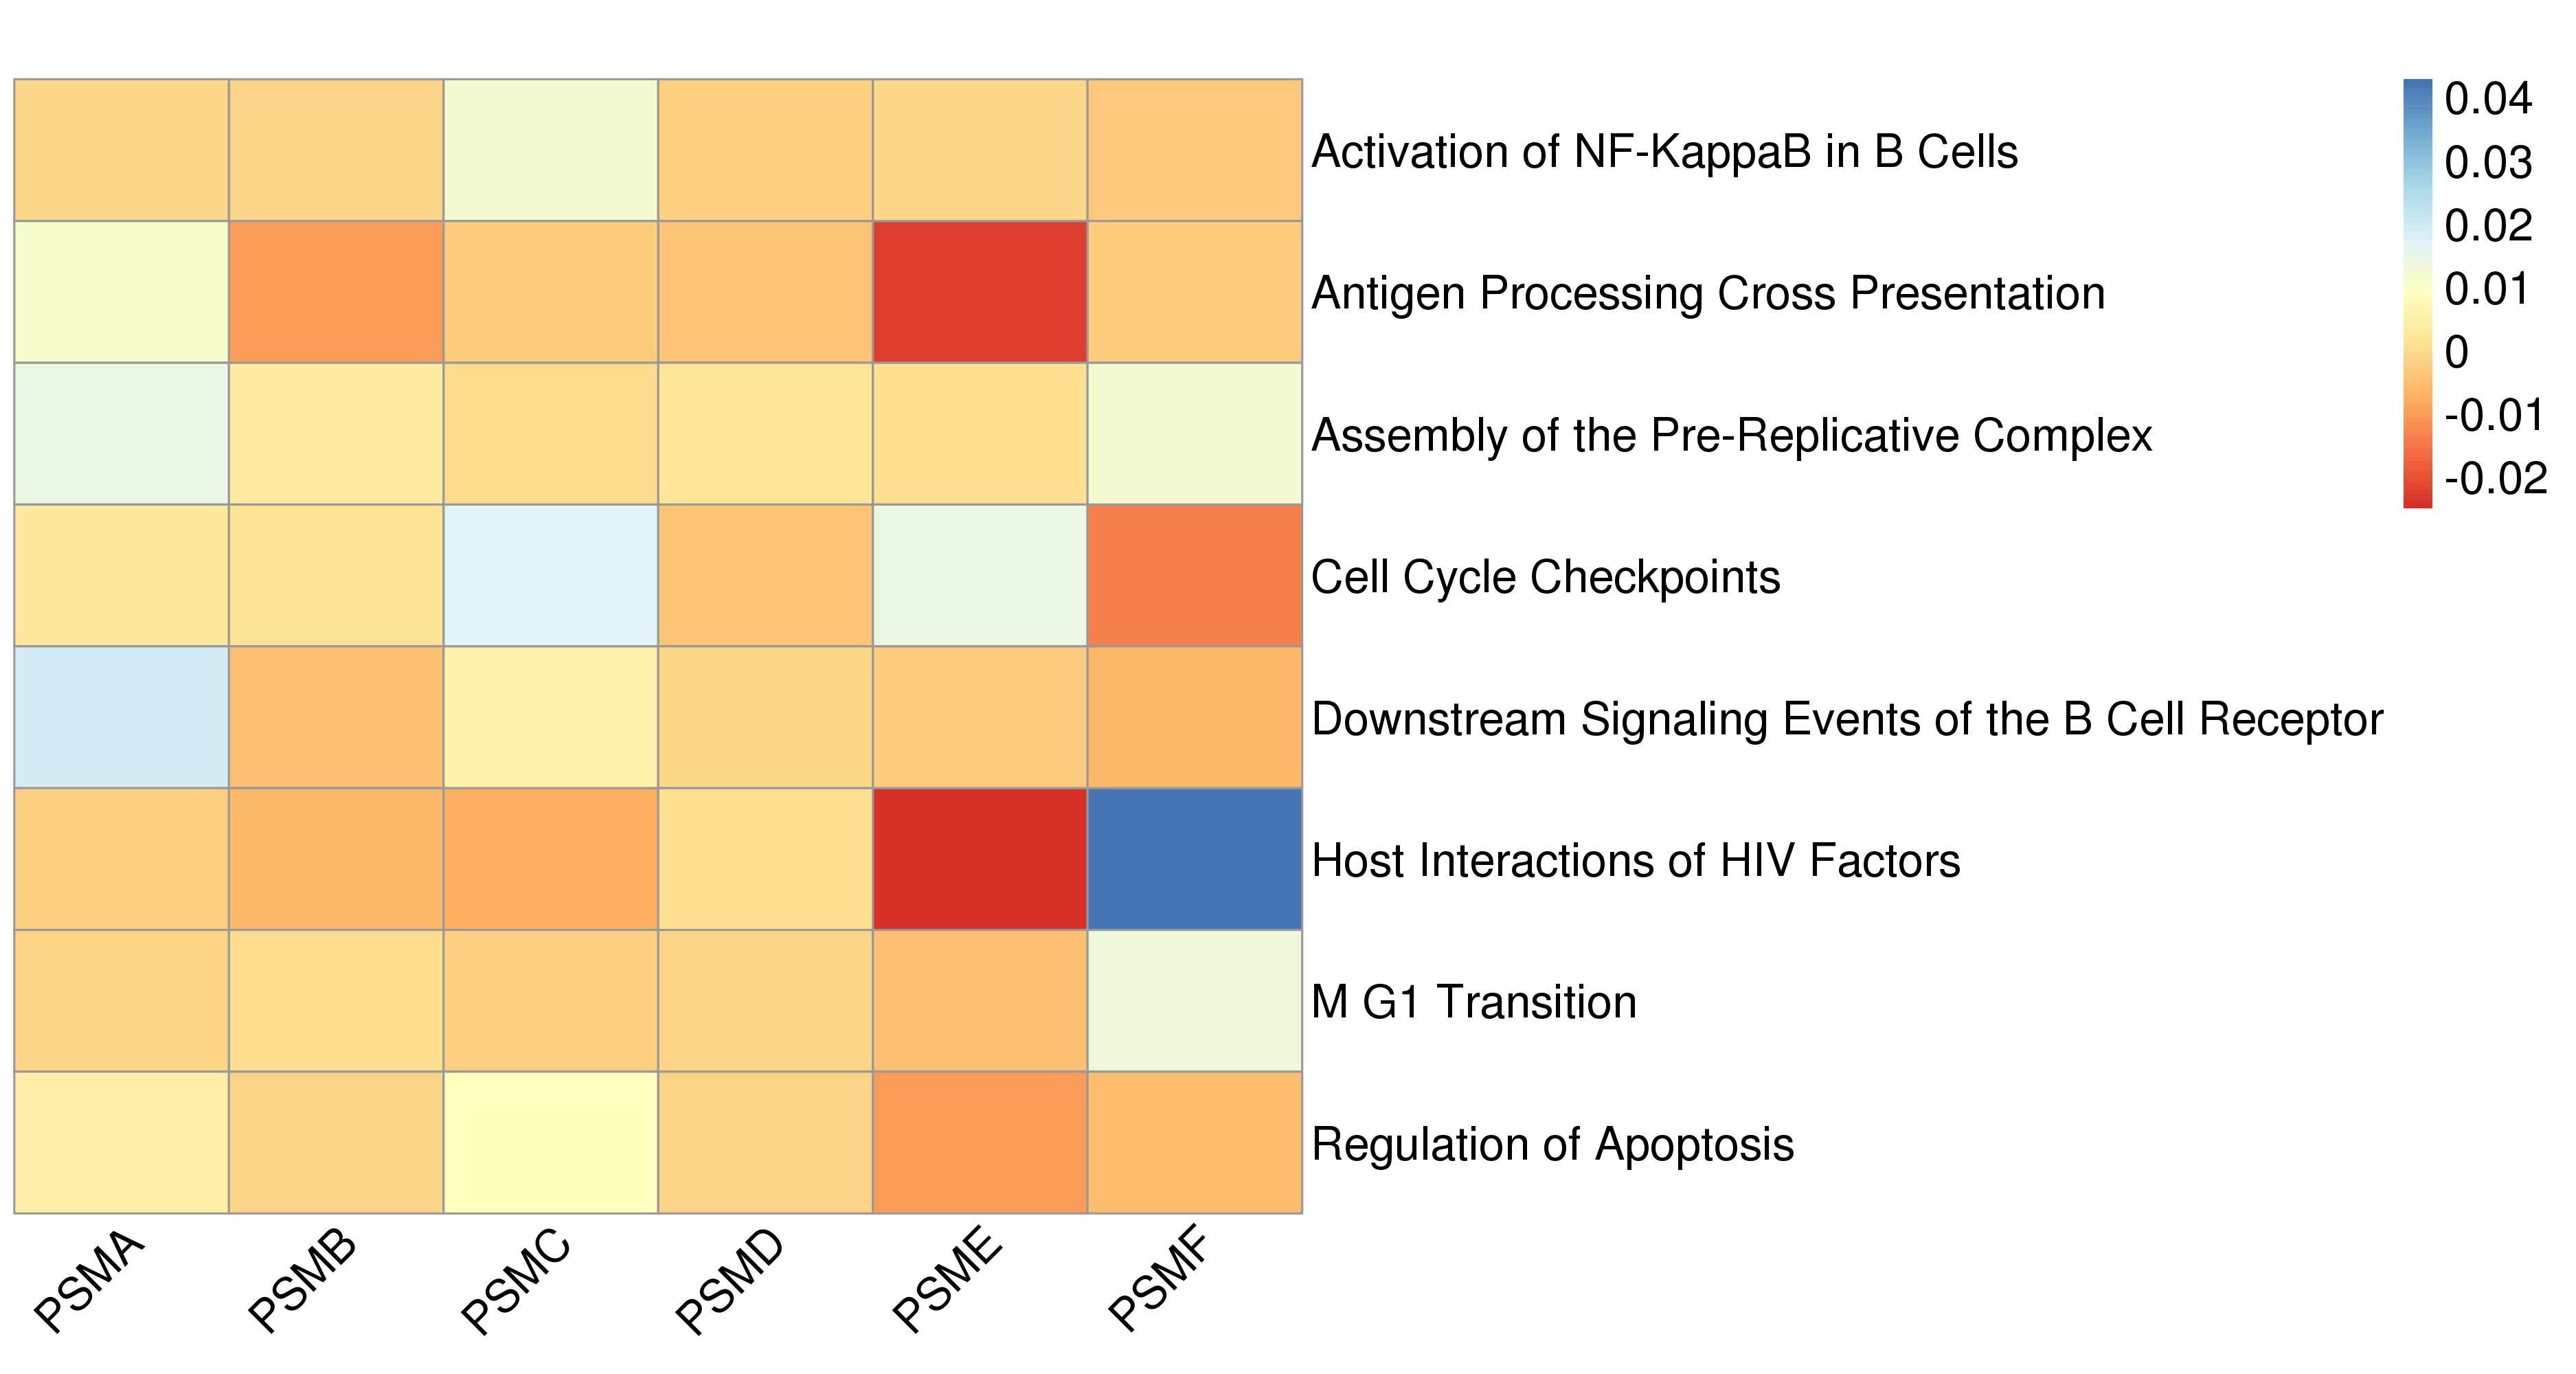
\includegraphics[scale=.5]{Images/Supp/InterPath_Supp_Figure_Proteaseome_Heatplots_Pakistani_Loop_vs3.png}}
\par
\subfloat[]{\resizebox{1.1\columnwidth}{!}{
 \hspace*{-1.75cm}
 \begin{tabular}{cc|ccc}
  \hline
\textbf{Proteasome} & \textbf{SNPs} & \textbf{REACTOME} & \textbf{SNPs} & \textbf{MAPIT-R} \\
 \textbf{Gene Family} & & \textbf{Pathway} & & \textbf{$p$-Value} \\
  \hline
PSMA & 30 & Activation of NF-KappaB in B Cells & 643 & 4.61E-01  \\
PSMB & 90 & Antigen Processing Cross Presentation & 1036 & 8.74E-03 \\
PSMC & 24 & Assembly of the Pre-Replicative Complex & 444 & 9.73E-01 \\
PSMD & 86 & Cell Cycle Checkpoints & 940 & 1.63E-01 \\
PSME & 21 & Downstream Signaling Events of the B Cell Receptor & 1073 & 6.57E-02 \\
PSMF & 22 & Host Interactions of HIV Factors & 1315 & 1.00E-01 \\
 & & M G1 Transition & 612 & 6.66E-01 \\
 & & Regulation of Apoptosis & 774 & 5.16E-02 \\
  \hline
\end{tabular}}}
\caption[TBD]{\textbf{Proteasome gene family leave-one-out MAPIT-R reruns, REACTOME-BMI-Pakistani}. (a) The figure shows the change in original MAPIT-R -$\log_{10}$ $p$-value for each presented REACTOME pathway when each proteasome gene family is removed one at a time. The analyses were conducted in the BMI-Pakistani subgroup combination. The $x$-axis shows each proteasome gene family and the $y$-axis shows each REACTOME pathway. Each column has been scaled by the number of SNPs present in the given gene family and, as a result, the heatplot specifically shows the -$\log_{10}$ $p$-value change per SNP. (b) The table shows the number of SNPs that are present in each proteasome gene family (left) and each REACTOME pathway (right). The original MAPIT-R $p$-values for each pathway are also shown (right).}
\label{InterPath-Supp-Figure-Prot-Heatplots-Pakistani}
\end{figure}
\clearpage
\addtocounter{figure}{-1}
\addtocounter{CharNumber5}{1}

\addtocounter{figure}{1}
\renewcommand{\thefigure}{\arabic{figure}}

\setlength{\footskip}{3cm}
\begin{figure}[htbp]
\centering
\vspace*{-2cm}
\includegraphics[scale=.2]{Images/Supp/InterPath_Supp_Figure_IBS_AllPops_vs4_noHLA.png}
\caption[TBD]{\textbf{Pathway-level genetic diversity vs. MAPIT-R results for all database-phenotype-subgroup combinations}. Caption continued on next page.}
\label{InterPath-Supp-Figure-IBS-AllPops}
\end{figure}
\clearpage
\setlength{\footskip}{1cm}
\addtocounter{figure}{-1}

\begin{figure} [t!]
\caption[TBD]{\textbf{Pathway-level genetic diversity vs. MAPIT-R results for all database-phenotype-subgroup combinations}. The figure shows the mean pairwise IBS proportions per pathway plotted against each pathway's MAPIT-R $p$-value for every pathway database-phenotype-UKB subgroup combination. IBS proportions were calculated per pathway by using that pathway's set of SNPs, were calculated pairwise between every set of individuals in the subgroup, and then averaged across each of these pairs for a final, single summary metric. We observe across the majority of combinations no significant relationship between mean pairwise IBS proportion and MAPIT-R $p$-value.}
\label{InterPath-Supp-Figure-IBS-AllPops-Caption}
\end{figure}
\clearpage

%\begin{figure}[htbp]
%\centering
%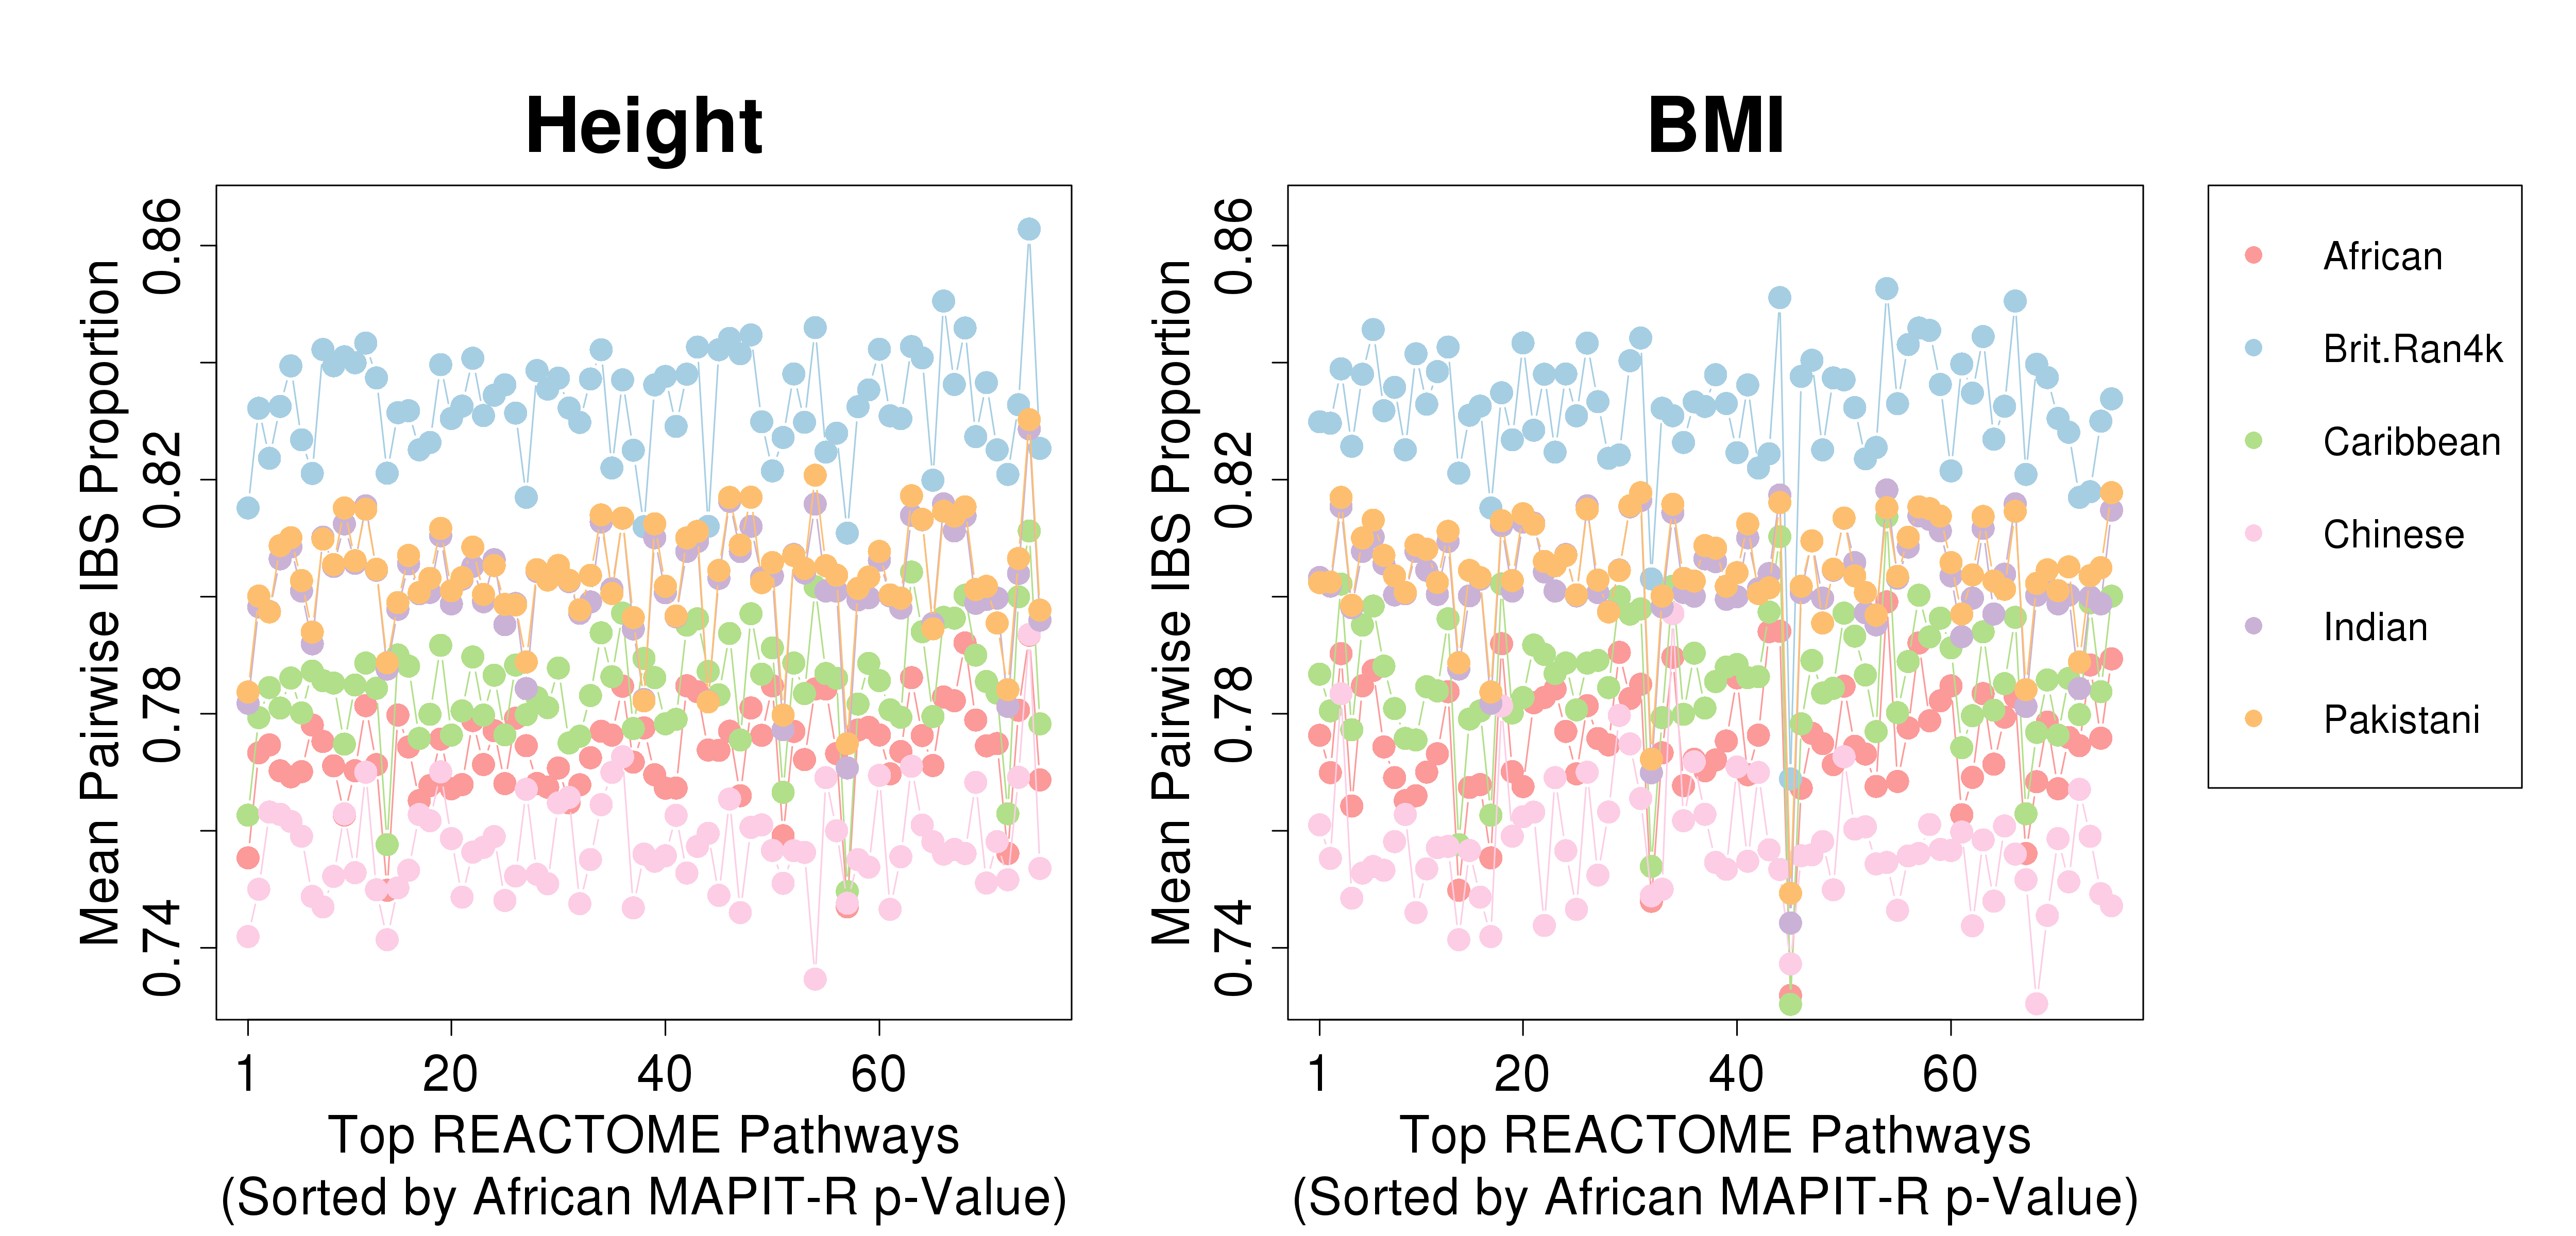
\includegraphics[scale=.35]{Images/Supp/InterPath_Supp_Figure_IBS_AllPopComps_vs3_REACTOME.png}
%\caption[TBD]{\textbf{Pathway-level genetic diversity across all UKB subgroups for top African MAPIT-R REACTOME pathways}. The figure plots the mean pairwise IBS proportions of each UKB subgroup for the top 75 REACTOME pathways (sorted by MAPIT-R African subgroup $p$-value) for each pathway database-phenotype combination. Most variation in mean pairwise IBS proportions varies moreso based on the pathways themselves and not on ancestry; subgroups differ between one another mostly at the same levels across each pathway.}
%\label{InterPath-Supp-Figure-IBS-AllPopComps-REACTOME}
%\end{figure}
%\clearpage

\begin{figure}[htbp]
\centering
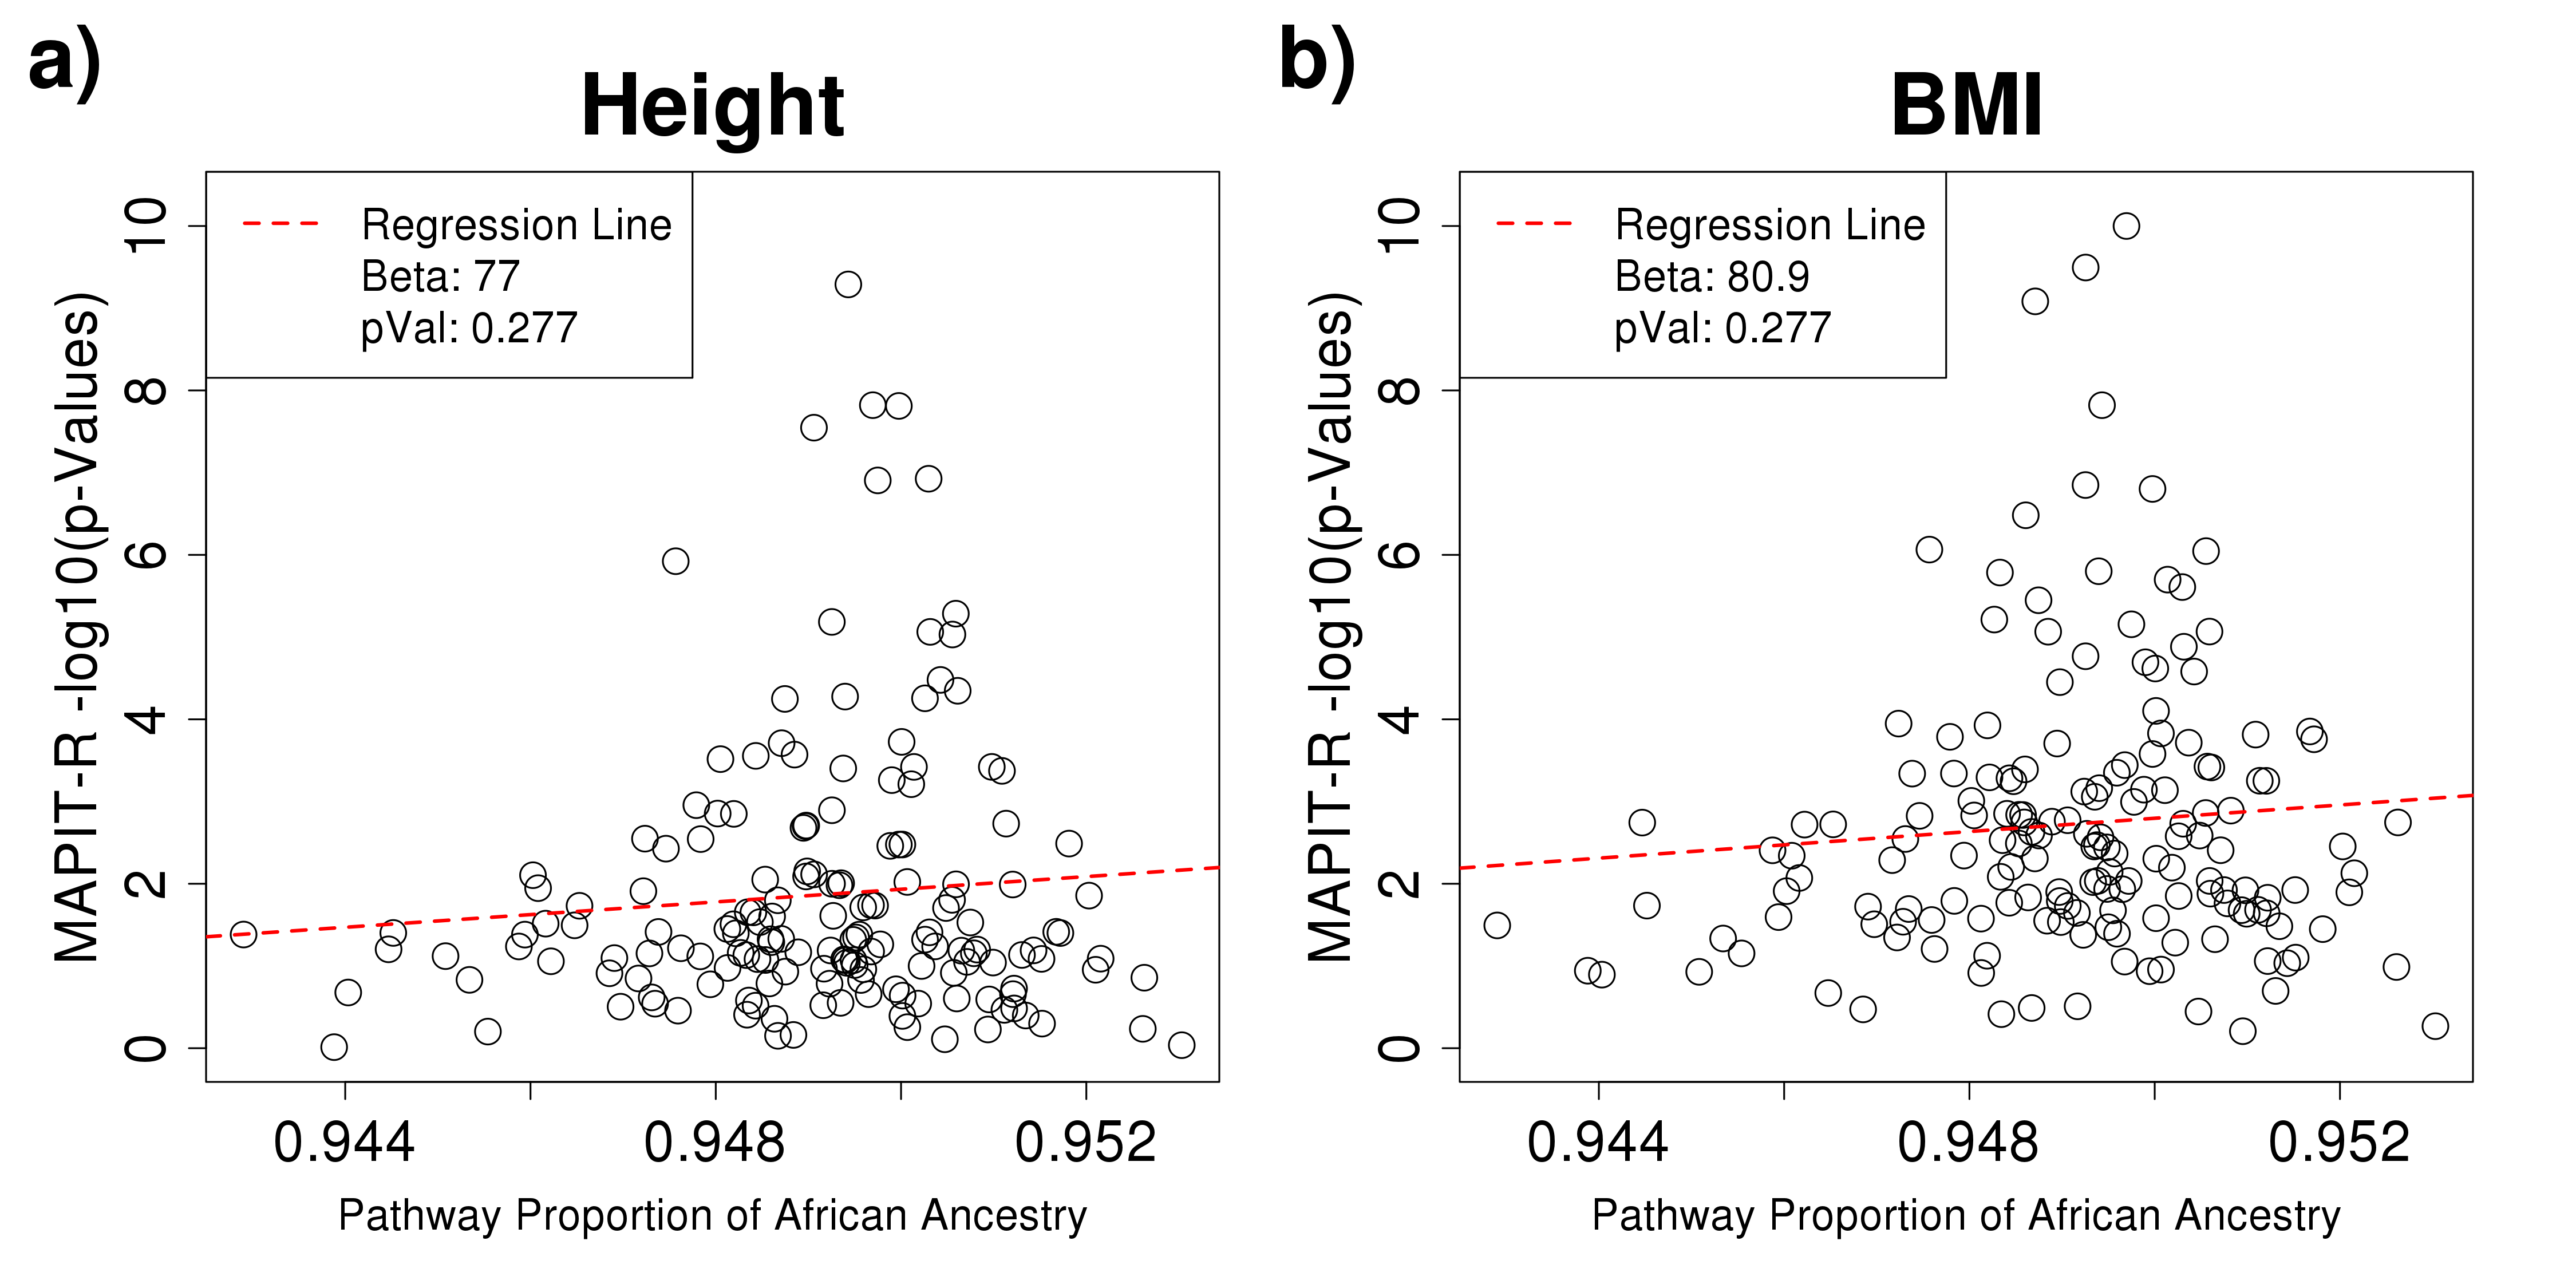
\includegraphics[scale=.35]{Images/Supp/InterPath_Supp_Figure_RFMix_vs2_African_KEGG_noHLA.png}
\caption[TBD]{\textbf{Pathway-level genetic diversity vs. MAPIT-R results in the African subgroup and KEGG database}. The figure shows the mean pairwise IBS proportions per pathway plotted against each pathway's MAPIT-R $p$-value for the African subgroup KEGG (a) height and (b) BMI analysis. IBS proportions were calculated per pathway by using each pathway's set of SNPs to derive pairwise IBS values between every set of individuals in the subgroup, and then averaging across each of these pairs for a final summary metric. Results with REACTOME database pathways can be found in Supplementary Figure \ref{InterPath-Main-Figure-RFMix-African-REACTOME}. We observe across the majority of our combinations no significant relationship between a pathway's mean pairwise IBS proportion and its MAPIT-R $p$-value.}
\label{InterPath-Supp-Figure-RFMix-African-KEGG}
\end{figure}
\clearpage

\setlength{\footskip}{3cm}
\begin{figure}[htbp]
\centering
\vspace*{-2cm}
\includegraphics[scale=.2]{Images/Supp/InterPath_Supp_Figure_PC1Loading_AllPaths_vs2_noHLA.png}
\caption[TBD]{\textbf{Relationship between MAPIT-R $p$-values and proportions of pathway SNPs loaded on PC1, all pathways}. Caption continued on next page.}
\label{InterPath-Supp-Figure-PC1Loading-AllPaths}
\end{figure}
\clearpage
\setlength{\footskip}{1cm}

\addtocounter{figure}{-1}
\begin{figure} [t!]
  \caption{\textbf{Relationship between MAPIT-R $p$-values and proportions of pathway SNPs loaded on PC1, all pathways}. The figure shows the proportion of SNPs within a given pathway that are strongly loaded on local PC1 plotted against that pathway's MAPIT-R -$\log_{10}$ $p$-value. All pathway sizes were used for this analysis. `Local' here refers to PCA having been conducted within-subgroup. SNPs are designated as `strongly loaded' on local PC1 if they are within the 10\% tails of the loading SNP score distributions. We observe that there is no significantly positive relationship between MAPIT-R $p$-values and proportion of SNPs that are strongly loaded on PC1 for any pathway database-phenotype-subgroup combination.}
\label{InterPath-Supp-Figure-PC1Loading-AllPaths-Caption}
\end{figure}
\clearpage

\setlength{\footskip}{2cm}
\begin{figure}[htbp]
\centering
\vspace*{-1.75cm}
\hspace*{-1cm}
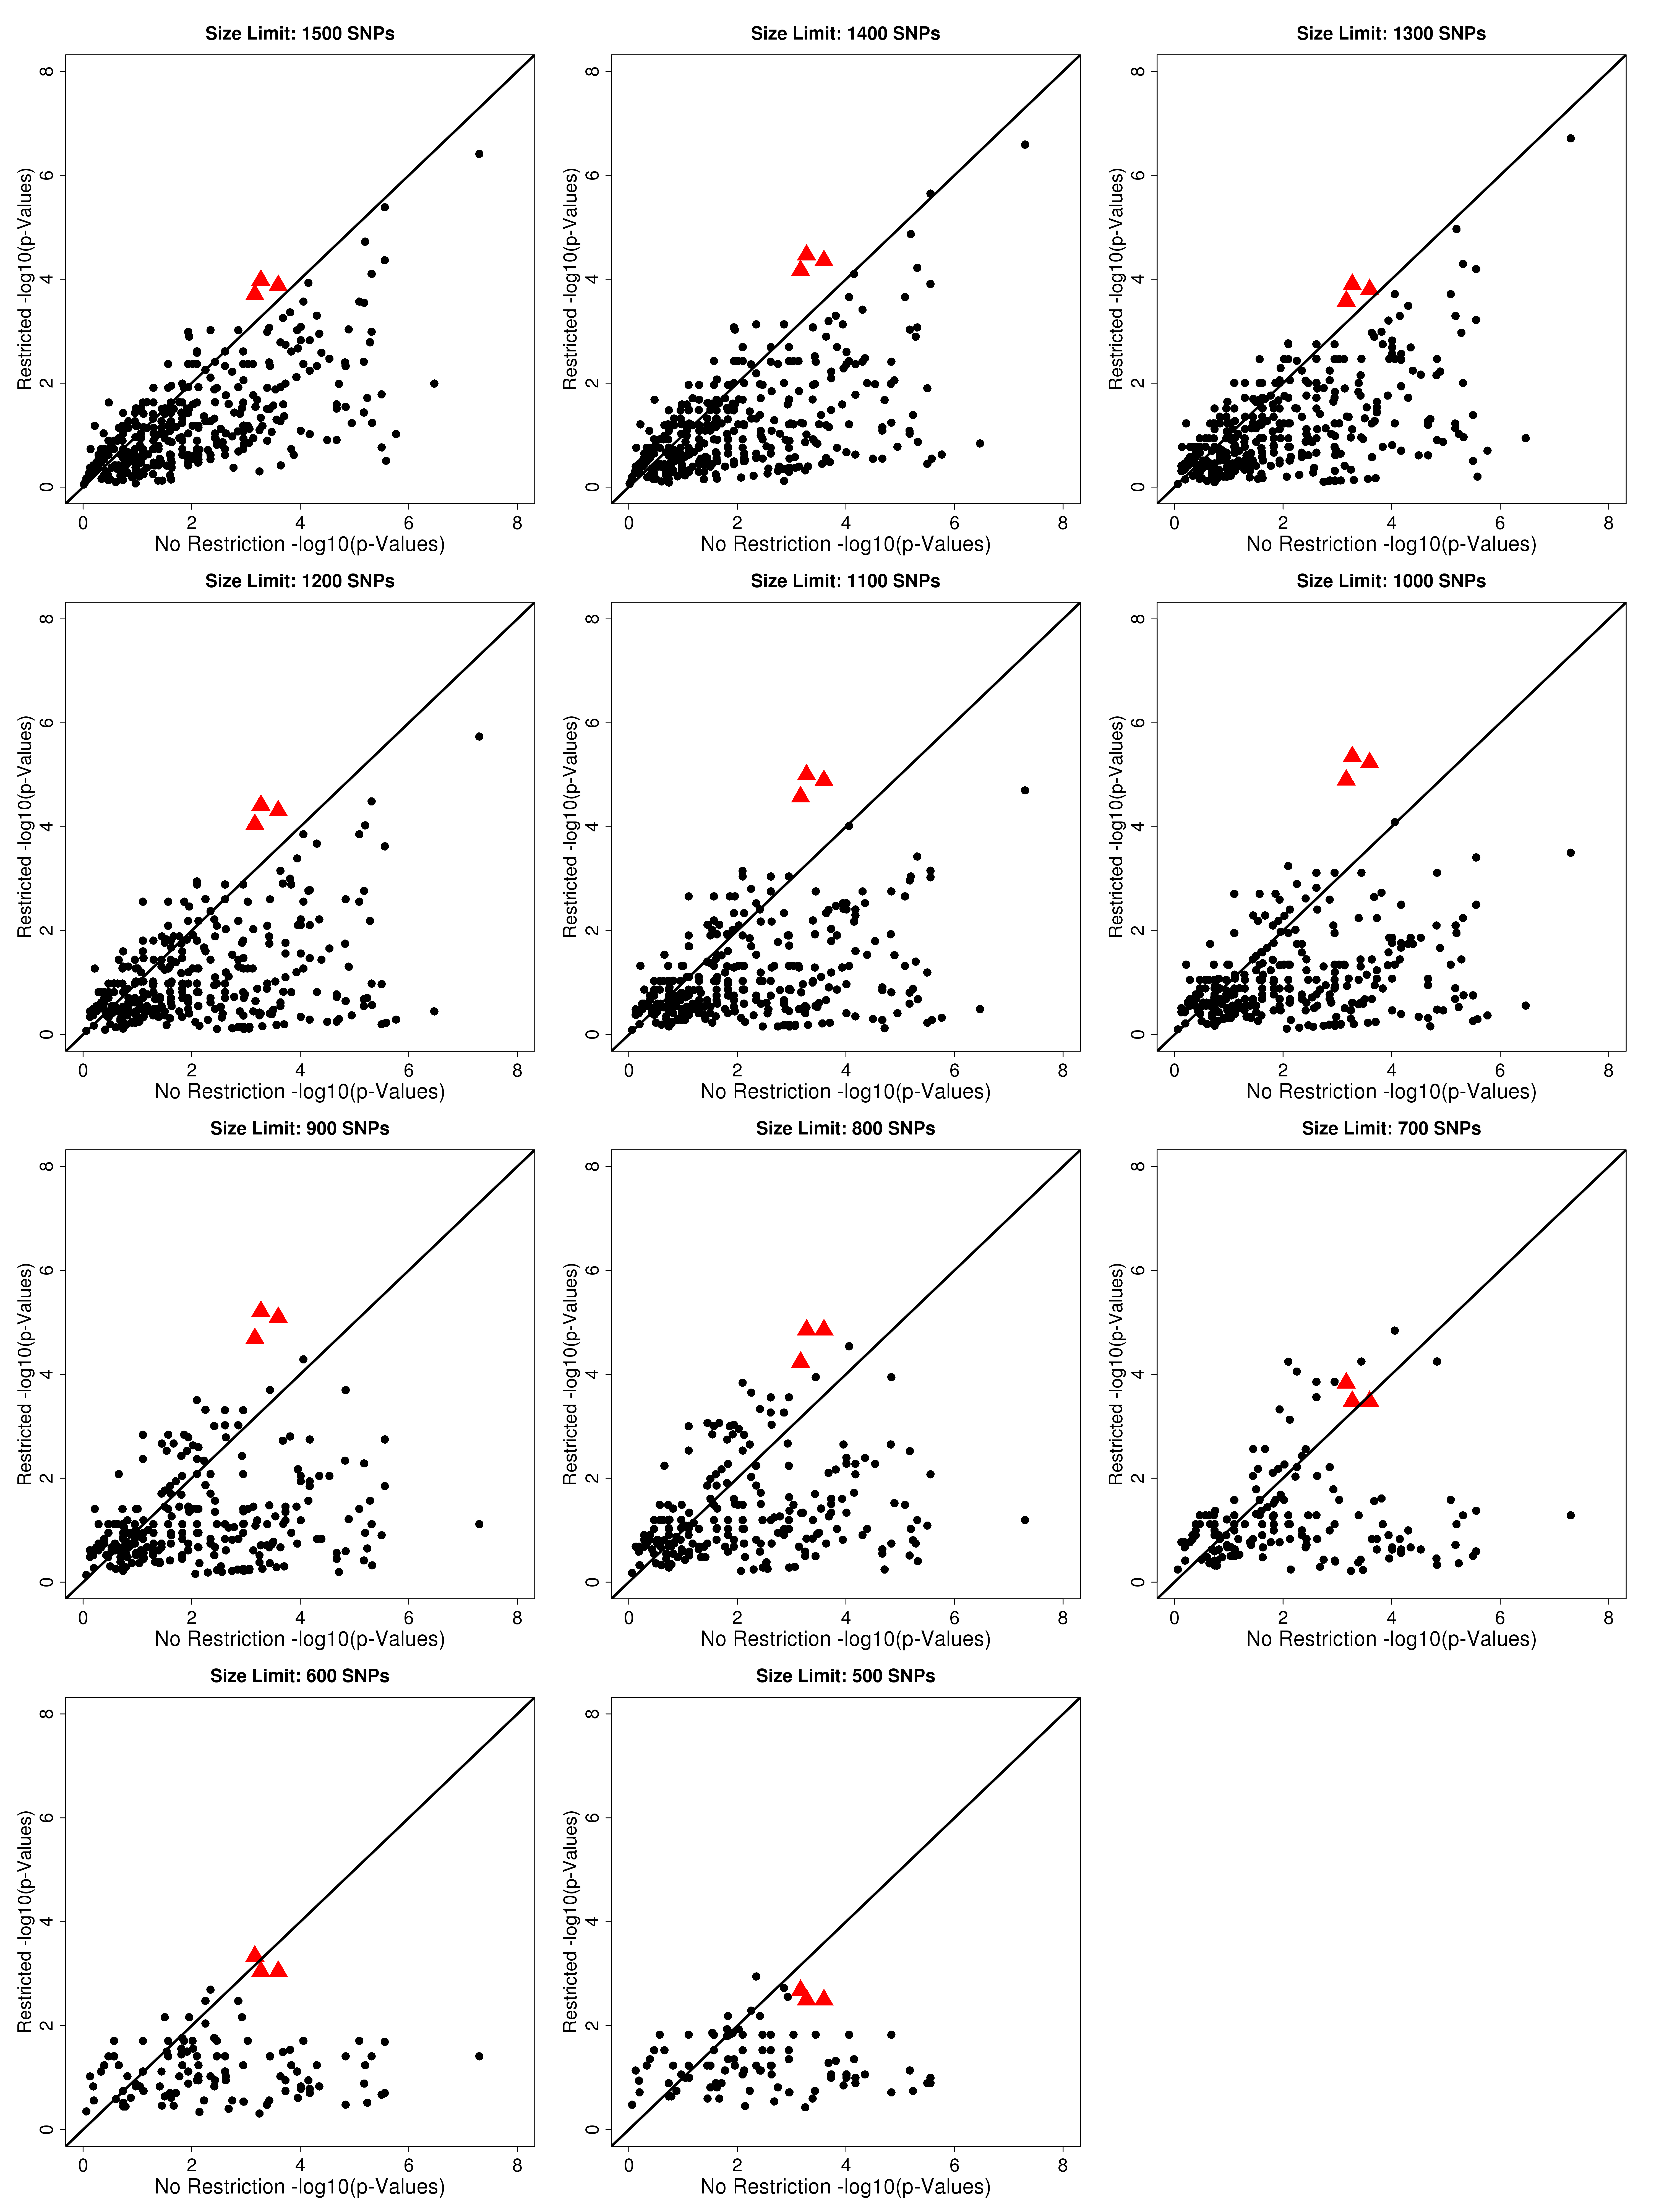
\includegraphics[scale=.325]{Images/Supp/InterPath_Supp_Figure_Hypergemeotric_SizeThresholds_vs1.png}
\caption[TBD]{\textbf{Impact of pathway size thresholds on hypergeometric enrichment analyses}. Caption continued on next page.}
\label{InterPath-Supp-Figure-Hypergeoemtric-SizeThresholds}
\end{figure}
\clearpage
\setlength{\footskip}{1cm}

\addtocounter{figure}{-1}
\begin{figure} [t!]
  \caption{\textbf{Impact of pathway size thresholds on hypergeometric enrichment analyses}. The figure shows multiple comparisons of size-restricted hypergeometric enrichment analyses versus unrestricted hypergeometric enrichment analyses using incrementally decreasing pathway size thresholds. Size thresholds change from 1,500 SNPs to 500 SNPs in 100 SNP increments. In each plot the $x$-axis is the unrestricted hypergeometric $p$-value for each gene and the $y$-axis is the size-restricted hypergeometric $p$-value for each gene. Red triangles represent results for each gene belonging to a proteasome gene family ({\emph{PSMA}}, {\emph{PSMB}}, {\emph{PSMC}}, {\emph{PSMD}}, {\emph{PSME}}, and {\emph{PSMF}}). Note that there are only three triangles since most proteasome genes are assigned to the same pathways.}
\label{InterPath-Supp-Figure-Hypergeoemtric-SizeThresholds-Caption}
\end{figure}
\clearpage

\section{Supplementary Tables}\label{Supplementary-Tables}

\begin{table}[ht]
\centering
\begin{tabular}{ccccc}
  \hline
\textbf{UK BioBank} & \textbf{Individuals} & \textbf{SNPs} & \textbf{KEGG} & \textbf{REACTOME} \\
\textbf{subgroup} & & & \textbf{Pathways} & \textbf{Pathways}  \\
  \hline
\textbf{Original subgroups:} & & & & \\
African & 3111 & 374466 & 180 & 658 \\ 
British.Ran4000 & 3848 & 600006 & 173 & 650 \\ 
Caribbean & 3833 & 410017 & 181 & 661 \\ 
Chinese & 1448 & 345221 & 153 & 626 \\ 
Indian & 5077 & 505854 & 181 & 662 \\ 
Pakistani & 1581 & 516806 & 141 & 596 \\ 
\\
\textbf{British Replicates:} & & & & \\
British.Ran4000.2 & 3869 & 599381 & 173 & 650 \\ 
British.Ran4000.3 & 3836 & 600654 & 173 & 649 \\ 
British.Ran4000.4 & 3838 & 599829 & 173 & 650 \\ 
British.Ran4000.5 & 3853 & 599442 & 173 & 650 \\ 
British.Ran10000 & 9603 & 597298 & 186 & 669 \\ 
British.Ran10000.2 & 9628 & 597577 & 186 & 669 \\ 
British.Ran10000.3 & 9636 & 597486 & 186 & 669 \\ 
British.Ran10000.4 & 9593 & 597369 & 186 & 669 \\ 
British.Ran10000.5 & 9596 & 597507 & 186 & 669 \\ 
  \hline
\end{tabular}
\caption[TBD]{\textbf{Pathways and subgroups of the UK BioBank analyzed in this study}. The table shows the individual, SNP, and pathway counts for each of the UKB subgroups analyzed in this study. `Original subgroups' refers to the multiple global human ancestries that were initially analyzed at the beginning of this study, and `British Replicates' refers specifically to the subgroups that were created to analyze multiple, independent random subsamples of the UKB British cohort. The number of individuals and SNPs post quality-control are shown in the second and third columns (see Materials and Methods), and the number of KEGG and REACTOME pathways analyzed in each subgroup are shown in the fourth and fifth columns. Note that for the `British Replicates' subgroups each group began with an independent set of either 4,000 or 10,000 individuals from the original UKB phenotype file.}
\label{InterPath-Supp-Table-UKBPopStats}
\end{table}
\clearpage

%Irish & 11575 & 588324 & 186 & 671 \\ 

%\textbf{Supplementary Tables 2a-d.} \textbf{Lists of New \bmass{} Multivariate Associations, per Dataset}. \\ Attached Excel sheets list new \bmass{} associations for each dataset analyzed.
%\bigskip \bigskip

\begin{table} [t!]
  \caption{\textbf{Lists of genome-wide significant MAPIT-R pathways, per subgroup}.  Attached Excel sheets list the pathways that were found to be MAPIT-R genome-wide significant in each UKB subgroup for the following phenotype and pathway database combinations: (a) KEGG+Height, (b) KEGG+BMI, (c) REACTOME+Height, and (d) REACTOME+BMI. Genome-wide significance was determined by using a Bonferroni-corrected $p$-value threshold of .05 divided by the number of pathways tested (Supplementary Table \ref{InterPath-Supp-Table-UKBPopStats}).}
\label{InterPath-Supp-Table-TopPathways-AllPaths-AllPhenos}
\end{table}
\clearpage

\setlength{\footskip}{4cm}
\begin{landscape}
\begin{table}[ht]
\vspace*{-1.5cm}
\centering
\hspace*{-3.5cm}
\begin{tabular}{ccccccccc}
  \hline
\textbf{Population} & \textbf{Pathway} & \textbf{Bonferroni} & \textbf{Bonferroni} & \textbf{Bonferroni} & \multicolumn{2}{c}{\textbf{.001 Threshold}} & \multicolumn{2}{c}{\textbf{.01 Threshold}} \\
\cline{6-7}
\cline{8-9}
 & \textbf{Counts} & \textbf{Threshold} & \textbf{Counts} & \textbf{FDR} & \textbf{Counts} & \textbf{FDR} & \textbf{Counts} & \textbf{FDR} \\ 
  \hline
\textbf{KEGG Height:} & & & & & & & \\
African & 1800 & 2.778E-04 & 0 & 0.000  & 1 & 0.056 & 10 & 0.556 \\ 
  British.Ran4000 & 1730 & 2.890E-04 & 0 & 0.000 & 0 & 0.000 & 13 & 0.751 \\ 
  Caribbean & 1810 & 2.762E-04 & 1 & 0.055 & 1 & 0.055 & 5 & 0.276 \\ 
  Chinese & 1530 & 3.268E-04 & 0 & 0.000 & 3 & 0.196 & 24 & 1.569 \\ 
  Indian & 1810 & 2.762E-04 & 1 & 0.055 & 1 & 0.055 & 20 & 1.105 \\ 
  Pakistani & 1410 & 3.546E-04 & 0 & 0.000 & 2 & 0.142 & 17 & 1.206 \\ 
  \\
  \textbf{KEGG BMI:} & & & & & & & \\
African & 1800 & 2.778E-04 & 0 & 0.000 & 1 & 0.056 & 10 & 0.556 \\ 
  British.Ran4000 & 1730 & 2.890E-04 & 0 & 0.000 & 0 & 0.000 & 13 & 0.751 \\ 
  Caribbean & 1810 & 2.762E-04 & 1 & 0.055 & 1 & 0.055 & 5 & 0.276 \\ 
  Chinese & 1530 & 3.268E-04 & 0 & 0.000 & 3 & 0.196 & 24 & 1.569 \\ 
  Indian & 1810 & 2.762E-04 & 1 & 0.055 & 1 & 0.055 & 20 & 1.105 \\ 
  Pakistani & 1410 & 3.546E-04 & 0 & 0.000 & 2 & 0.142 & 17 & 1.206 \\ 
  \\
  \textbf{REACTOME Height:} & & & & & & & \\
  African & 1800 & 2.778E-04 & 0 & 0.000 & 1 & 0.056 & 16 & 0.889 \\
  British.Ran4000 & 1730 & 2.890E-04 & 1 & 0.058 & 2 & 0.116 & 14 & 0.809 \\
  Caribbean & 1810 & 2.762E-04 & 0 & 0.000 & 1 & 0.055 & 25 & 1.381 \\
  Chinese & 1530 & 3.268E-04 & 0 & 0.000 & 1 & 0.065 & 24 & 1.569 \\
  Indian & 1810 & 2.762E-04 & 1 & 0.055 & 2 & 0.110 & 20 & 1.105 \\
  Pakistani & 1410 & 3.546E-04 & 0 & 0.000 & 2 & 0.142 & 15 & 1.064 \\
  \\
  \textbf{REACTOME BMI:} & & & & & & & \\
African & 6580 & 7.599E-05 & 1 & 0.015 & 4 & 0.061 & 39 & 0.593 \\
  British.Ran4000 & 6490 & 7.704E-05 & 1 & 0.015 & 4 & 0.062 & 52 & 0.801 \\
  Caribbean & 6610 & 7.564E-05 & 0 & 0.000 & 13 & 0.197 & 97 & 1.467 \\
  Chinese & 6260 & 7.987E-05 & 0 & 0.000 & 6 & 0.096 & 49 & 0.783 \\
  Indian & 6620 & 7.553E-05 & 0 & 0.000 & 3 & 0.045 & 66 & 0.997 \\
  Pakistani & 5960 & 8.389E-05 & 0 & 0.000 & 4 & 0.067 & 45 & 0.755 \\
   \hline
\end{tabular}
\caption[TBD]{\textbf{MAPIT-R false discovery rates at different significance thresholds, per subgroup}. Caption continued on next page. }
\label{InterPath-Supp-Table-AllPops-FDRs}
\end{table}
\end{landscape}
\clearpage
\setlength{\footskip}{1cm}

\addtocounter{table}{-1}
\begin{table} [t!]
  \caption{\textbf{MAPIT-R false discovery rates at different significance thresholds, per subgroup}. The table shows for various significance thresholds the false discovery rates observed from MAPIT-R when run on ten rounds of phenotype permutations for each UKB subgroup and pathway database. The first column lists the pathway database-phenotype-UKB subgroup combinations. The second column lists the total number of pathways that were tested across each of the ten phenotype permutations. The third column shows the $p$-value threshold associated with using the Bonferroni method of correction, also known as the `genome-wide significant' threshold. The fourth column shows the number of pathways across all ten phenotype permutation rounds that crossed this Bonferroni threshold. The fifth column shows the associated FDR associated with the fourth column. And the remaining six columns show the same setup as columns three to five but with a $p$-value threshold of either 0.001 or 0.01.}
\label{InterPath-Supp-Table-AllPops-FDRs-Caption}
\end{table}
\clearpage

\setlength{\footskip}{2cm}
\begin{landscape}
\begin{table}[ht]
\centering
\begin{tabular}{ll}
  \hline
 \textbf{Population} & \textbf{Pathways}\\
 \textbf{Comparison} & \\
  \hline
\textbf{African Vs.} & \\
\textbf{Caribbean:} & \\
 & KEGG\_ARRHYTHMOGENIC\_RIGHT\_VENTRICULAR\_CARDIOMYOPATHY\_ARVC \\
 & KEGG\_AXON\_GUIDANCE \\
 & KEGG\_CHEMOKINE\_SIGNALING\_PATHWAY \\
 & KEGG\_HYPERTROPHIC\_CARDIOMYOPATHY\_HCM \\
 & KEGG\_NATURAL\_KILLER\_CELL\_MEDIATED\_CYTOTOXICITY \\
 & KEGG\_VASCULAR\_SMOOTH\_MUSCLE\_CONTRACTION \\
\\
\textbf{African Vs.} & \\
\textbf{Chinese:} & \\
 & KEGG\_ALLOGRAFT\_REJECTION \\
 & KEGG\_ANTIGEN\_PROCESSING\_AND\_PRESENTATION \\
 & KEGG\_GRAFT\_VERSUS\_HOST\_DISEASE \\
 & KEGG\_SYSTEMIC\_LUPUS\_ERYTHEMATOSUS \\
 & KEGG\_TYPE\_I\_DIABETES\_MELLITUS \\
   \hline
\end{tabular}
\caption[TBD]{\textbf{Genome-wide significant MAPIT-R KEGG pathway overlap between UKB subgroups, in height}. Caption continued on next page. }
\label{InterPath-Supp-Table-MAPITR-TopPathway-Overlap}
\end{table}
\end{landscape}
\clearpage
\setlength{\footskip}{1cm}

\addtocounter{table}{-1}
\begin{table} [t!]
  \caption{\textbf{Genome-wide significant MAPIT-R KEGG pathway overlap between UKB subgroups, in height}. The table shows genome-wide significant pathways that overlap between multiple UKB subgroups. Specifically, pathways that overlap between the African subgroup and Caribbean subgroup, and between the African subgroup and Chinese subgroup, are listed for height results from KEGG.}
\label{InterPath-Supp-Table-MAPITR-TopPathway-Overlap-Caption}
\end{table}
\clearpage

\setlength{\footskip}{2cm}
\begin{table}[ht]
\centering
\begin{tabular}{lll}
  \hline
 \textbf{Population} & \textbf{Gene} & \textbf{Genes} \\
 \textbf{Comparison} & \textbf{Count} & \\
  \hline
\textbf{African Vs.} & & \\
\textbf{Caribbean:} & & \\
& 4 & MAPK3,MAPK1 \\
& 3 & ROCK2,ROCK1,RHOA,RAF1,RAC2,RAC1,PRKCB, \\
& & PAK1,NRAS,MAP2K1,KRAS,ITGB1,HRAS,CACNA1S, \\
& & CACNA1D,CACNA1C,BRAF \\
\\
\textbf{African Vs.} & & \\
\textbf{Chinese:} & & \\
& 5 & HLA-DRB1,HLA-DRA,HLA-DQB1,HLA-DQA2,HLA-DQA1, \\
& & HLA-DPB1,HLA-DPA1,HLA-DOB,HLA-DOA,HLA-DMB, \\
& & HLA-DMA \\
& 4 & TNF,IFNG,HLA-G,HLA-F,HLA-E,HLA-C,HLA-B,HLA-A, \\ 
& & CD86,CD80,CD28 \\
& 3 & PRF1,IL2,GZMB,FASLG,FAS \\
   \hline
\end{tabular}
\caption[TBD]{\textbf{Gene counts across genome-wide significant MAPIT-R KEGG pathways that overlap between UKB subgroups, in height}. The table shows genes that are present across multiple pathways that overlap between the population subgroups referenced in the first column. Pathways from which these gene count lists are derived can be found in Supplementary Table \ref{InterPath-Supp-Table-MAPITR-TopPathway-Overlap}. The second column lists the number of times the given genes appear across the aforementioned lists of pathways. The third column lists the specific genes the appear at the specific gene count numbers. Note that these results are specifically for the KEGG height analysis.}
\label{InterPath-Supp-Table-MAPITR-TopPathway-GeneCounts-Overlap}
\end{table}
\clearpage
\setlength{\footskip}{1cm}

\begin{table}[ht]
\centering
\begin{tabular}{cl}
  \hline
 \textbf{Frequency} & \textbf{Genes} \\
  \hline
  4 & PIK3R5,PIK3R3,PIK3R2,PIK3R1,PIK3CG,PIK3CD,PIK3CB, \\
  & PIK3CA,AKT3,AKT2,AKT1 \\
  3 & SOS2,SOS1,RAF1,PLCG1,NRAS,MAPK3,MAPK1,MAP2K2, \\
  & MAP2K1,KRAS,HRAS,GRB2,CDK4 \\
  2 & TP53,TGFA,RXRG,RXRB,RXRA,RELA,RB1,RARB,PTK2, \\
  & PRKCG,PRKCB,PRKCA,PLCG2,PDPK1,PAK6,PAK4,PAK2, \\
  & PAK1,NFKBIA,NFKB1,NCK2,NCK1,MYC,MAPK9,MAP2K7, \\ 
  & JUN,IKBKB,GSK3B,FHIT,ERBB2,EGFR,EGF,E2F3,E2F2, \\
  & E2F1,CHUK,CDKN1B,CDK6,CCND1,CBLC,CBLB,CBL, \\
  & CASP9,BRAF,BAD \\
   \hline
\end{tabular}
\caption[TBD]{\textbf{Gene counts across four KEGG pathways highlighted in African height vs. BMI analysis (Figure \ref{InterPath-Main-Figure-MAPITR-PhenoComps-African})}. The table shows the genes that are present across multiple of the pathways highlighted in blue in Figure \ref{InterPath-Main-Figure-MAPITR-PhenoComps-African}; these are pathways that have particularly more significant MAPIT-R $p$-values in BMI than in height. The first column lists the frequency (out of four) the given genes appear across the aforementioned list of pathways in Figure \ref{InterPath-Main-Figure-MAPITR-PhenoComps-African}. The second column lists the specific genes that appear at the given frequency across the four pathways highlighted in Figure \ref{InterPath-Main-Figure-MAPITR-PhenoComps-African}.}
\label{InterPath-Supp-Table-MAPITR-PhenoComps-African-GeneCounts}
\end{table}
\clearpage

\begin{table} [t!]
  \caption{\textbf{Gene counts across MAPIT-R genome-wide significant pathways, per subgroup}. Attached Excel sheets contain lists of genes that appear multiple times across the MAPIT-R genome-wide significant pathways in each UKB subgroup for the following pathway database-phenotype combinations: (a) KEGG-Height, (b) KEGG-BMI, (c) REACTOME-Height, and (d) REACTOME-BMI. Genome-wide significance was determined by using a Bonferroni-corrected $p$-value threshold of .05 divided by the number of pathways tested (Supplementary Table \ref{InterPath-Supp-Table-UKBPopStats}).}
\label{InterPath-Supp-Table-AllPops-TopGeneCounts-Caption}
\end{table}

\begin{table} [t!]
  \caption{\textbf{Gene counts across size-restricted MAPIT-R genome-wide significant pathways, per subgroup}. Attached Excel sheets contain lists of genes that appear multiple times across the MAPIT-R genome-wide significant pathways that contain less than or equal to 1,000 SNPs (`size-restricted') in each UKB subgroup for the following pathway database-phenotype combinations: (a) KEGG-Height, (b) KEGG-BMI, (c) REACTOME-Height, and (d) REACTOME-BMI. Genome-wide significance was determined by using a Bonferroni-corrected $p$-value threshold of .05 divided by the number of pathways tested (Supplementary Table \ref{InterPath-Supp-Table-UKBPopStats}).}
\label{InterPath-Supp-Table-AllPops-TopGeneCounts-SizeRestricted-Caption}
\end{table}
\clearpage

\begin{table} [t!]
  \caption{\textbf{Results from original and size-restricted hypergeometric tests in BMI-African, per gene.}. Attached Excel sheets contain lists of the hypergeometric -$\log_{10}$ $p$-values for both the original and size-restricted gene count analyses per gene in both the KEGG and REACTOME-BMI-African combinations. Differences in the -$\log_{10}$ $p$-values between the original and size-restricted hypergeometric analyses are also shown per gene. Plots of these differences in -$\log_{10}$ $p$-values can be seen in Figure \ref{InterPath-Main-Figure-Hypergeometric-RestrictedComps-African-BMI}.}
\label{InterPath-Supp-Table-Hypergeometric-RestrictedComps-African-BMI}
\end{table}
\clearpage

\begin{landscape}
\begin{table}[ht]
\centering
\hspace*{-1.5cm}
\begin{tabular}{ccccccc}
  \hline
  \textbf{Gene} & \textbf{Pathway SNP} & \textbf{Gene Count in} & \textbf{Total Count of} & \textbf{Gene Count in} & \textbf{Total Count of} & \textbf{Hypergeometric} \\
   & \textbf{Count Limit} & \textbf{Top Pathways} & \textbf{Top Pathways} & \textbf{All Pathways} & \textbf{All Pathways} & \textbf{$p$-Value} \\
  \hline
 \textbf{UBA52} & & & & & & \\
 & No Limit & 22 & 65 & 106 & 658 & 1.537E-4 \\
 & $<$ 1000 SNPs & 10 & 26 & 84 & 577 & 1.855E-3 \\
\\
 \textbf{PSM*} & & & & & & \\
 & No Limit & 12 & 65 & 44 & 658 & 5.304E-4 \\
 & $<$ 1000 SNPs & 9 & 26 & 34 & 577 & 4.464E-6 \\
   \hline
\end{tabular}
\caption[TBD]{\textbf{MAPIT-R Genome-Wide Significant Pathway Gene Counts: Hypergeometric Enrichment Examples}. Caption continued on next page.}
\label{InterPath-Supp-Table-AllPops-TopGeneCount-HypergeometricTests}
\end{table}
\end{landscape}
\clearpage

\addtocounter{table}{-1}
\begin{table} [t!]
  \caption{\textbf{PSM* and UBA52 gene count enrichment test examples, size restriction and no restriction}. The table shows examples and results of running the hypergeometric test for enrichment on two different genes in two different study designs. In all cases a gene is tested for being significantly more frequent among the set of MAPIT-R genome-wide significant pathways than among the background distribution of pathways in the original database. Two study designs were employed for these tests, either (a) using all pathways present in the given databases or (b) using only pathways that contained less than or equal to 1,000 SNPs. The first column lists the gene or gene family being tested. The second column lists which of the two aforementioned study designs was used. Columns three through six list the different count values used in the hypergeometric test: the third column lists the number of times a gene is present among the genome-wide significant list of pathways, the fourth column lists the total number of pathways that were genome-wide significant, the fifth column lists the number of times a gene is present among all the pathways in the given database, and the sixth column lists the total number of pathways in the given database. The seventh column is the hypergeometric $p$-value associated with columns three through six. Note that the vast majority of proteasome genes included in our analysis had the same number of gene counts across each hypergeometric category, hence why \textbf{PSM*} was used to represent them as a whole.}
\label{InterPath-Supp-Table-AllPops-TopGeneCount-HypergeometricTests-Caption}
\end{table}
\clearpage

\begin{table} [t!]
  \caption{\textbf{MAPIT-R $p$-values from rerunning REACTOME pathways + BMI with each proteasome gene family individually removed, per subgroup}. Attached Excel sheets contain the MAPIT-R $p$-values for each of the REACTOME pathways analyzed in Figure \ref{InterPath-Main-Figure-Proteasome-Panels} + BMI with each of the proteasome gene families (eg \textit{PSMA}, \textit{PSMB}, \textit{PSMC}, \textit{PSMD}, \textit{PSME}, and \textit{PSMF}) removed one at a time, per UKB subgroup. These are the raw MAPIT-R $p$-values underlying Figure \ref{InterPath-Main-Figure-Proteasome-Panels} and Supplementary Figures \ref{InterPath-Supp-Figure-Prot-Heatplots-African}\textcolor{blue}{-f}. Note that for some subgroups not all of the original pathways from Figure \ref{InterPath-Main-Figure-Proteasome-Panels} were analyzable (generally due to number of SNPs >> number of individuals).}
\label{InterPath-Supp-Table-AllPops-Proteasome-Dropouts-Caption}
\end{table}
\clearpage

\setlength{\footskip}{4cm}
\begin{landscape}
\begin{table}[ht]
\vspace*{-1.25cm}
\centering
\hspace*{-3.25cm}
\begin{tabular}{ccccccccccc}
  \hline
\textbf{Population} & \textbf{Pathway} & \textbf{Bonferroni} & \textbf{Bonferroni} & \textbf{Bonferroni} & \textbf{0.001} & \textbf{0.001} & \textbf{0.001} & \textbf{0.01} & \textbf{0.01} & \textbf{0.01} \\
 & \textbf{Counts} & \textbf{Threshold} & \textbf{Counts} & \textbf{FDR} & \textbf{Threshold} & \textbf{Counts} & \textbf{FDR} & \textbf{Threshold} & \textbf{Counts} & \textbf{FDR} \\ 
  \hline
\textbf{KEGG Height:} & & & & & & & & & \\
British.Ran4000 & 1730 & 2.890E-04 & 0 & 0.000 & 0.001 & 0 & 0.000 & 0.010 & 13 & 0.751 \\
  British.Ran4000.2 & 1730 & 2.890E-04 & 0 & 0.000 & 0.001 & 1 & 0.058 & 0.010 & 18 & 1.040 \\
  British.Ran4000.3 & 1730 & 2.890E-04 & 1 & 0.058 & 0.001 & 1 & 0.058 & 0.010 & 20 & 1.156 \\
  British.Ran4000.4 & 1730 & 2.890E-04 & 0 & 0.000 & 0.001 & 4 & 0.231 & 0.010 & 23 & 1.329 \\
  British.Ran4000.5 & 1730 & 2.890E-04 & 0 & 0.000 & 0.001 & 2 & 0.116 & 0.010 & 22 & 1.272 \\
  British.Ran10000.1 & 1860 & 2.688E-04 & 0 & 0.000 & 0.001 & 1 & 0.054 & 0.010 & 26 & 1.398 \\
  British.Ran10000.2 & 1860 & 2.688E-04 & 0 & 0.000 & 0.001 & 1 & 0.054 & 0.010 & 12 & 0.645 \\
  British.Ran10000.3 & 1860 & 2.688E-04 & 2 & 0.108 & 0.001 & 2 & 0.108 & 0.010 & 21 & 1.129 \\
  British.Ran10000.4 & 1860 & 2.688E-04 & 1 & 0.054 & 0.001 & 2 & 0.108 & 0.010 & 16 & 0.860 \\
  British.Ran10000.5 & 1860 & 2.688E-04 & 0 & 0.000 & 0.001 & 0 & 0.000 & 0.010 & 12 & 0.645 \\
  \\
  \textbf{KEGG BMI:} & & & & & & & & & \\
British.Ran4000 & 1730 & 2.890E-04 & 1 & 0.058 & 0.001 & 2 & 0.116 & 0.010 & 14 & 0.809 \\
  British.Ran4000.2 & 1730 & 2.890E-04 & 0 & 0.000 & 0.001 & 1 & 0.058 & 0.010 & 23 & 1.329 \\
  British.Ran4000.3 & 1730 & 2.890E-04 & 0 & 0.000 & 0.001 & 3 & 0.173 & 0.010 & 21 & 1.214 \\
  British.Ran4000.4 & 1730 & 2.890E-04 & 1 & 0.058 & 0.001 & 5 & 0.289 & 0.010 & 21 & 1.214 \\
  British.Ran4000.5 & 1730 & 2.890E-04 & 2 & 0.116 & 0.001 & 7 & 0.405 & 0.010 & 23 & 1.329 \\
  British.Ran10000.1 & 1860 & 2.688E-04 & 0 & 0.000 & 0.001 & 1 & 0.054 & 0.010 & 25 & 1.344 \\
  British.Ran10000.2 & 1860 & 2.688E-04 & 2 & 0.108 & 0.001 & 4 & 0.215 & 0.010 & 22 & 1.183 \\
  British.Ran10000.3 & 1860 & 2.688E-04 & 0 & 0.000 & 0.001 & 2 & 0.108 & 0.010 & 20 & 1.075 \\
  British.Ran10000.4 & 1860 & 2.688E-04 & 1 & 0.054 & 0.001 & 2 & 0.108 & 0.010 & 23 & 1.237 \\
  British.Ran10000.5 & 1860 & 2.688E-04 & 0 & 0.000 & 0.001 & 0 & 0.000 & 0.010 & 20 & 1.075 \\
   \hline
\end{tabular}
\caption[TBD]{\textbf{MAPIT-R false discovery rates at different significance thresholds, per British replicate}. Caption continued at end of tables.}
\label{InterPath-Supp-Table-BritReps-FDRs-pt1}
\end{table}
\end{landscape}
\clearpage
\setlength{\footskip}{1cm}
\addtocounter{table}{-1}

\setlength{\footskip}{4cm}
\renewcommand{\thetable}{\arabic{table}}
\begin{landscape}
\begin{table}[ht]
\vspace*{-1.25cm}
\centering
\hspace*{-3.5cm}
\begin{tabular}{ccccccccccc}
  \hline
\textbf{Population} & \textbf{Pathway} & \textbf{Bonferroni} & \textbf{Bonferroni} & \textbf{Bonferroni} & \textbf{0.001} & \textbf{0.001} & \textbf{0.001} & \textbf{0.01} & \textbf{0.01} & \textbf{0.01} \\
 & \textbf{Counts} & \textbf{Threshold} & \textbf{Counts} & \textbf{FDR} & \textbf{Threshold} & \textbf{Counts} & \textbf{FDR} & \textbf{Threshold} & \textbf{Counts} & \textbf{FDR} \\ 
  \hline
  \textbf{REACTOME Height:} & & & & & & & & & \\
British.Ran4000 & 6500 & 7.692E-05 & 0 & 0.000 & 0.001 & 9 & 0.138 & 0.010 & 69 & 1.062 \\
  British.Ran4000.2 & 6500 & 7.692E-05 & 0 & 0.000 & 0.001 & 4 & 0.062 & 0.010 & 61 & 0.938 \\
  British.Ran4000.3 & 6490 & 7.704E-05 & 1 & 0.015 & 0.001 & 8 & 0.123 & 0.010 & 59 & 0.909 \\
  British.Ran4000.4 & 6500 & 7.692E-05 & 0 & 0.000 & 0.001 & 5 & 0.077 & 0.010 & 69 & 1.062 \\
  British.Ran4000.5 & 6500 & 7.692E-05 & 0 & 0.000 & 0.001 & 6 & 0.092 & 0.010 & 53 & 0.815 \\
   British.Ran10000.1 & 6690 & 7.474E-05 & 0 & 0.000 & 0.001 & 4 & 0.060 & 0.010 & 55 & 0.822 \\
  British.Ran10000.2 & 6690 & 7.474E-05 & 0 & 0.000 & 0.001 & 4 & 0.060 & 0.010 & 52 & 0.777 \\
  British.Ran10000.3 & 6690 & 7.474E-05 & 2 & 0.030 & 0.001 & 11 & 0.164 & 0.010 & 60 & 0.897 \\
  British.Ran10000.4 & 6690 & 7.474E-05 & 1 & 0.015 & 0.001 & 4 & 0.060 & 0.010 & 69 & 1.031 \\
  British.Ran10000.5 & 6690 & 7.474E-05 & 0 & 0.000 & 0.001 & 4 & 0.060 & 0.010 & 60 & 0.897 \\

  \\
  \textbf{REACTOME BMI:} & & & & & & & & & \\
British.Ran4000 & 6490 & 7.704E-05 & 1 & 0.015 & 0.001 & 4 & 0.062 & 0.010 & 52 & 0.801 \\
  British.Ran4000.2 & 6500 & 7.692E-05 & 1 & 0.015 & 0.001 & 14 & 0.215 & 0.010 & 63 & 0.969 \\
  British.Ran4000.3 & 6490 & 7.704E-05 & 0 & 0.000 & 0.001 & 5 & 0.077 & 0.010 & 79 & 1.217 \\
  British.Ran4000.4 & 6500 & 7.692E-05 & 2 & 0.031 & 0.001 & 6 & 0.092 & 0.010 & 61 & 0.938 \\
  British.Ran4000.5 & 6500 & 7.692E-05 & 0 & 0.000 & 0.001 & 7 & 0.108 & 0.010 & 73 & 1.123 \\
  British.Ran10000.1 & 6690 & 7.474E-05 & 2 & 0.030 & 0.001 & 10 & 0.149 & 0.010 & 73 & 1.091 \\
  British.Ran10000.2 & 6690 & 7.474E-05 & 0 & 0.000 & 0.001 & 3 & 0.045 & 0.010 & 42 & 0.628 \\
  British.Ran10000.3 & 6690 & 7.474E-05 & 1 & 0.015 & 0.001 & 10 & 0.149 & 0.010 & 74 & 1.106 \\
  British.Ran10000.4 & 6690 & 7.474E-05 & 0 & 0.000 & 0.001 & 7 & 0.105 & 0.010 & 65 & 0.972 \\
  British.Ran10000.5 & 6690 & 7.474E-05 & 0 & 0.000 & 0.001 & 5 & 0.075 & 0.010 & 57 & 0.852 \\
   \hline
\end{tabular}
\caption[TBD]{\textbf{MAPIT-R false discovery rates at different significance thresholds, per British replicate}. Continued.}
\label{InterPath-Supp-Table-BritReps-FDRs-pt2}
\end{table}
\end{landscape}
\clearpage
\setlength{\footskip}{1cm}

\addtocounter{table}{-1}
\begin{table} [t!]
  \caption{\textbf{MAPIT-R false discovery rates at different significance thresholds, per British replicate}. The tables show for various significance thresholds the false discovery rates observed from MAPIT-R when run on ten rounds of phenotype permutations for each British replicate subsample and pathway database. The first column lists the pathway database-phenotype-British replicate subsample combinations. The second column lists the total number of pathways that were tested across each of the ten phenotype permutations. The third column shows the $p$-value threshold associated with using the Bonferroni method of correction, also known as the `genome-wide significant' threshold. The fourth column shows the number of pathways across all ten phenotype permutation rounds that crossed this Bonferroni threshold. The fifth column shows the associated FDR associated with the fourth column. And the remaining six columns show the same setup as columns three to five but with a $p$-value threshold of either 0.001 or 0.01.}
\label{InterPath-Supp-Table-BritReps-FDRs-Caption}
\end{table}
\clearpage

\setlength{\footskip}{3.5cm}
\begin{landscape}
\begin{table}[ht]
\centering
\vspace{-1cm}
\hspace*{-2.5cm}
\begin{tabular}{ccccccccc}
  \hline
  \multicolumn{2}{c}{\textbf{Database-Phenotype}} & & & & & & & \\
  \cline{1-2}
  & \textbf{Subgroup} & \textbf{Pathway} & \textbf{Bonferroni} & \textbf{SNP1} & \textbf{Locus1} & \textbf{SNP2} & \textbf{Locus2} & \textbf{Epistasis} \\
  & & & \textbf{Threshold} & & & & & \textbf{$p$-Value}\\
  \hline
 \multicolumn{2}{l}{\textbf{KEGG-Height}} & & & & & & & \\
 & African & Phosphatidylinositol & 7.95E-11 & 10:134411966 & INPP5A & 21:43586397 & Intergenic & 2.81E-11 \\
 & & Signaling System & & & (Intronic) & & & \\
 & & & & & & & & \\
 \multicolumn{2}{l}{\textbf{REACTOME-Height}} & & & &  & & & \\
 & Caribbean & Signaling By & 4.63E-11 & 8:13404303 & DLC1 & 18:71234727 & Intergenic & 3.41E-11\\
 & & Rho GTPases & & & (Intronic) & & & \\
 & & & & & &  & & \\
 \multicolumn{2}{l}{\textbf{REACTOME-BMI}} & & &  & & & & \\
 & African & Glycerophospholipid & 1.49E-10 & 12:14693353 &  PLBD1 & 4:129890790 & SCLT1 & 1.24E-10 \\
 & & Biosynthesis & & & (Intronic) & & (Intronic) & \\
 & & Assembly of the & 4.04E-10 & 22:35797833 &  MCM5 & 22:23489042 & RAB36 & 3.55E-10 \\
 & & Pre Replicative Complex & & & (Intronic) & & (Intronic) & \\
 & & Integrin Cell & 8.38E-11 & 17:45320514 &  ITGB3 & 6:25897169  & Intergenic & 7.85E-11 \\
 & & Surface Interactions & & & (Downstream) & & & \\ 
   \hline
\end{tabular}
\caption[TBD]{\textbf{Significant pairwise SNP interactions between MAPIT-R pathways and the rest of the genome}. The table shows pairwise SNP interactions that have $p$-values lower than Bonferroni-corrected thresholds for test schemes using MAPIT-R significant pathways versus the rest of the genome. Specifically, for every MAPIT-R significant pathway previously found in each pathway database-phenotype-subgroup combination (Supplementary Table \ref{InterPath-Supp-Table-TopPathways-AllPaths-AllPhenos}), all the SNPs within each pathway were tested for pairwise interactions with all the remaining SNPs in the genome using the PLINK v1.90b4 `\texttt{-{}-epistasis set-by-all'} command \citep{Purcell2007}. The first column shows the database-phenotype-subgroup combination specific for the given pathway, the second column shows the pathway containing the significant SNP pairwise interaction, the third column shows the Bonferroni corrected $p$-value threshold for significance (ie .05 / the number of pairwise tests that were conducted within the given pathway), the fourth column shows the SNP within the pathway that is part of the significant interaction (chromosome:basepair formatting), the fifth column shows the locus SNP1 maps to (if known), the sixth column shows the SNP from the rest of the genome that is the other part of the significant interaction (chromosome:basepair formatting), the seventh column shows the locus SNP2 maps to (if known) , and the eighth column shows the $p$-value for the PLINK pairwise epistasis test between SNP1 and SNP2. Combinations involving KEGG-BMI are not shown since no significant pairwise epistatic interactions were found with those groupings.}
\label{InterPath-Supp-Table-PairwiseEpi-Results}
\end{table}
\end{landscape}
\setlength{\footskip}{1cm}
\clearpage




%Add note about MAPIT-R being in an R package at the end of Lorin's material?
\subsection*{MAPIT-R Analyses}

MAPIT-R analyses were conducted by using code built on the modeling and testing described above. SNPs were mapped to pathways by first being mapped to genes, which were then aggregated together determined by the gene-based definitions of pathways the KEGG and REACTOME databases provide. KEGG and REACTOME pathway definitions were downloaded and extracted from the Broad Institute's MSigDB `C2: Curated Gene Sets' collection of pathways (\url{https://www.gsea-msigdb.org/gsea/msigdb/collections.jsp#C2}; \citep{Liberzon2011}). SNPs were annotated using Annovar \citep{Wang2010a} and were then mapped to a given gene if they were exonic, intronic, in the 5' and 3' UTRs, and 20kb upstream or downstream of the gene. Phenotypes were adjusted for age, sex, and assessment center (see `Phenotypes'). The top 10 `local' principal components (PCs) were included as covariates during the MAPIT-R analyses; `local' here refers to conducting PCA within each subgroup individually versus a `global' set up of conducting PCA on every subgroup together jointly. Note that due to numerical precision limitations within the R package `CompQuadForm', which is used to calculate final $p$-values, $p$-values < 1E-10 default to 0; therefore for any analysis presented here where required, $p$-values that were returned as 0 were reassigned as 1E-10 or presented as `< 1E-10'. MAPIT-R R code and a tutorial are available on Github (\url{https://github.com/mturchin20/MAPITR}) or CRAN (\url{}).






%\begin{figure}[htb]
%\centering
%\hspace*{-1.4cm}
%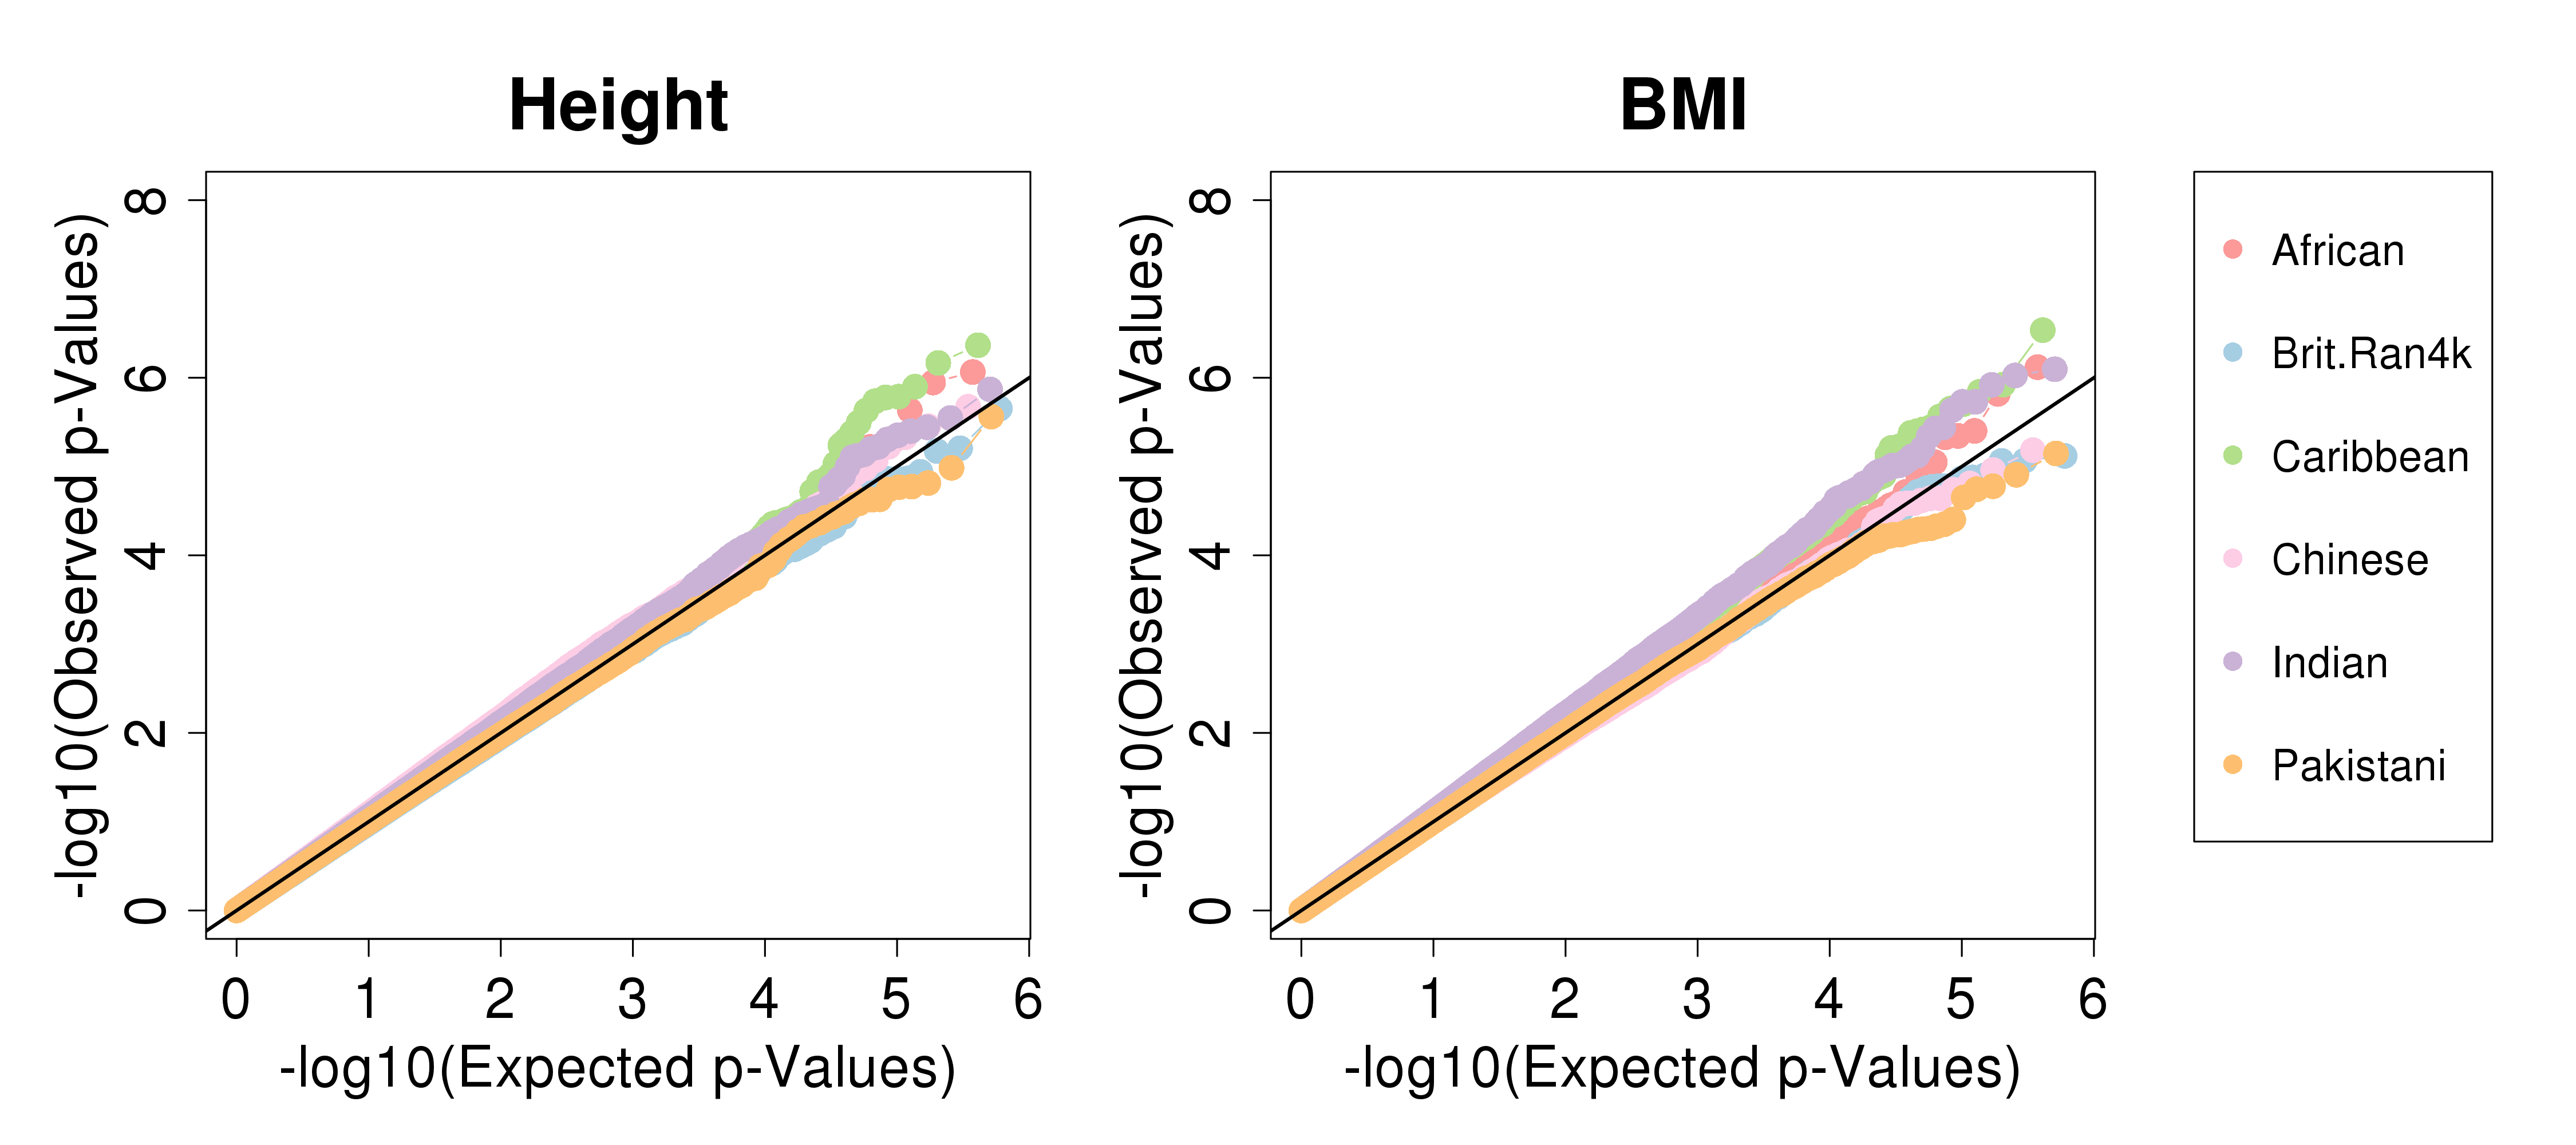
\includegraphics[scale=.45]{Images/Main/InterPath_Main_Figure_MAPIT_vs4_HeightBMI.png}
%\caption[TBD]{\textbf{QQ-Plots of MAPIT results, per subgroup}. The figure shows QQ-plots of our results from running MAPIT on our four initial UKB population subgroups in height and BMI. On the $x$-axis are the -$\log_{10}$ of the expected $p$-values and the on the $y$-axis are on the -$\log_{10}$ of the observed $p$-values. Each data point is a SNP and total SNP counts per UKB subgroup can be found in Supplementary Table \ref{InterPath-Supp-Table-UKBPopStats}. We observe no genome-wide significant signals in any subgroup across both phenotypes ($p$-value $< 5\times10^{-8}$) and, due to this lack of significant results, observe no clear differences in patterns between our subgroups.}
%\label{InterPath-Supp-Figure-MAPIT-HeightBMI}
%\end{figure}

%\begin{figure}[htbp]
%\centering
%\hspace*{-1.7cm}
%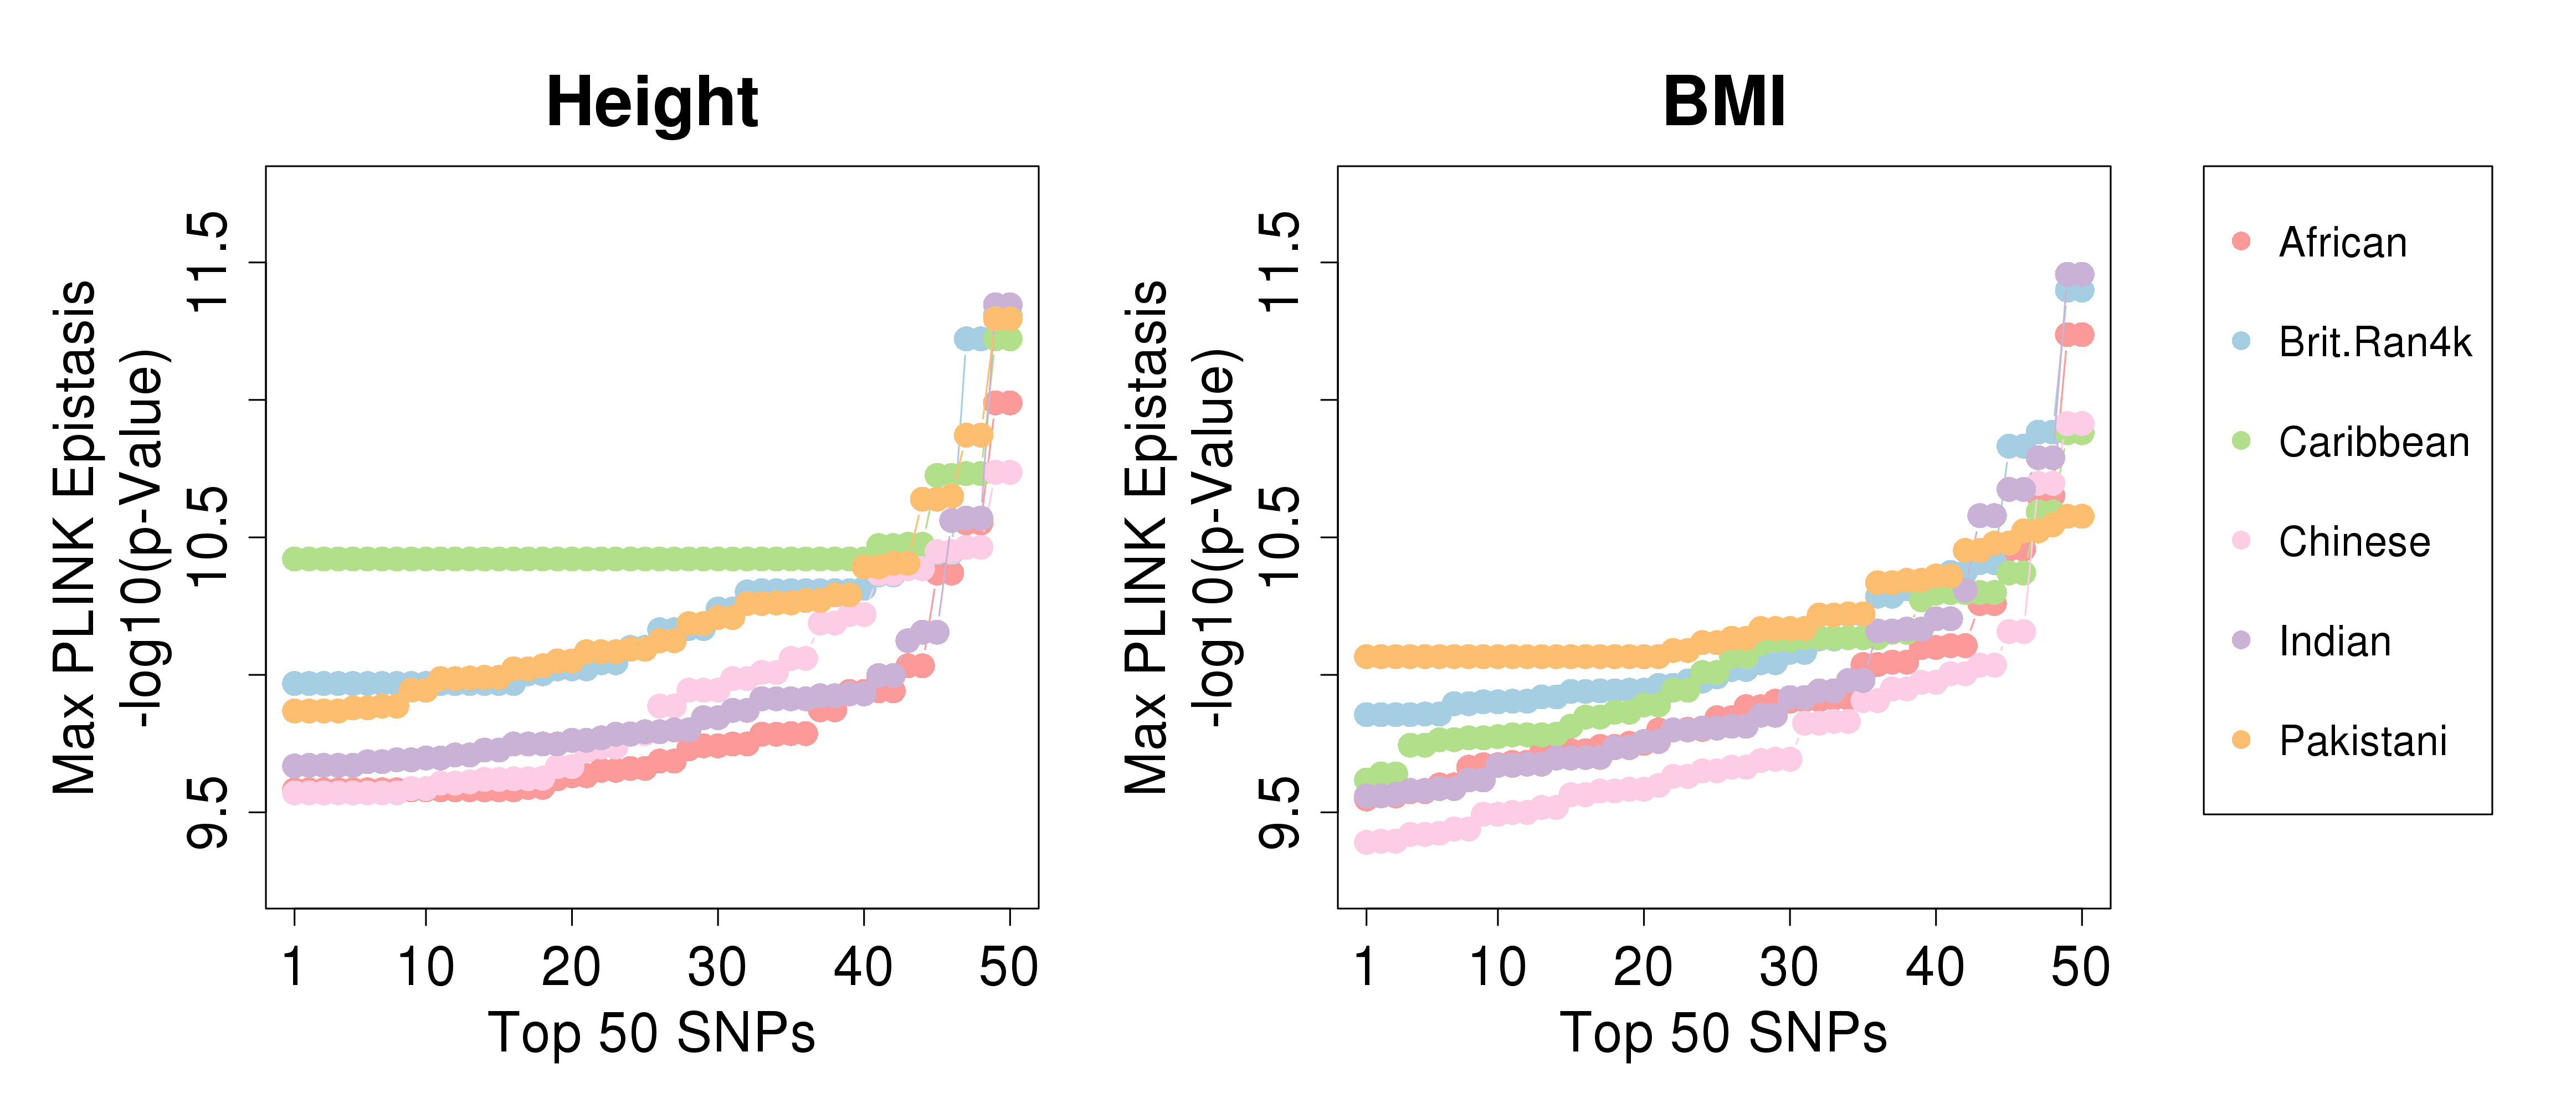
\includegraphics[scale=.45]{Images/Supp/InterPath_Supp_Figure_PLINK_BestSNPs_vs2_AllPops_HeightBMI.png}
%\caption[TBD]{\textbf{SNPs with the largest PLINK pairwise epistasis signals, per subgroup}. The figure shows the best $p$-values obtained from running PLINK's exhaustive pairwise SNP epistasis test for both height and BMI in each of the UKB subgroups. Only the top 50 SNPs, sorted by best pairwise SNP epistasis $p$-value, for each subgroup are shown. No test reaches genome-wide significance based on using a Bonferroni-corrected $p$-value threshold ($p$-value $< 5\times10^{-13}$).}
%\label{InterPath-Supp-Figure-PLINK-HeightBMI-AllPops}
%\end{figure}
%\clearpage





%\addtocounter{figure}{-1}
%\begin{figure} [t!]
%  \caption{\textbf{Number of SNPs in a pathway versus a pathway's MAPIT-R $p$-value}. The figure shows plots comparing the MAPIT-R $p$-values from our main analysis to the number of SNPs present in each pathway. Results for every pathway database-phenotype-UB subgroup combinations are shown. The dotted red line is the line of best fit and the legend provides the regression coefficient and its associated $p$-value. We observe that for most combinations there is a significant relationship between MAPIT-R $p$-value and the number of SNPs present in a pathway. This follows our hypothesis that combining SNPs together in a joint analysis might provide greater power to detect marginal epistasis than analyzing each SNP independently. We note, however, that these results appear to not solely be driven just by the presence or absence of large SNP counts -- conducting this same analysis on one of our sets of permuted phenotypes we now find very few significant relationships between MAPIT-R $p$-values and pathway SNP counts (Supplementary Figure \ref{InterPath-Supp-Figure-pValsVsNumSNPs-perm1}).}
%\label{InterPath-Supp-Figure-pValsVsNumSNPs-Caption}
%\end{figure}
%\clearpage

%\addtocounter{figure}{-1}
%\begin{figure} [t!]
%  \caption{\textbf{Number of SNPs in a pathway versus a pathway's MAPIT-R $p$-value using permuted phenotypes}. The figure shows plots comparing the MAPIT-R $p$-values from our main analysis to the number of SNPs present in each pathway. For this analysis a single set of our permuted phenotypes (i.e. Supplementary Figure \ref{InterPath-Supp-Figure-perm1-QQPlots-AllPaths}) was used for each UKB subgroup. Results for every pathway database-phenotype-subgroup combination is shown. The dotted red line is the line of best fit and the legend provides the regression coefficient and its associated $p$-value. We observe that for very few combinations there is any relationship between MAPIT-R $p$-value and the number of SNPs present in a pathway. For the same analysis on the original set of observed phenotypes, see Supplementary Figure \ref{InterPath-Supp-Figure-pValsVsNumSNPs}.}
%\label{InterPath-Supp-Figure-pValsVsNumSNPs-perm1-Caption}
%\end{figure}
%\clearpage


\setlength{\footskip}{3cm}
\begin{figure}[htbp]
\centering
\vspace*{-2cm}
\includegraphics[scale=.2]{Images/Supp/InterPath_Supp_Figure_IBS_AllPops_vs4_noHLA.png}
\caption[TBD]{\textbf{Pathway-level genetic diversity vs. MAPIT-R results for all database-phenotype-subgroup combinations}. Caption continued on next page.}
\label{InterPath-Supp-Figure-IBS-AllPops}
\end{figure}
\clearpage
\setlength{\footskip}{1cm}
\addtocounter{figure}{-1}

\begin{figure} [t!]
\caption[TBD]{\textbf{Pathway-level genetic diversity vs. MAPIT-R results for all database-phenotype-subgroup combinations}. The figure shows the mean pairwise IBS proportions per pathway plotted against each pathway's MAPIT-R $p$-value for every pathway database-phenotype-UKB subgroup combination. IBS proportions were calculated per pathway by using that pathway's set of SNPs, were calculated pairwise between every set of individuals in the subgroup, and then averaged across each of these pairs for a final, single summary metric. We observe across the majority of combinations no significant relationship between mean pairwise IBS proportion and MAPIT-R $p$-value.}
\label{InterPath-Supp-Figure-IBS-AllPops-Caption}
\end{figure}
\clearpage

%\begin{figure}[htbp]
%\centering
%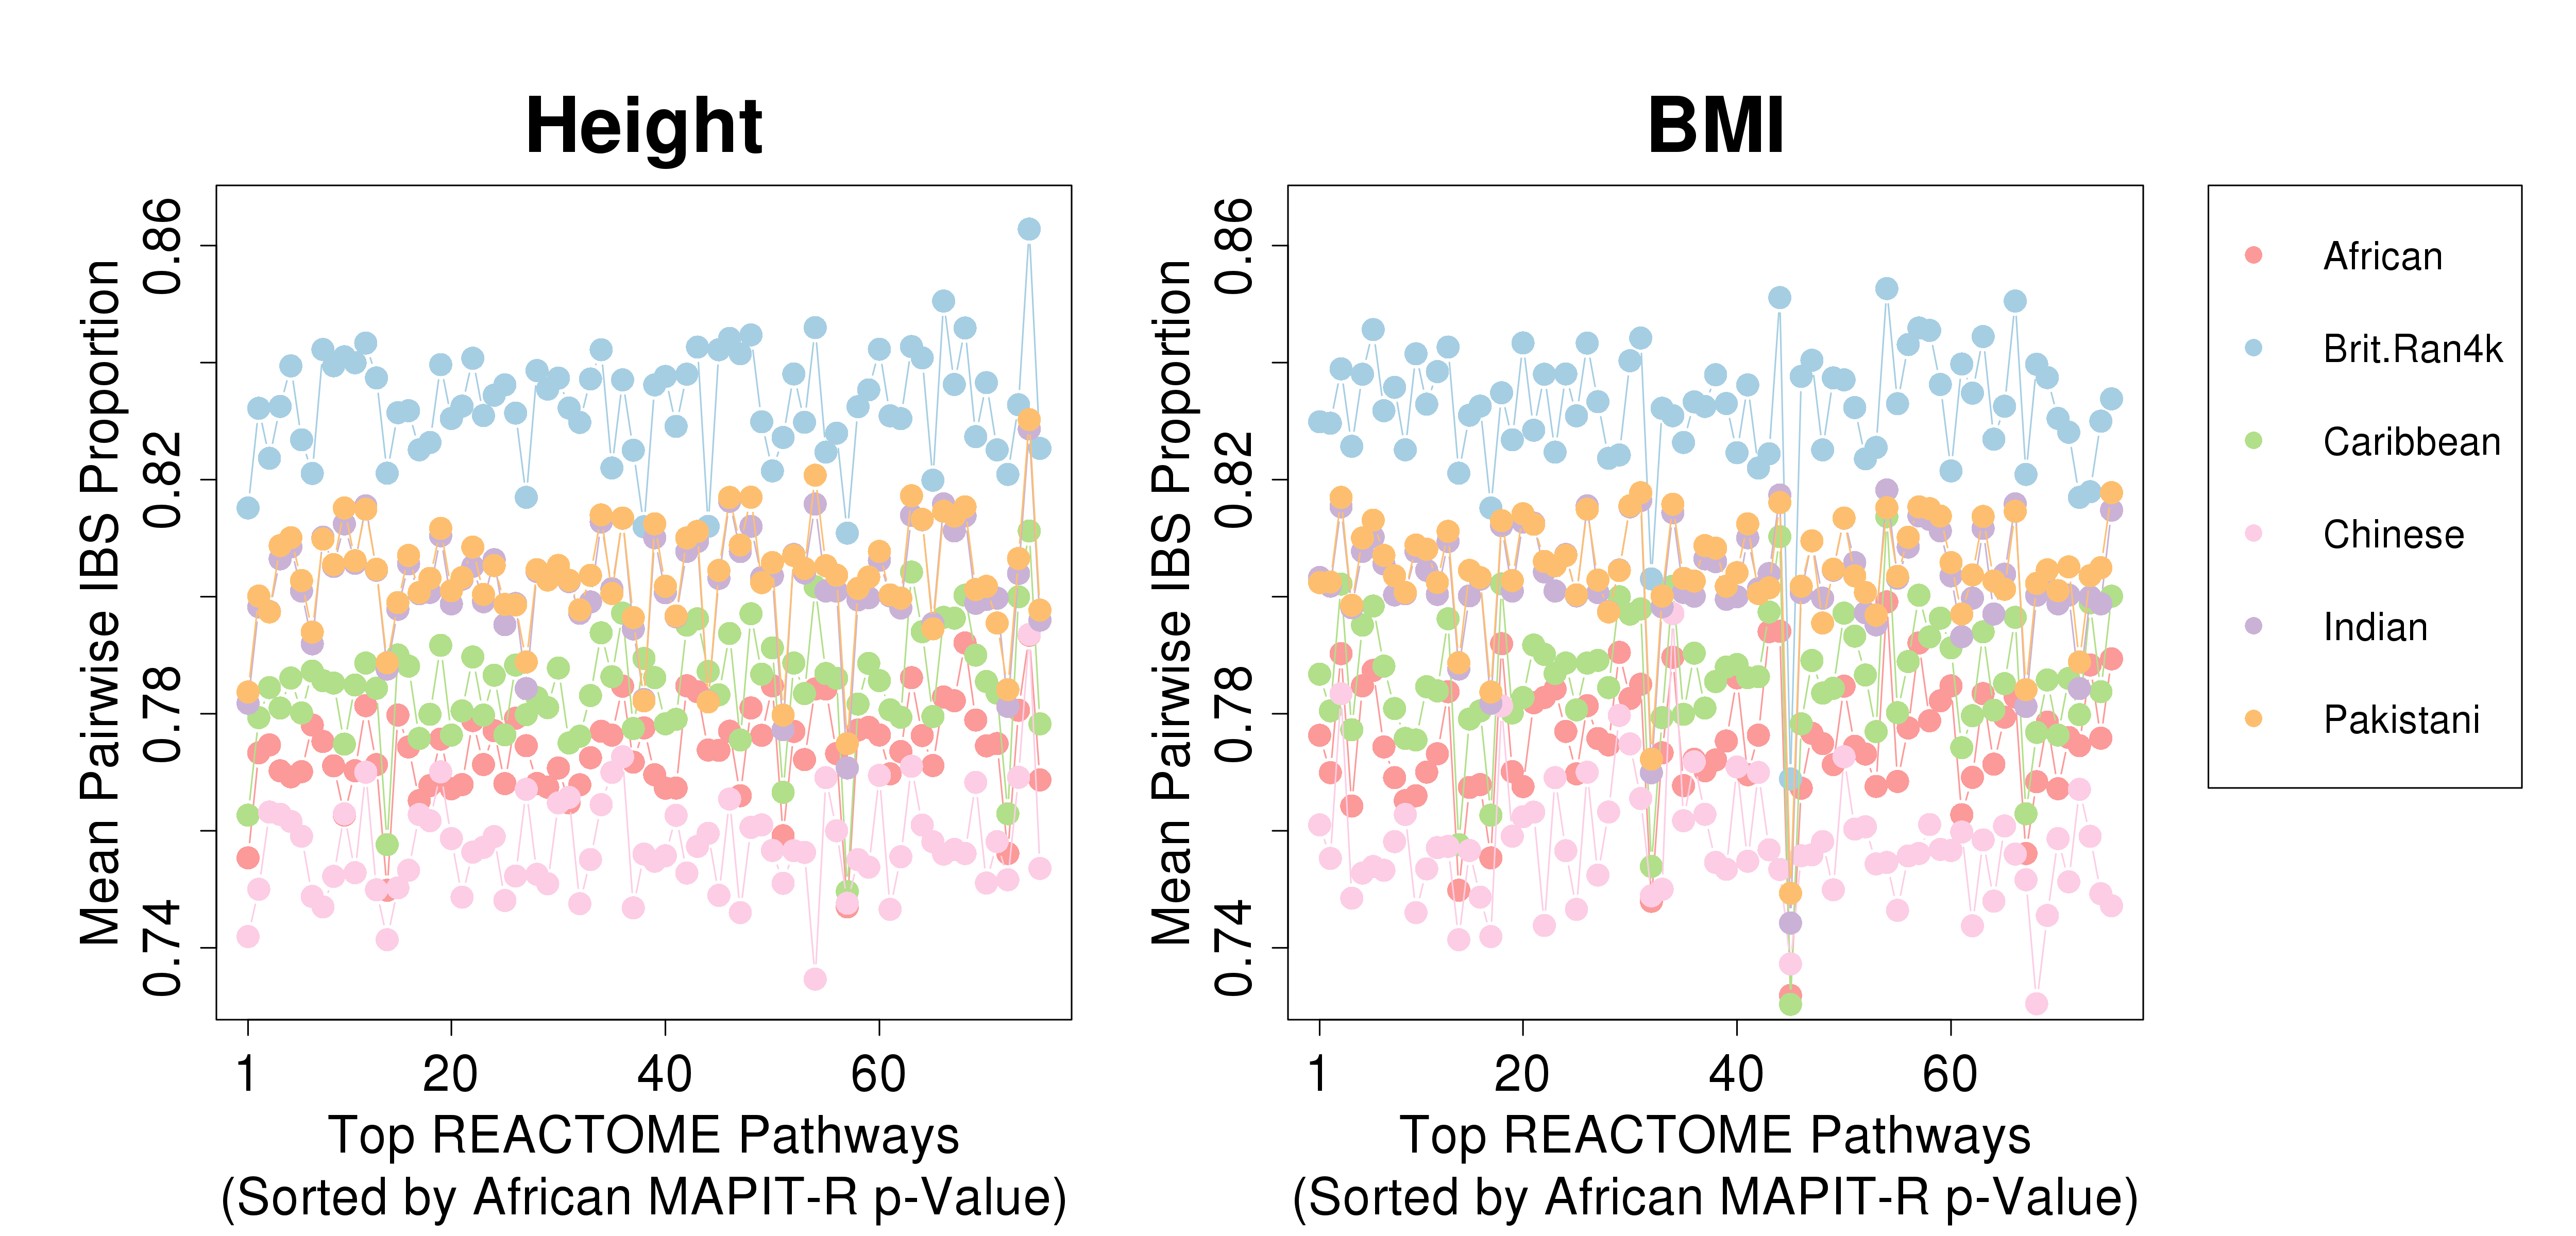
\includegraphics[scale=.35]{Images/Supp/InterPath_Supp_Figure_IBS_AllPopComps_vs3_REACTOME.png}
%\caption[TBD]{\textbf{Pathway-level genetic diversity across all UKB subgroups for top African MAPIT-R REACTOME pathways}. The figure plots the mean pairwise IBS proportions of each UKB subgroup for the top 75 REACTOME pathways (sorted by MAPIT-R African subgroup $p$-value) for each pathway database-phenotype combination. Most variation in mean pairwise IBS proportions varies moreso based on the pathways themselves and not on ancestry; subgroups differ between one another mostly at the same levels across each pathway.}
%\label{InterPath-Supp-Figure-IBS-AllPopComps-REACTOME}
%\end{figure}
%\clearpage

\begin{figure}[htbp]
\centering
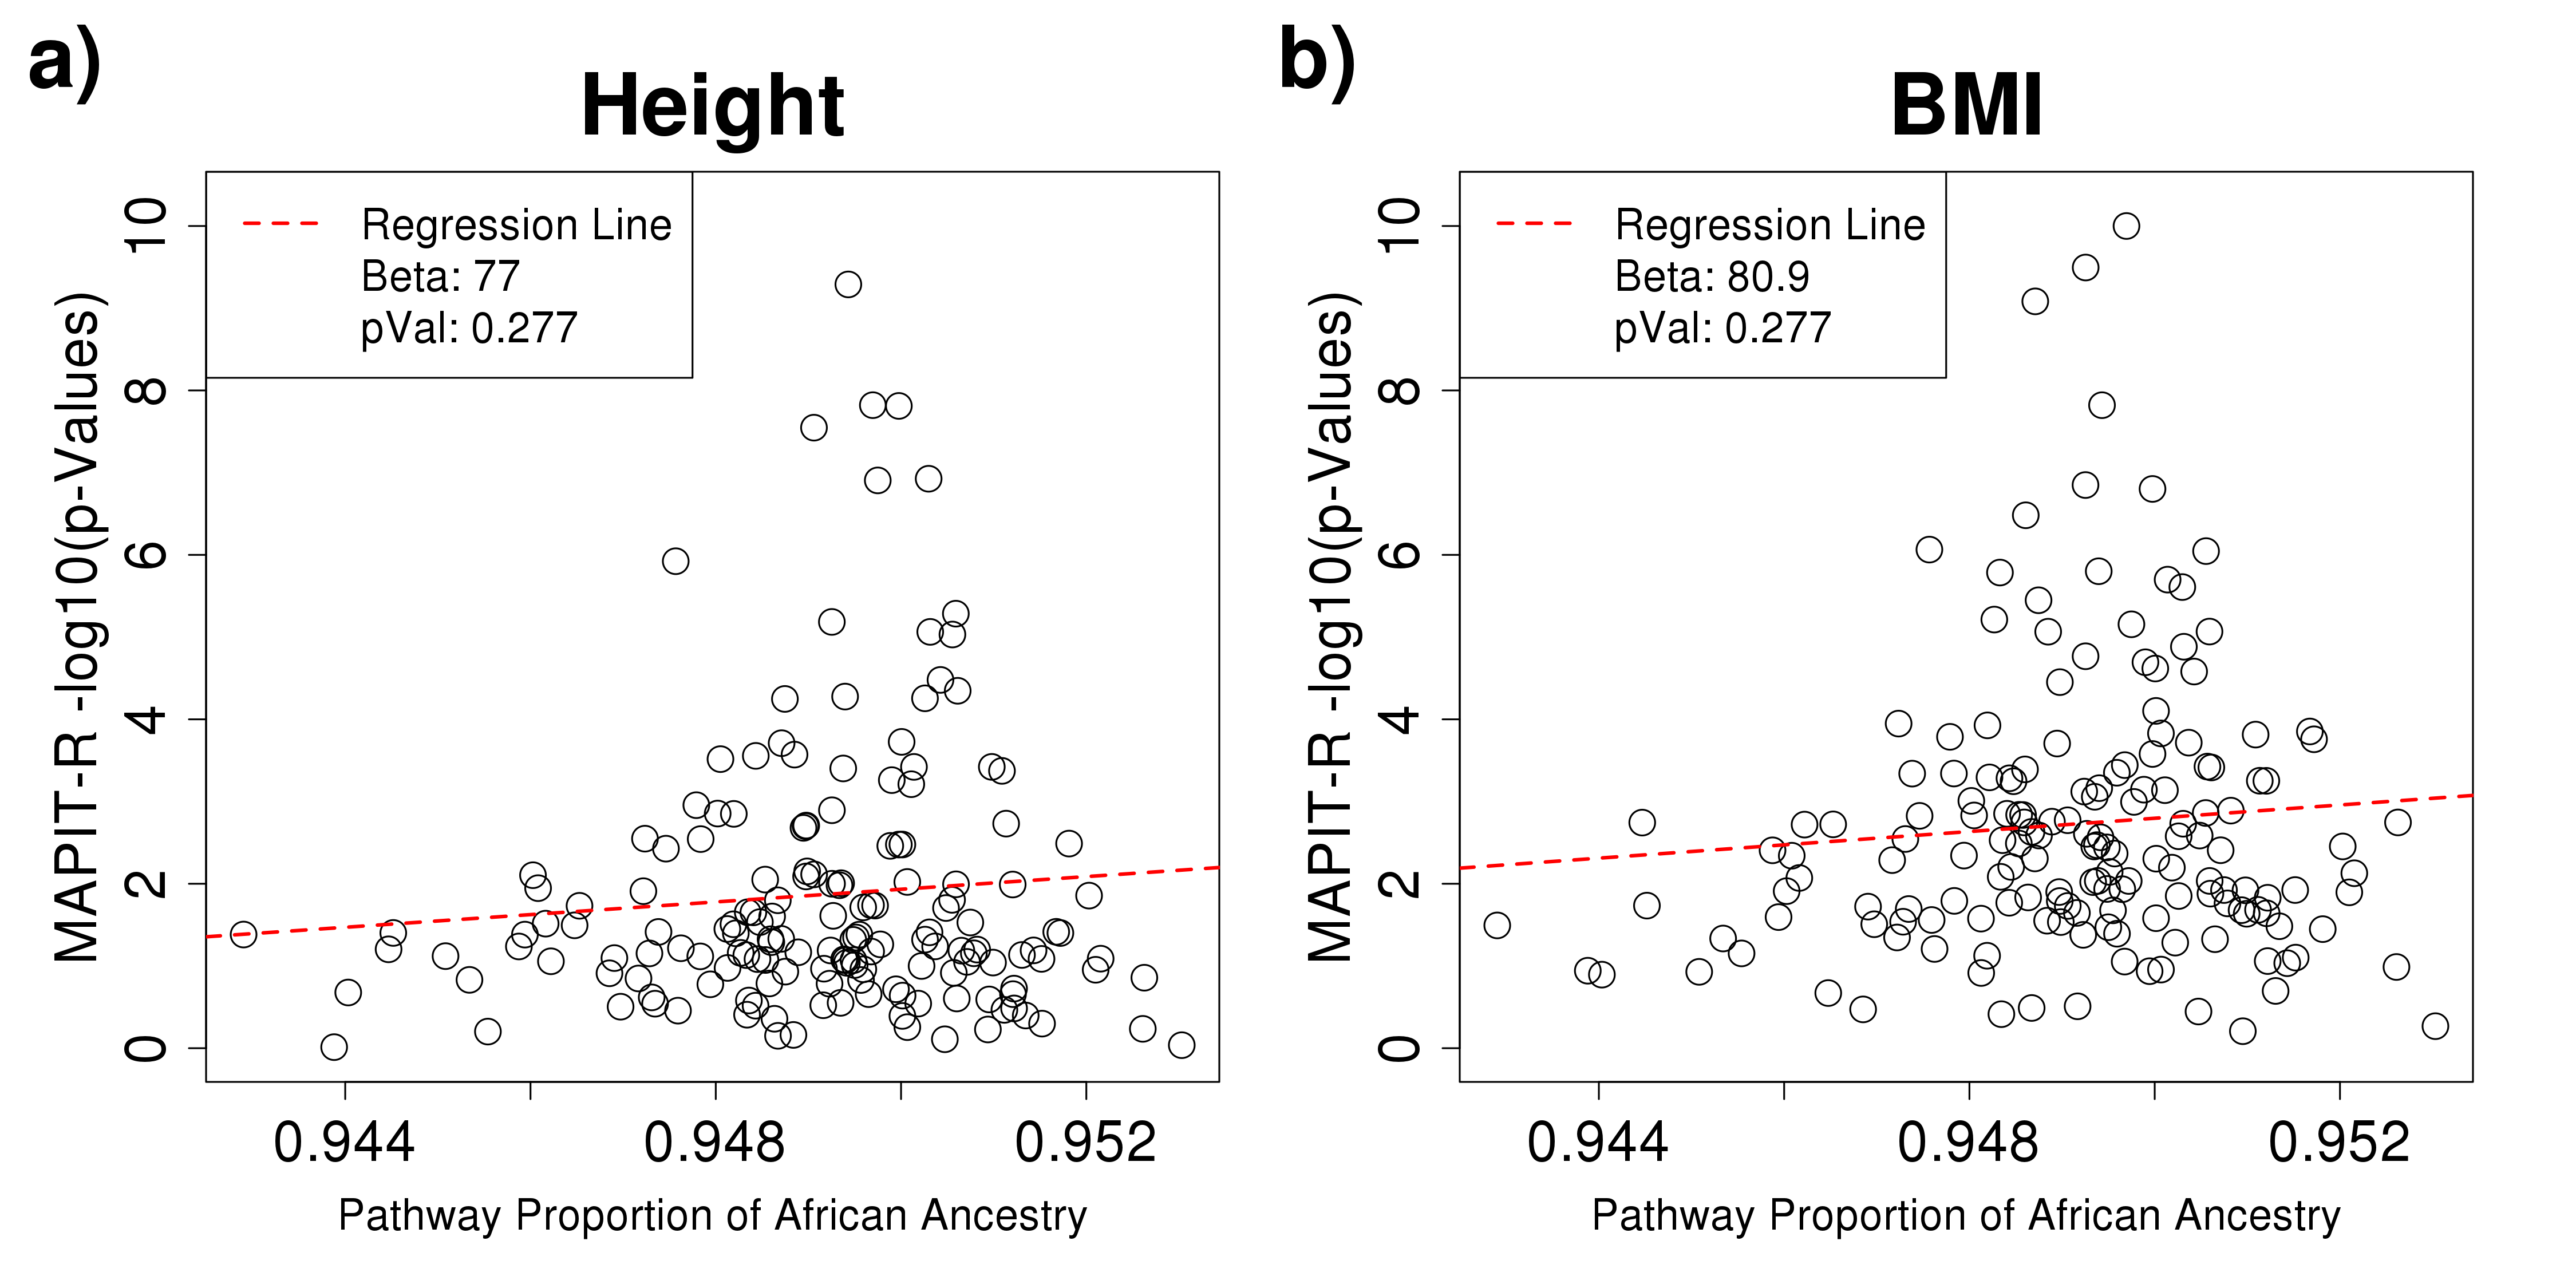
\includegraphics[scale=.35]{Images/Supp/InterPath_Supp_Figure_RFMix_vs2_African_KEGG_noHLA.png}
\caption[TBD]{\textbf{Pathway-level genetic diversity vs. MAPIT-R results in the African subgroup and KEGG database}. The figure shows the mean pairwise IBS proportions per pathway plotted against each pathway's MAPIT-R $p$-value for the African subgroup KEGG (a) height and (b) BMI analysis. IBS proportions were calculated per pathway by using each pathway's set of SNPs to derive pairwise IBS values between every set of individuals in the subgroup, and then averaging across each of these pairs for a final summary metric. Results with REACTOME database pathways can be found in Supplementary Figure \ref{InterPath-Main-Figure-RFMix-African-REACTOME}. We observe across the majority of our combinations no significant relationship between a pathway's mean pairwise IBS proportion and its MAPIT-R $p$-value.}
\label{InterPath-Supp-Figure-RFMix-African-KEGG}
\end{figure}
\clearpage

\setlength{\footskip}{3cm}
\begin{figure}[htbp]
\centering
\vspace*{-2cm}
\includegraphics[scale=.2]{Images/Supp/InterPath_Supp_Figure_PC1Loading_AllPaths_vs2_noHLA.png}
\caption[TBD]{\textbf{Relationship between MAPIT-R $p$-values and proportions of pathway SNPs loaded on PC1, all pathways}. Caption continued on next page.}
\label{InterPath-Supp-Figure-PC1Loading-AllPaths}
\end{figure}
\clearpage
\setlength{\footskip}{1cm}

\addtocounter{figure}{-1}
\begin{figure} [t!]
  \caption{\textbf{Relationship between MAPIT-R $p$-values and proportions of pathway SNPs loaded on PC1, all pathways}. The figure shows the proportion of SNPs within a given pathway that are strongly loaded on local PC1 plotted against that pathway's MAPIT-R -$\log_{10}$ $p$-value. All pathway sizes were used for this analysis. `Local' here refers to PCA having been conducted within-subgroup. SNPs are designated as `strongly loaded' on local PC1 if they are within the 10\% tails of the loading SNP score distributions. We observe that there is no significantly positive relationship between MAPIT-R $p$-values and proportion of SNPs that are strongly loaded on PC1 for any pathway database-phenotype-subgroup combination.}
\label{InterPath-Supp-Figure-PC1Loading-AllPaths-Caption}
\end{figure}
\clearpage


%Ten pathways were constructed by selecting 50 random SNPs for each pathway and another 200 SNPs were randomly selected to be `interacting partners' for each pathway SNP. Additionally, 50\% of the remaining SNPs were selected to represent the additive background. Next, we simulate continuous phenotypes by using the following model: $\by = \bZ\bu + \bX\bbeta + \bW\ba + \bepsilon$, where $\bX$ is the genotype matrix, $\bZ$ contains covariates representing population structure, and $\bu$ are fixed effects. Under this model we simulate additive effect sizes for each SNP in the additive background and the random noise term from a standard normal distribution, and then we scale the two terms to further ensure a narrow-sense heritability of either 60\% or 80\%. We also introduce 
%Phenotypes were constructed by simulating both additive and epistatic components. Epistatic components were constructed by simulating interactions between pathways and the rest of the genomic background. Specifically, 10 pathways were used in each simulation, where each pathway contained 50 SNPs. For each pathway, every SNP was considered an `interacting' SNP, meaning each SNP had 200 `interacting partner' SNPs randomly chosen elsewhere from among the remaining 9,950 background SNPs. To simulate the additive heritability component, an additional 50\% of the background, non-interacting SNPs were assigned additive effects. Overall heritability ($H^2$) was set at .6 or .8. Additive heritability was set at $H^2*(\rho)$ and epistatic heritability was set at $H^2*(1-\rho)$, where $\rho$ is a value ranging from .6 to .9 that controls the ratio between additive and epistatic heritability. Lastly, the top 10 local principal components of the individuals were used to introduce population structure and account for 10\% of the overall phenotype variance. (a) The barplots show power and false discovery rates (FDR) from running the aforementioned MAPIT-R simulations. $H^2$ of .6 is shown on the left and $H^2$ is shown on the right. The $x$-axis shows the different values of $\rho$ and the $y$-axis shows power. Colors correspond to different value of $\rho$ and the legend shows each corresponding FPR.
%Phenotypes were constructed by simulating both additive and epistatic components. Epistatic components were constructed by simulating interactions between pathways and the rest of the genomic background. Specifically, 10 pathways were used in each simulation, where each pathway contained 50 SNPs. For each pathway, every SNP was considered an `interacting' SNP, meaning each SNP had 200 `interacting partner' SNPs randomly chosen elsewhere from among the remaining 9,950 background SNPs. To simulate the additive heritability component, an additional 50\% of the background, non-interacting SNPs were assigned additive effects. Overall heritability ($H^2$) was set at .6 or .8. Additive heritability was set at $H^2*(\rho)$ and epistatic heritability was set at $H^2*(1-\rho)$, where $\rho$ is a value ranging from .6 to .9 that controls the ratio between additive and epistatic heritability. Lastly, the top 10 local principal components of the individuals were used to introduce population structure and account for an additional 10\% of the overall phenotype variance.
%To simulate continuous phenotypes that mirror genetic architectures affected by a combination of additive and pairwise epistatic effects, we randomly choose 1,000 causal SNPs to directly affect the phenotype and classify the causal variants into three groups: (1) a small set of interaction SNPs, (2) a larger set of interaction SNPs, and (3) a large set of additive SNPs. In the simulations carried out in this study, SNPs interact between sets, so that SNPs in the first group interact with SNPs in the second group, but do not interact with variants in their own group (the same rule applies to the second group). One may view the SNPs in the first set as the “hubs” in an interaction map. We are reminded that interaction (epistatic) effects are different from additive effects. All causal SNPs in both the first and second groups have additive effects and are involved in pairwise interactions, while causal SNPs in the third set only have additive effects.
%The additive effect sizes of all causal SNPs again come from a standard normal distribution or β ∼ MVN(0, I). Next, we create a separate matrix W which holds the pairwise interactions of all the causal SNPs between groups 1 and 2. These SNPs have effect sizes also drawn as α ∼ MVN(0, I). We scale both the additive and pairwise genetic effects so that collectively they explain a fixed proportion of genetic variance. Namely, the additive effects make up ρ\%, while the pairwise interactions make up the remaining (1 − ρ)%. Once we obtain the final effect sizes for all causal SNPs, we draw errors to achieve the target H2. The phenotypes are then created by summing all effects using two simulation models: (i) y = Xβ + Wα + ε and (ii) y = Zu + Xβ + Wα + ε, where Zu again represents population stratification. In the latter model, population stratification effects are introduced into the simulations by allowing the top 5 and 10 genotype principal components (PCs) Z to make up 10% of the overall variation in the trait. The effect sizes for these stratification effects are also drawn as u ∼ MVN(0, I)
%Each pathway has